\documentclass[12pt,a4paper]{article}

\usepackage[T2A]{fontenc}
\usepackage[utf8]{inputenc}
\usepackage[russian,english]{babel}
\usepackage[a4paper, margin=2.2cm]{geometry}
\usepackage{amsmath,amssymb,amsthm}
\usepackage{graphicx}
\usepackage{booktabs}
\usepackage{array}
\usepackage{longtable}
\usepackage{enumitem}
\usepackage{xcolor}
\usepackage{hyperref}
\usepackage{placeins}
\usepackage{float}
\hypersetup{
  colorlinks=true,
  linkcolor=black,
  urlcolor=blue,
  citecolor=blue,
}
\renewcommand{\arraystretch}{1.15}
\setlength{\parindent}{1.25em}
\setlength{\parskip}{0.4ex}
\sloppy

\title{Применимость процессов Хокса для предсказания пользовательской активности в e-commerce}
\author{Алексей Мошкин\\\small МКН СПбГУ\\\small Научный руководитель: Николаев Максим Сергеевич}
\date{2026}

\begin{document}

\maketitle

\section*{Аннотация}
\addcontentsline{toc}{section}{Аннотация}

Работа посвящена применению процессов Хокса для предсказания дневной интенсивности покупок пользователя в e-commerce. Прогноз пользовательской активности - важный блок при оценке ценности клиента, планировании коммуникаций с ним и подведении итогов A/B-экспериментов. Точные модели интенсивности позволяют не только улучшать бизнес-метрики, но и интерпретировать структуру пользовательского поведения. А процессы Хокса с экспоненциальным ядром естественно описывают самовозбуждение и кросс-канальные влияние событий и при этом сохраняют легко интерпретируемые параметры, что выгодно отличает их от более сложных моделей машинного обучения, например бустингов.

Актуальность работы обусловлена тем, что в индустриальных задачах с разреженными счётчиками (доля нулей в нашем датасете - \texttt{93.7\%}) большинство стандартных регрессионных методов теряет в качестве из-за дисбаланса, тогда как явная вероятностная модель с Хоуск ядрами остаётся стабильной и легко интерпретируется. В работе исследуется не только предсказательное качество Хоукс-моделей, но и их сходимость, чувствительность к выбору регуляризации, идентифицируемость коэффициентов и поведение на разных длинах обучающего окна - то есть аспекты, важные для практического применения модели.

В качестве данных используется датасет из \texttt{10K} пользователей крупного маркетплейса за \texttt{290} дней с пятью поведенческими счётчиками (\texttt{searches}, \texttt{cat\_to\_cart}, \texttt{cat\_to\_ord}, \texttt{to\_cart}, \texttt{to\_ord}). Основной target - число покупок \texttt{to\_ord} на пару \texttt{(user, day)}. Все эксперименты проводятся на воспроизводимом коде на Python.

Основные результаты: построена иерархия из шести вероятностных моделей с переходом от Global Poisson к Joint Hawkes; на главном \texttt{207}-дневном train-test разбиение Хоукс-надстройка устойчиво улучшает персонализированный пуассоновский бейзлайн на трёх независимых каналах; кросс-канальная матрица $\alpha  \in  \mathbb{R}^{3\times 3}$ восстановлена в виде нижнетреугольной структуры воронки \texttt{searches → to\_cart → to\_ord}. Через ландшавт лосса показано, что диагональные коэффициенты слабо идентифицируемы, что согласуется с известными результатами по многоядерным Хоукс процессам [4, 5]; бустинг на богатых данных после feature-engineering(построена 141 фича) даёт верхнюю планку качества, но с менее интерпретируемой структурой. Дополнительно проведёно исследование, показывающие, что эффект от Хоукс ядер сильно скоррелирован с настройками базовой интенсивности, за счет этого возможен "переток массы" между Хоукс-частью и базовой интенсивностью без значительной потери качество, из-за чего выбор регуляризации(численной или структурной) очень важен, так как именно он регулирует где остенется масса. Особенно сильно этот эффект проявляется на коротких train-test окнах, где в зависимости от регуляризации веса Хоукс ядер могут полностью обнулиться. 

\tableofcontents
\clearpage
\section{Введение}

\FloatBarrier
\subsection{Постановка задачи и актуальность}

Задача предсказания пользовательской активности - одна из центральных в современном e-commerce. Точная оценка ожидаемого числа покупок \texttt{to\_ord} на пару \texttt{(user, day)} может напрямую использоваться в персонализации ранжирования, расчёте CLV и подведении итогов A/B-экспериментов. 

С формальной точки зрения мы оцениваем дневную интенсивность $\lambda _{u,t}$ и предполагаем условную Пуассоновскую модель наблюдения:

\[
y_{u,t} \mid \lambda_{u,t} \;\sim\; \mathrm{Poisson}(\lambda_{u,t}),
\]

где \texttt{y\_\{u,t\}} - число покупок пользователя \texttt{u} в день \texttt{t}, а $\lambda _{u,t}$ - наша точечная оценка интенсивности. Задача состоит в предсказании $\lambda _{u,t}$ на отложенную тестовой выборке. 

Особенность задачи - крайняя разреженность сигнала: в наших данных среднее число покупок на \texttt{(user, day)} $\approx$ \texttt{0.10}, а доля нулевых ячеек - \texttt{93.7\%}. Такие данные плохо подходят к классическим регрессионным методам, ориентированным на нормальные ошибки, и требуют явного учёта Пуассоновского распределения наблюдений. Дополнительная сложность - сильное различие в поведение пользователей: разброс по среднему числу покупок между пользователями на порядки превышает изменчивость во времени, поэтому без персонализации модель работает плохо.

Третья особенность - событийный характер сигнала. Покупки не происходят равномерно во времени: часто наблюдаются «вспышки» активности (пользователь сделал серию заказов за один-два дня) с последующей длительной паузой. Для моделирования такой динамики могут применяться self-exciting процессы, в котором недавние события явно влияет на интенсивность будущих событий, и.

Актуальность работы определяется тремя факторами. Во-первых, индустриальные системы прогноза покупок чаще всего опираются на слабо интерпретируемые модели (GBDT, нейросети), которые дают хороший скор, но не дают понимания структуры пользовательского поведения. Во-вторых, при оценке эффектов A/B-экспериментов важно не только качество прогноза, но и стабильность модели на коротких окнах и интерпретируемость её параметров - здесь GBDT с сотнями признаков становится плохо контролируемым инструментом. В-третьих, процессы Хокса, успешно применявшиеся в финансах [2] и анализе кликовых потоков [3, 7], редко рассматриваются в индустриальном e-commerce как полноценный инструмент - несмотря на то, что их параметры (per-user multiplier, матрица $\alpha$-взаимодействий) допускают прямую бизнес-интерпретацию.

\FloatBarrier
\subsection{Процессы Хокса: специфика и применимость к задаче}

Процесс Хокса - это самовозбуждающийся точечный процесс, в котором интенсивность будущих событий зависит от истории уже случившихся [1]. В классической непрерывной форме одномерный процесс с экспоненциальным ядром записывается как

\[
\lambda(t) \;=\; \mu \;+\; \sum_{t_i < t} \alpha \cdot \exp\!\left(-\beta (t - t_i)\right),
\]

где $\mu $ - фоновая интенсивность, $\alpha $ - вес возбуждения, а $\beta $ - скорость затухания сигнала. 
Каждое произошедшее событие повышает интенсивность в ближайшем будущем. Свойство "памяти" этого процесса - конечное: после нескольких полураспадов событие фактически перестаёт влиять на текущую интенсивность.

В многомерной форме (\texttt{K} типов событий) ядра становятся матричными:

\[
\lambda_k(t) \;=\; \mu_k \;+\; \sum_{j=1}^{K} \sum_{t_i^{(j)} < t} \alpha_{kj} \cdot \exp\!\left(-\beta_{kj} (t - t_i^{(j)})\right).
\]

Здесь $\alpha _{kj}$ интерпретируется как «сила влияния события типа \texttt{j} на интенсивность типа \texttt{k}». Эта матричная структура и есть та самая cross-channel матрица, которая в нашей работе восстанавливается для воронки \texttt{searches → to\_cart → to\_ord}.

В дискретно-дневной форме, удобной для нашей задачи, мы пишем

\[
\lambda_{u,t} \;=\; \underbrace{\mu_{u,t}}_{\text{baseline}} \;+\; \sum_{j} \alpha_j \cdot z_{u,j,t},
\]

где $\mu _{u,t}$ - уверенный бейзлайн пользовательской интенсивности, построим его чуть позже, а \texttt{z\_\{u,j,t\}} - экспоненциально сглаженный счётчик \texttt{j}-ой фичи у пользователя \texttt{u} до дня \texttt{t}:

\[
z_{u,j,t} \;=\; \sum_{s < t} x_{u,j,s} \cdot \exp\!\left(-\frac{t - s}{\tau_j}\right),
\]

с заданным полураспадом $\tau _j$ (в большинстве экспериментов мы используем $\tau  \in  \{1, 3\}$ дня). Веса $\alpha _j$ оцениваются по обучающей выборке и допускают прямую интерпретацию: положительный $\alpha _j$ означает, что событие фичи \texttt{j} повышает интенсивность будущих покупок этого пользователя.

Применимость процессов Хокса к нашей задаче объясняется следующими свойствами:

\begin{enumerate}
  \item \textbf{Self-excitation естественно описывает воронку покупок.} В e-commerce покупка не происходит «из ниоткуда»: ей часто предшествует серия поисков, просмотров и добавлений в корзину. Hawkes явно моделирует эту короткую память.
  \item \textbf{Параметры интерпретируемы.} Матрица $\alpha [target \leftarrow  source]$ показывает, какие каналы и в какой мере возбуждают другие каналы. Это даёт бизнес-понимание, недоступное у GBDT.
  \item \textbf{Аддитивная декомпозиция бейзлайн + надстройка.} Модель явно разделяет «фоновую активность» пользователя и «короткие всплески от событий», что позволяет независимо изучать обе компоненты.
\end{enumerate}


Платой за интерпретируемость становится более ограниченная функциональная форма: линейная additive комбинация $\lambda _u \cdot  b\_t + \alpha ^{\top} z$ игнорирует нелинейные взаимодействия признаков, которые GBDT мог бы учесть. Оценка того, насколько много полезной информации при таком упращении мы теряем - одна из задач работы.

\FloatBarrier
\subsection{Цели и задачи работы}

\textbf{Цель работы}: исследовать границы применимости процессов Хокса для предсказания дневной интенсивности покупок пользователя в e-commerce, оценить их предсказательное качество и стабильность по сравнению с вероятностным бейзлайном и бустинговой моделью, а также изучить идентифицируемость и интерпретируемость их коэффициентов.

\textbf{Задачи работы}:

\begin{enumerate}
  \item Построить иерархию вероятностных моделей, дающую устойчивый бейзлайн для последующей Хоукс-надстройки.
  \item Исследовать особенности сходимости коэффициентов Хоукс-моделей: на каком объёме train они стабилизируются и какая параметризация подходит для коротких окон.
  \item Восстановить cross-channel матрицу $\alpha [target \leftarrow  source]$ для трёх каналов воронки и оценить её устойчивость к выбору train-окна и регуляризации.
  \item Сравнить Хоукс-модель с двумя контрольными моделями - статистическим бейзлайном и бустингом на расширенном feature-engineering'е датасете - на нескольких train-test разбиениях.
\end{enumerate}


\FloatBarrier
\subsection{Используемые данные}

Все эксперименты проводятся на открытом датасете, обезличенно отражающем поведение \texttt{10000} случайно выбранных пользователей крупного e-commerce-сервиса за период \texttt{2025-01-15..2025-10-31} (\texttt{290} дней). На каждую пару \texttt{(user, day)} доступны пять поведенческих счётчиков (число событий за день):

\begin{itemize}
  \item \texttt{searches} - пользовательские поиски, mean $\approx  1.20$ событий на строку;
  \item \texttt{cat\_to\_cart} - переходы из категории в корзину;
  \item \texttt{cat\_to\_ord} - переходы из категории к оформлению заказа;
  \item \texttt{to\_cart} - добавления товаров в корзину, mean $\approx  0.37$;
  \item \texttt{to\_ord} - оформленные заказы (target), mean $\approx  0.10$.
\end{itemize}


Структура данных - длинный pandas DataFrame с \texttt{\textasciitilde{}2.87M} строк формы \texttt{(user\_id, event\_date, searches, to\_cart, to\_ord, ...)}. Все ячейки заполнены явно: даже если пользователь в какой-то день не проявлял активности, в датасете присутствует строка с нулями. Это упрощает построение rolling-агрегатов и Hawkes-states одной свёрткой по каждому пользователю.

\clearpage
\section{Обзор литературы}

Процессы Хокса как класс самовозбуждающихся точечных процессов введены Хоксом [1] и долгое время применялись преимущественно в сейсмологии и финансах [2]. С развитием современных систем сбора пользовательских данных интерес к ним смещается в сторону анализа кликовых потоков, рекомендательных систем и e-commerce.

Существенная часть современной литературы посвящена нейронным расширениям Хоукс-моделей. Du et al. [3] предложили recurrent marked temporal point processes (RMTPP), в которых дискретная история событий пользователя сжимается рекуррентной сетью в вектор состояния, по которому затем предсказывается интенсивность будущих событий. Mei и Eisner [7] развили эту идею в neural Hawkes process, явно параметризовав интенсивность нейросетью, сохраняющей формальную структуру self-exciting процесса. Эти подходы дают высокое качество, но за счёт интерпретируемости: нейросетевой блок становится чёрным ящиком, и непосредственно «прочитать» матрицу cross-channel влияний из обученной модели нельзя.

Параллельно развиваются классические multivariate Хоукс-модели с акцентом именно на интерпретируемость и идентифицируемость. Bacry, Bompaire, Gaïffas и Muzy [4] показывают, что при оценке коэффициентов многомерного Хоукс-процесса по максимальному правдоподобию имеет смысл регуляризовать диагональные элементы матрицы влияния отдельно от внедиагональных: первые отвечают за «свой» self-excitation канала и часто коллинеарны фоновой интенсивности $\mu $, вторые описывают cross-channel взаимодействия и идентифицируются устойчивее. В нашей работе мы наблюдаем эту же асимметрию эмпирически (см. часть III) и связываем её с тем же механизмом коллинеарности history-state и baseline. Параллельно Achab et al. [5] предложили отказ от MLE в пользу integrated cumulants, чтобы обойти проблему non-identifiability диагональных коэффициентов на коротких выборках; их подход не требует точной формы ядер и масштабируется к большим \texttt{K} через спектральные разложения матриц моментов.

В индустриальном контексте предсказания пользовательской активности классическим инструментом остаются модели семейства Pareto/NBD и Beta-Geometric, восходящие к работам Fader и Hardie [6]. Их центральная идея - Gamma-prior на индивидуальный темп покупок пользователя $\lambda _u$, с регуляризацией оценки через Empirical-Bayes posterior. Этот же приём используется нами в Personalized Gamma-Poisson бейзлайне и оказывается основным шагом, дающим крупнейший выигрыш по NLL: при $(\alpha , \beta ) \approx  (0.88, 0.88)$ модель аккуратно ранжирует пользователей по их «истинному» темпу и обеспечивает устойчивую базу для последующей Хоукс-надстройки.

Наконец, для сравнения с интерпретируемой моделью используются современные бустинговые методы, в первую очередь Gradient Boosting Machines в реализации Friedman [8] и их продвинутые версии (\texttt{HistGradientBoosting}, \texttt{LightGBM}, \texttt{CatBoost}). На широком feature-engineering'е такие модели дают верхнюю планку по качеству, особенно когда сигнал содержит нелинейные взаимодействия признаков, плохо схватываемые линейной additive формой Hawkes. Однако они не дают структурных коэффициентов, сопоставимых с матрицей $\alpha $ Хоукс-процесса, и поэтому используются в работе как control, а не как самостоятельная цель.

\clearpage
\section{Разведочный анализ данных и метрика качества}

\FloatBarrier
\subsection{Структура датасета и разреженность}

Панель данных представляет собой плотную таблицу \texttt{(user × day)} без пропусков: для каждого из \texttt{10K} пользователей доступны строки на все \texttt{290} дней анализируемого периода (нулевые счётчики записаны явно). 

Распределение таргета \texttt{to\_ord} крайне разреженное. Гистограмма числа покупок на user-day (log-Y) показана на рис. 1.


\begin{figure}[ht]
\centering
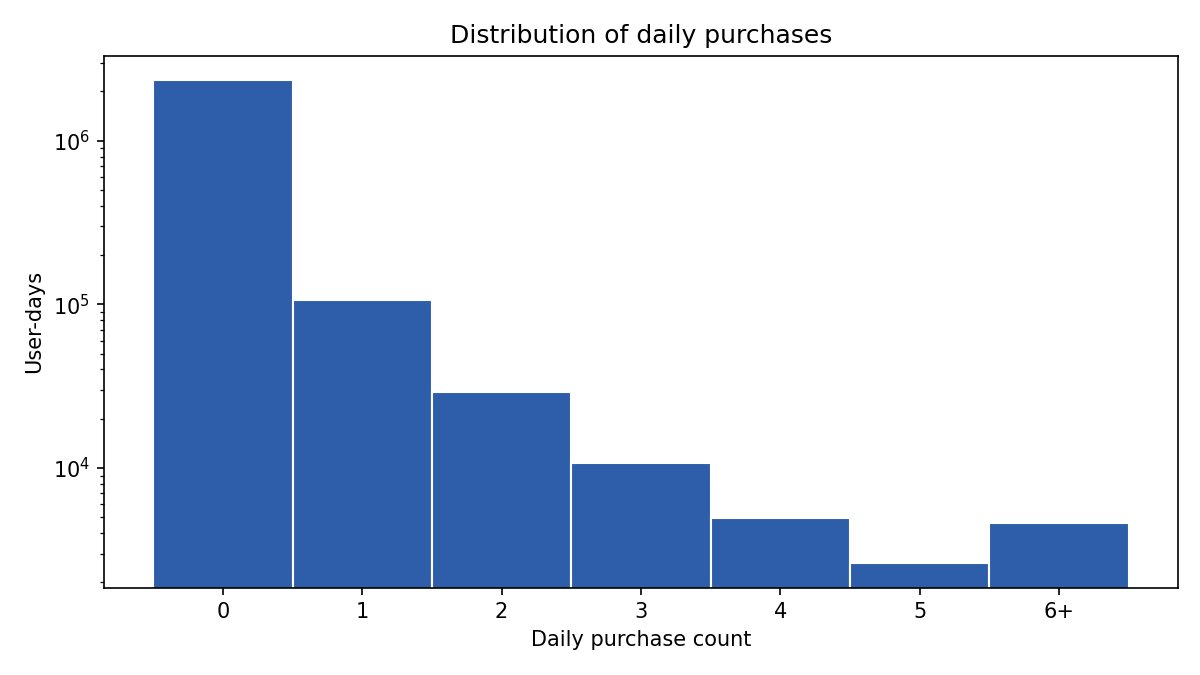
\includegraphics[width=0.85\textwidth]{images/fig01_orders_histogram_logy.jpg}
\caption{Распределение числа покупок на user-day (log-Y)}
\end{figure}


Видны три структурных факта:

\begin{itemize}
  \item Подавляющее большинство ячеек содержат нули - точнее, \texttt{93.7\%} строк датасета имеют \texttt{to\_ord = 0}.
  \item Существует тяжёлый правый хвост: единичные \texttt{(user, day)}-пары содержат десяток покупок и больше, при максимуме порядка сотни. Это означает, что распределение \texttt{to\_ord} имеет крайне тяжелые хвосты.
  \item При этом среднее по данным $\approx  0.10$ - и есть та самая разреженность сигнала.
\end{itemize}


Эта картина мотивирует две вещи. Во-первых, использовать именно Пуассоновскую модель наблюдения, а не нормальную регрессию - иначе при \texttt{93.7\%} нулей оптимум прогноза вырождается в константу около нуля. Во-вторых, явно учитывать пер-юзерную гетерогенность через какую-то персонализаци.

Распределение активности по пользователям тоже крайне неравномерное: \texttt{18\%} самых активных пользователей делают \texttt{62\%} всех покупок. Это в духе классического правила Парето и согласуется с эмпирическими наблюдениями из работ по CLV [6].

\FloatBarrier
\subsection{Дневная интенсивность на полном ряду}

Агрегированная по дням дневная интенсивность \texttt{to\_ord} представлена на рис. 2.


\begin{figure}[ht]
\centering
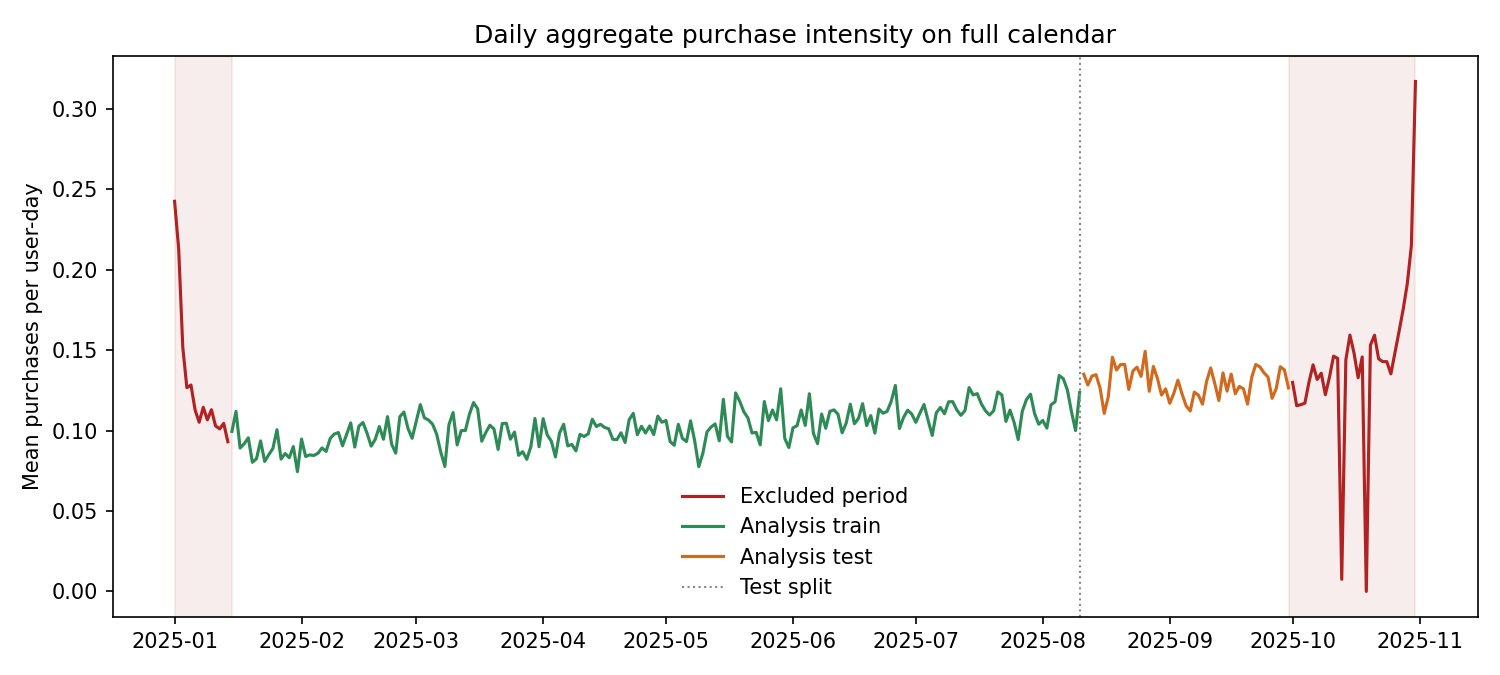
\includegraphics[width=0.85\textwidth]{images/fig02_daily_aggregate_full_ts.jpg}
\caption{Дневная интенсивность to\_ord на полном ряду}
\end{figure}


На полном ряду выделяются три режима:

\begin{enumerate}
  \item \textbf{Первые две недели января} - аномально высокая активность, связанная с послепраздничными промо-кампаниями. Среднее число покупок в этот период на \texttt{30..40\%} выше, чем в основном окне.
  \item \textbf{Период с середины января до конца сентября} - основное стабильное окно с медленным трендом и недельной сезонностью. На нём проводится большая часть экспериментов.
  \item \textbf{Октябрь} - повторное повышение уровня, связанное с предновогодними промо.
\end{enumerate}


Так как данных за прошлые года у нас, анализировать окна с сильно скачущей интенсивностью сложно. Основное окно для экспериментов фиксировано как \texttt{2025-01-15..2025-09-30}, чтобы исключить новогодний всплеск из train-данных и обеспечить стационарность фоновых характеристик. Внутри этого окна также наблюдается недельная сезонность: будни и выходные различаются по среднему уровню \texttt{to\_ord} примерно на ${±10\%}$. Эту сезонность нужно будет учесть при построение бейзлайна.

\FloatBarrier
\subsection{Гетерогенность пользователей}

Если в среднем по датасету $mean(to\_ord) \approx  0.10$, то на уровне отдельного пользователя картина может быть сильно иной. Чтобы понять, насколько активность одного пользователя предсказуема через активность того же пользователя в другом периоде, мы построили облако суммарного числа покупок на train против test для каждого пользователя (рис. 3).


\begin{figure}[ht]
\centering
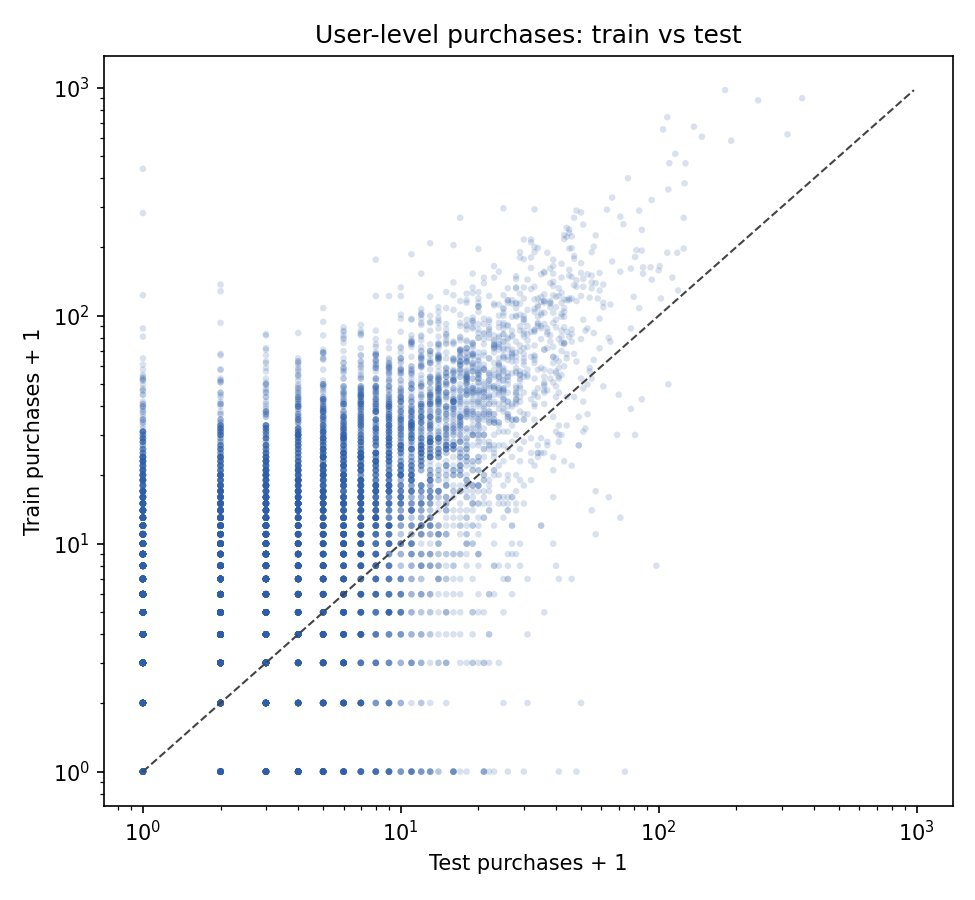
\includegraphics[width=0.85\textwidth]{images/fig03_user_train_test_scatter.jpg}
\caption{Активность пользователей: train vs test}
\end{figure}


Корреляция Пирсона между train и test суммами составляет \texttt{\textasciitilde{}0.75..0.80}. Это означает, что значительная часть будущей активности пользователя действительно предсказуема через его исторические суммы - это и есть основной сигнал для Personalized GP. Нобольшая часть дисперсии все еще остаются необъяснёнными за счёт изменения паттерна пользователя во времени, шума и редких всплесков.

В терминах модели сильное различие в поведении пользователей выражается в том, что разброс по логарифму среднего темпа $log(\mu _u)$ между пользователями составляет 2-3 порядка. Без персонализации модель неизбежно сильно недооценивает активных пользователей и переоценивает неактивных. 

Для иллюстрации структуры данных на уровне одного пользователя - пользователь 612605, активный (\texttt{321} покупка на train) - показаны его дневные счётчики по трём каналам воронки на рис. 4.


\begin{figure}[ht]
\centering
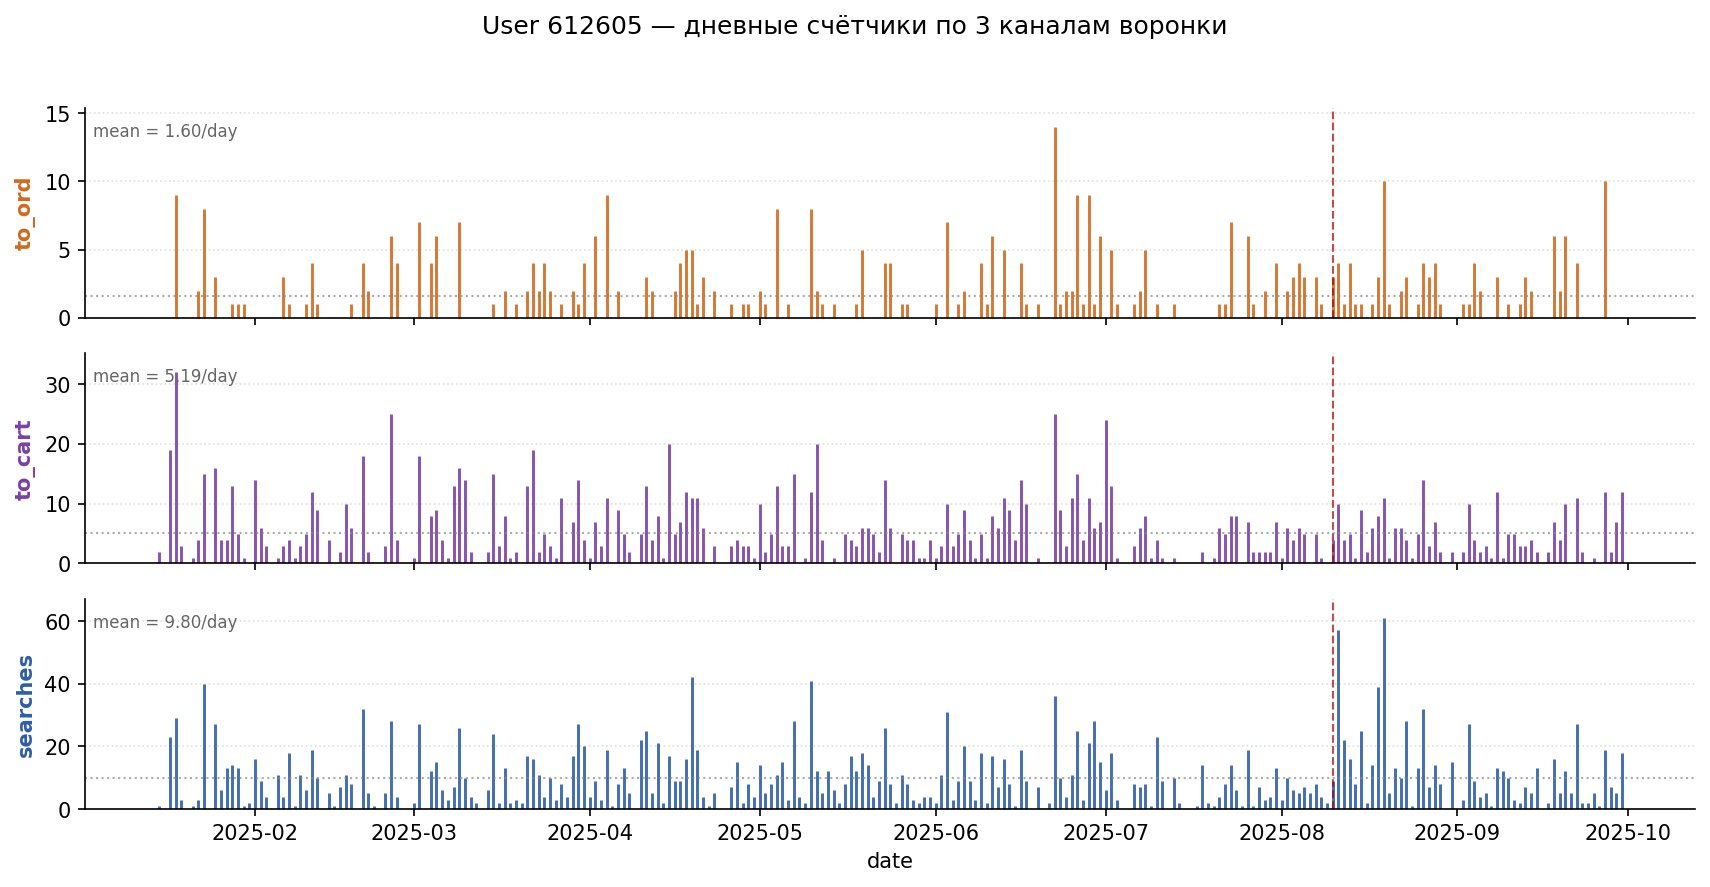
\includegraphics[width=0.85\textwidth]{images/fig04_user612605_3channels.jpg}
\caption{Счётчики пользователя 612605 по 3 каналам}
\end{figure}


На каждой панели видна экспоненциальная воронка: \texttt{searches} (mean \texttt{9.8} событий/день для этого пользователя) $\to$ \texttt{to\_cart} (\texttt{5.2}) $\to$ \texttt{to\_ord} (\texttt{1.6}). Активность нерегулярна - серии активных дней чередуются с периодами относительного затишья. Именно эту структуру self-excitation призван моделировать Hawkes.

\FloatBarrier
\subsection{Корреляции каналов и выбор признаков для Hawkes}

Матрица корреляций пяти исходных счётчиков показана на рис. 5.


\begin{figure}[ht]
\centering
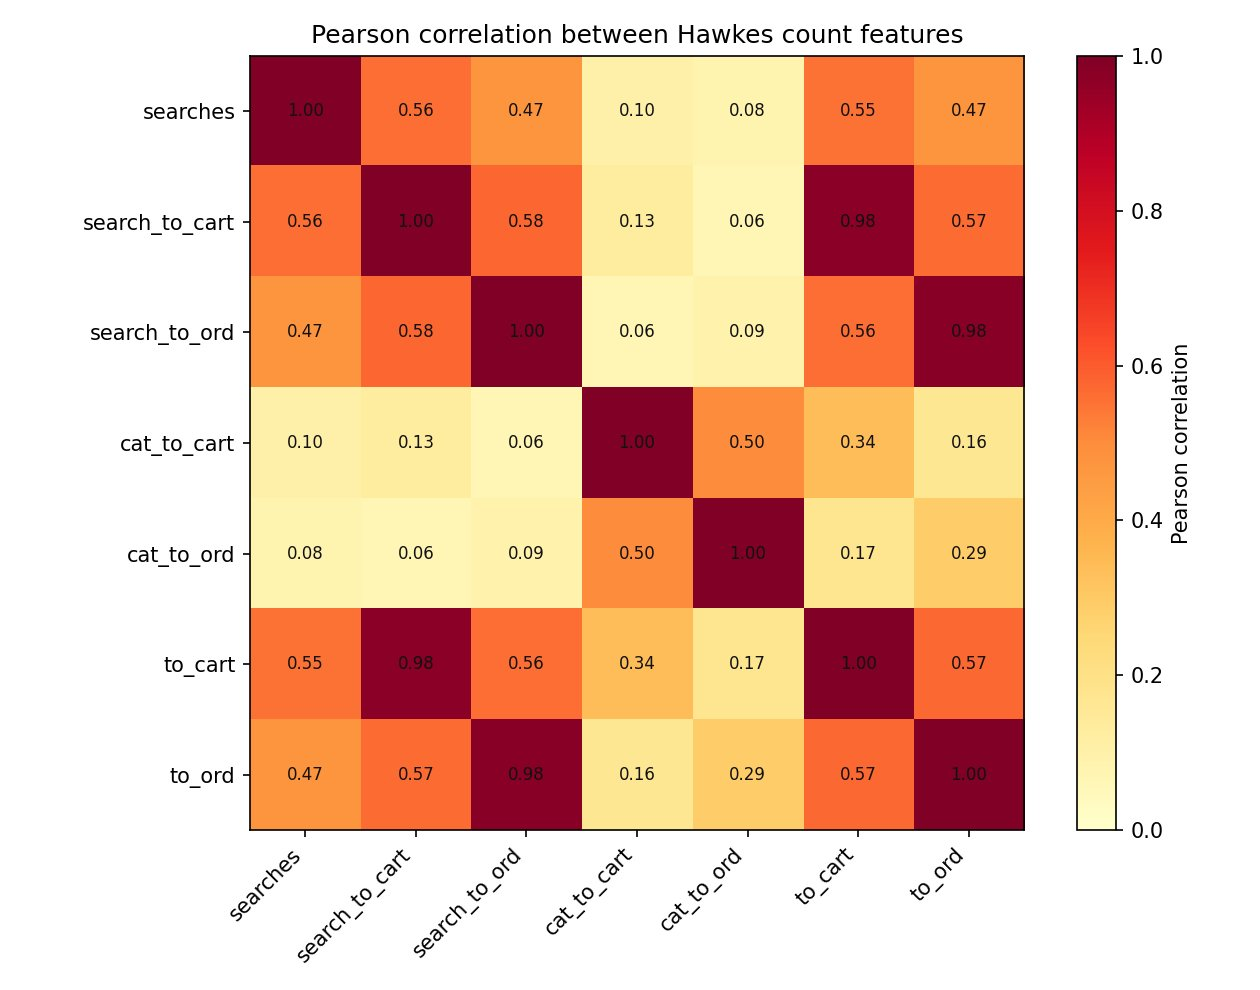
\includegraphics[width=0.85\textwidth]{images/fig05_feature_correlation_heatmap.jpg}
\caption{Корреляция исходных каналов}
\end{figure}


Каналы \texttt{search\_to\_cart} и \texttt{search\_to\_ord} сильно скоррелированы с целевыми \texttt{to\_cart} и \texttt{to\_ord} (Пирсон \texttt{r > 0.9}), поэтому их включение в Hawkes-states привело бы к коллинеарности фичей и нестабильности оценок $\alpha $. По итогам этого анализа в основной части работы мы оставляем три независимых канала: \texttt{searches}, \texttt{to\_cart}, \texttt{to\_ord}. Этого достаточно для содержательного cross-channel анализа и не приводит к мультиколлинеарности.

Корреляции между оставшимися тремя каналами умеренные ($r \approx  0.3..0.5$), что и должно быть для каналов воронки: события вышестоящих этапов (\texttt{searches}) частично, но не полностью предсказывают события нижестоящих (\texttt{to\_ord}).

\FloatBarrier
\subsection{Метрика качества: per-observation Poisson NLL и saturated floor}

Основная скоринговая метрика - средний негативный log-likelihood Пуассоновской модели на одну строку датасета:

\[
\mathrm{NLL} \;=\; \frac{1}{N} \sum_{u,t} \Big[\, \lambda_{u,t} \;-\; y_{u,t} \log \lambda_{u,t} \;+\; \log y_{u,t}! \,\Big].
\]

Чем меньше - тем лучше. Метрика согласована с самой моделью наблюдения и поэтому используется как primary criterion при сравнении моделей. Дополнительно для диагностики и сопоставимости с регрессионными моделями (бустинг) используются MAE и RMSE.

Существует теоретический минимум NLL, недостижимый никакой Пуассоновской моделью: \textbf{saturated Poisson floor}, получаемый подстановкой $\lambda _i = y\_i$ в каждой строке. Действительно, при фиксированном \texttt{y} функция $\lambda  -> \log p(y \mid \lambda )$ достигает максимума при $\lambda  = y$, поэтому

\[
\mathrm{LL}_{\mathrm{sat}} \;=\; \sum_{i} \Big( y_i \log y_i - y_i - \log(y_i!) \Big),
\]

с договорённостью \texttt{0 log 0 := 0}. На нашем test-окне ($N \approx  513K$ строк) saturated floor $NLL\_sat \approx  0.0862$. Это абсолютный нижний предел: разница между лучшей нашей моделью и этим floor'ом - это та часть aleatoric uncertainty, которую никаким Пуассоновским предсказанием закрыть нельзя.

Связь saturated floor'а с deviance даёт удобный способ оценивать его из уже обученной модели: \texttt{NLL\_\{model\} - NLL\_\{sat\} = mean Deviance / 2}. Мы используем это соотношение в коде для проверки численной согласованности разных экспериментов.

\clearpage
\section{Часть I. Бейзлайн и Хоукс-надстройка на полном train-test}

В этой части мы поэтапно строим модель интенсивности $\lambda _{u,t}$. Сначала собираем сильный пуассоновский бейзлайн и обосновываем, какой именно его вариант лучше всего подходит как основа для Хоукс-надстройки. Затем строим саму Хоукс-надстройку и измеряем её вклад. Отдельно рассматриваем бустинг как control-модель, дающую верхнюю планку качества. В конце сводим все полученные модели в единую лестницу и сравниваем по нескольким метрикам. Все эксперименты этой части - на основном протоколе: train \texttt{207d}, test \texttt{52d}.

\FloatBarrier
\subsection{Постановка: зачем нужен сильный бейзлайн}

Напомним постановку из раздела 1.2: в дискретной форме интенсивность раскладывается на бейзлайн и Хоукс-надстройку,

\[
\lambda_{u,t} \;=\; \underbrace{\mu_{u,t}}_{\text{бейзлайн}} \;+\; \underbrace{\sum_{j} \alpha_j \cdot z_{u,j,t}}_{\text{Хоукс-надстройка}}.
\]

Чтобы честно измерить вклад Хоукс-части, нужен максимально сильный бейзлайн $\mu _{u,t}$. Иначе любое улучшение от Хоукс-надстройки рискует объясняться тем, что бейзлайн просто плохо ловит ту часть сигнала, которую сами события могли бы объяснить и без явной self-excitation структуры. Поэтому в Части I сначала строим бейзлайн поэтапно - от простейшего «единая константа» до Personalized Gamma-Poisson с байесовской регуляризацией per-user множителя, - и только после этого добавляем над ним Хоукс-надстройку.

\FloatBarrier
\subsection{Построение бейзлайна}

Бейзлайн строится поэтапно - сначала несколько простых уровней без персонализации, потом полноценная пользовательская модель:

\begin{enumerate}
  \item \textbf{Global Poisson} - единая константа $\bar{\lambda}$ на весь датасет. Самая простая модель; даёт точку отсчёта.
  \item \textbf{Rolling Poisson} - скользящее среднее дневного уровня по предыдущим дням. Добавляет учёт глобального тренда без персонализации.
  \item \textbf{Rolling Seasonal Poisson} - Rolling с поправкой на день недели. Учитывает недельную сезонность (будни vs выходные).
  \item \textbf{Personalized Gamma-Poisson} - переход от общего дневного профиля к модели с индивидуальным множителем $\mu _u$ для каждого пользователя. Эта модель станет финальным бейзлайном для Хоукс-надстройки.
\end{enumerate}


На нашем протоколе первые три модели различаются между собой слабо (test NLL \texttt{0.4608 → 0.4576 → 0.4576}): разброс активности между пользователями кратно превышает изменчивость дневного среднего и недельной сезонности. Большой шаг - это переход к персонализации, дающий test NLL \texttt{0.4096} (выигрыш \texttt{+24K} в LL над Global Poisson). Ниже подробно разбираем именно Personalized GP как опорный бейзлайн для всех Хоукс-моделей.

\textbf{Идея персонализации.} Дневной профиль $b\_t$ из Rolling Seasonal даёт хорошее общее представление об уровне активности по когорте, но не отличает активного пользователя от неактивного. Естественный способ это исправить - домножить общий профиль на индивидуальный коэффициент $\mu _u$:

\[
\lambda_{u,t} \;=\; \mu_u \cdot b_t.
\]

Если бы у каждого пользователя было много данных, $\mu _u$ можно было бы оценить простым MLE: $\hat\mu _u = Y\_u / E\_u$, где $Y\_u = \sum_t y_{u,t}$ - суммарное число покупок пользователя на train, а $E\_u = \sum_t b\_t$ - суммарная экспозиция. Но в нашей задаче для большинства пользователей $Y\_u$ маленькое (0-2 покупки на train), и MLE-оценка получается крайне неустойчивой: один лишний наблюдённый день меняет $\hat\mu _u$ в разы. В крайнем случае при $Y\_u = 0$ MLE даёт $\hat\mu _u = 0$, что приводит к нулевому прогнозу интенсивности и взрыву NLL на любом ненулевом дне теста.

Поэтому персонализацию в чистом виде применять нельзя - нужна регуляризация: малоактивные пользователи, про которых известно мало, должны автоматически подтягиваться к когортному уровню, а активные с достаточным количеством данных - оставаться близко к своей MLE-оценке.

\textbf{Полный байесовский вывод.} Модель достаточно простая, чтобы вместо явного штрафа провести регуляризацию через полный байесовский вывод. Кладём на $\mu _u$ Gamma-prior со средним $\approx 1$ - то есть выражаем априорное представление о том, что средний пользователь имеет множитель около единицы:

\[
y_{u,t} \mid \mu_u \sim \mathrm{Poisson}(\mu_u \cdot b_t), \qquad \mu_u \sim \mathrm{Gamma}(\alpha, \beta).
\]

Благодаря сопряжённости Gamma и Poisson posterior $\mu _u$ тоже распределён по Gamma и выписывается в замкнутой форме:

\[
\mu_u \mid Y_u, E_u \sim \mathrm{Gamma}(\alpha + Y_u, \beta + E_u).
\]

В качестве точечной оценки берём posterior mean:

\[
\hat\mu_u^{\mathrm{EB}} \;=\; \frac{\alpha + Y_u}{\beta + E_u}.
\]

В этом выражении видно, как байесовский вывод сам решает задачу регуляризации. Для пользователя, про которого мало данных ($Y\_u \approx 0$, $E\_u$ маленькое), оценка сводится к $\alpha / \beta \approx 1$ - то есть к среднему по когорте. Для активного пользователя с большим $Y\_u$ влияние prior'а становится пренебрежимо малым, и $\hat\mu _u^{\mathrm{EB}} \to Y\_u / E\_u$, то есть к обычному MLE. Никакого дополнительного гиперпараметра «силы регуляризации» здесь нет - баланс между prior'ом и данными выставляется автоматически в зависимости от того, сколько информации есть про конкретного пользователя.

\textbf{Оценка гиперпараметров.} Параметры $(\alpha , \beta )$ prior'а оцениваются эмпирически - по marginal MLE по всем \texttt{\textasciitilde{}10K} пользователям одновременно (Empirical Bayes). Интегрируя $\mu _u$, получаем маргинальное распределение $(Y\_u, E\_u)$ - отрицательное биномиальное, и минимизируем суммарный $-\log p(Y\_u, E\_u \mid \alpha , \beta )$ по $(\alpha , \beta )$ методом L-BFGS-B. На нашем датасете это даёт $(\alpha , \beta ) \approx (0.88, 0.88)$ - то есть prior со средним $\approx 1$, что согласуется с интерпретацией «средний пользователь имеет множитель около единицы».

Без байесовской регуляризации (чистая MLE с обрезкой $\mu _u = 0$ при $Y\_u = 0$) test NLL на полном \texttt{52d}-test составляет \texttt{0.4650}. Полный байесовский вывод даёт \texttt{0.4096} - выигрыш порядка \texttt{+24K} в LL. Это и есть основное улучшение на пути к опорному бейзлайну.

Анализ выигрыша на уровне отдельных пользователей через \textbf{per-user delta-LL} даёт следующую картину (рис. 6):


\begin{figure}[ht]
\centering
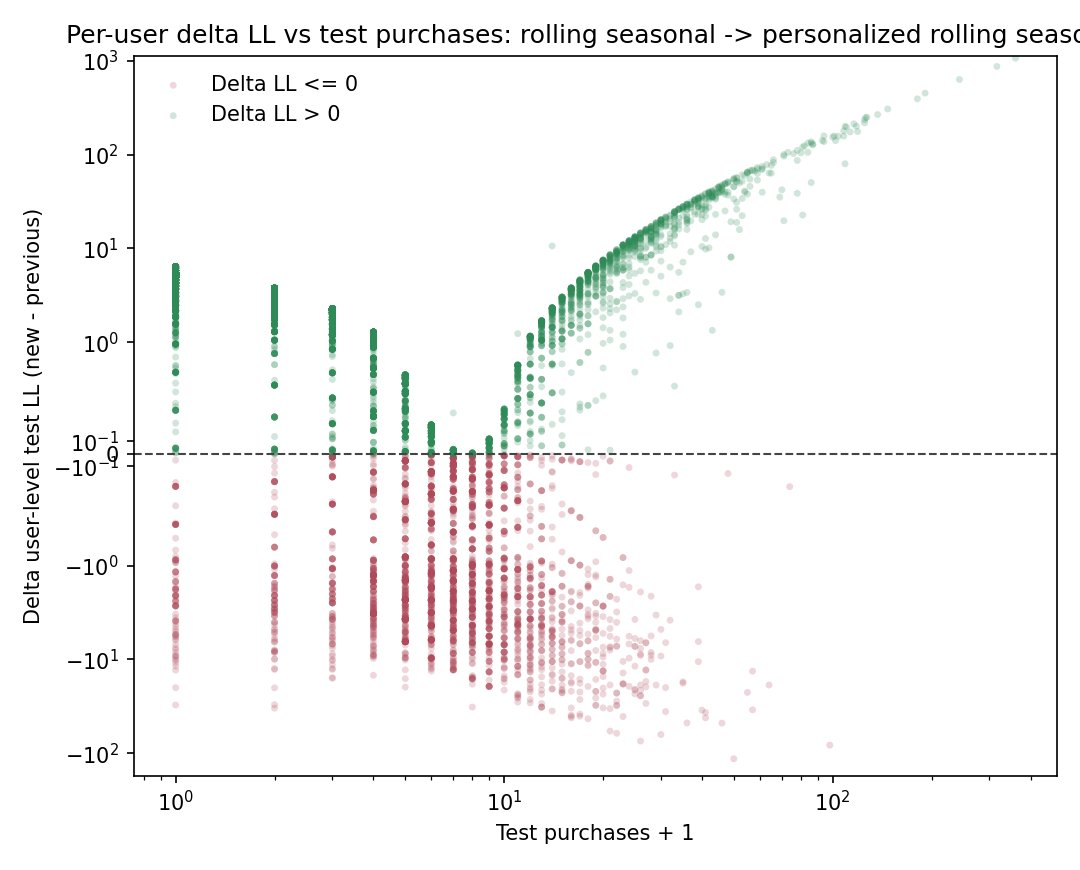
\includegraphics[width=0.85\textwidth]{images/fig08_delta_ll_vs_test_purchases_rolling_seasonal_to_personalized.jpg}
\caption{Per-user delta-LL: Rolling Seasonal → Personalized}
\end{figure}


Распределение \texttt{ΔLL = LL\_\{PersGP\} - LL\_\{RS\}} по пользователям сильно неоднородно:

\begin{itemize}
  \item \texttt{share(personalized > rolling seasonal) = 66\%} - две трети пользователей выигрывают от персонализации.
  \item Юзеры с \texttt{0..2} покупками выигрывают почти всегда (\texttt{87..94\%}) - для них Personalized GP правильно сдвигает прогноз вниз от среднего по когорте.
  \item Бакет \texttt{6..10} покупок - наоборот, проигрывает (\texttt{18\%}): на этих пользователях регуляризация ещё ощутимо тянет к когортному среднему, и чистая MLE сработала бы лучше.
  \item Активные с \texttt{11+} снова выигрывают, потому что $\hat\mu _u^{\mathrm{EB}}$ на них почти не отличается от MLE.
\end{itemize}


Это структурное замечание важно для интерпретации Хоукс-результатов: Хоукс-надстройка будет работать поверх уже регуляризованного персонализированного бейзлайна и сможет компенсировать чрезмерную регуляризацию на активной части когорты.

\FloatBarrier
\subsection{Scaled-baseline Hawkes на персонализированной базе}

Над Personalized Gamma-Poisson бейзлайном мы строим \textbf{Scaled-baseline Hawkes} - модель с фиксированной персонализированной базой и pooled Хоукс-надстройкой:

\[
\lambda_{u,t} \;=\; c \cdot \mu_u^{\mathrm{EB}} \cdot b_t \;+\; \sum_{j,m} \alpha_{j,m} \cdot z_{u,j,m,t},
\]

где \texttt{c} - глобальный масштаб базы (один скаляр на всю когорту), а \texttt{z\_\{u,j,m,t\}} - Hawkes-state с полураспадом \texttt{m} для фичи \texttt{j}. В основной реализации мы используем 5 фичей $\times$ 2 полураспада \texttt{(1, 3)} дня, что даёт 10 параметров $\alpha $ и один скаляр \texttt{c} - итого 11 обучаемых параметров плюс per-user multiplier'ы ($\approx$10K) из EB-шага.

Обучение двухступенчатое (staged):

\begin{enumerate}
  \item \textbf{EB-шаг} (наследуется из бейзлайна): из Personalized GP получены $\mu _u^{EB}$, $(\alpha , \beta )$ и \texttt{b\_t}. На этом шаге per-user multiplier'ы зафиксированы.
  \item \textbf{Хоукс-шаг}: численная оптимизация $(c, \alpha )$ методом L-BFGS-B с ограничением $\alpha  \geq  0$. Loss - Пуассоновский негативный log-likelihood с мягкой L2-регуляризацией:
\end{enumerate}


\[
\mathcal{L}(c, \alpha) \;=\; -\log p\!\left(y \mid c \lambda_{\mathrm{base}} + X\alpha\right) \;+\; \lambda_\alpha \|\alpha\|_2^2 \;+\; \lambda_c (c - 1)^2.
\]

Ограничением гарантируют, что Хоукс-надстройка не может стать отрицательной (что нарушило бы Пуассоновскую интерпретацию $\lambda  \geq  0$). На каждой итерации L-BFGS-B градиент по $(c, \alpha )$ считается аналитически из chain rule, что делает фит быстрым: на 11 параметрах и \texttt{\textasciitilde{}2M} строк сходимость достигается за \texttt{\textasciitilde{}100..300} итераций (\texttt{\textasciitilde{}30} секунд на CPU).

На главном \texttt{207d}-train Scaled Hawkes даёт test NLL \texttt{0.3958} против \texttt{0.4096} у Pers GP - улучшение \texttt{+7K} в LL, или \texttt{-0.014} в NLL. Обученные параметры: $\hat{c} \approx  0.83$, $\|\alpha \|_2 \approx  0.016$. Тот факт, что \texttt{c < 1}, говорит о том, что оптимизатор слегка уменьшает фоновую часть, компенсируя её Хоукс-надстройкой. Это первый намёк на то, что между $c \cdot  \mu _u$ и Hawkes-states существует trade-off, к которому мы вернёмся в части III.

Обученная матрица $\alpha [feature \times  half-life]$ визуализируется на рис. 7. Основной вклад приходится на \texttt{to\_ord (hl=3)} - наибольший положительный коэффициент, отражающий, что недавняя покупка действительно повышает интенсивность следующей покупки в течение 3 дней. Также видны положительные $\alpha $ для \texttt{searches} и \texttt{to\_cart} на масштабе 1 день, что соответствует короткой воронке \texttt{search → cart → order} в пределах одной-двух сессий пользователя.


\begin{figure}[ht]
\centering
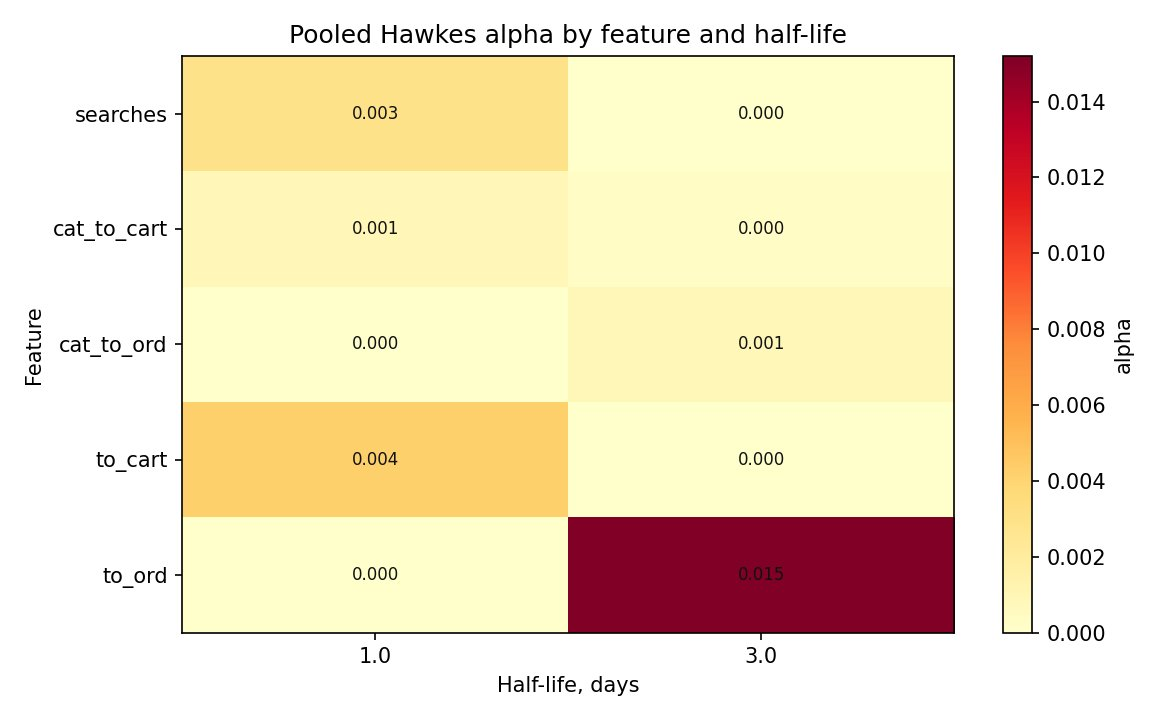
\includegraphics[width=0.85\textwidth]{images/fig09_alpha_heatmap.jpg}
\caption{Тепловая карта Хоукс-коэффициентов: feature × half-life (Scaled Hawkes)}
\end{figure}


Анализ per-user delta-LL (рис. 8) показывает, что Хоукс-надстройка даёт выигрыш у \texttt{63.4\%} пользователей. В отличие от перехода к персонализации, выигрыш распределён более равномерно по всем бакетам активности (\texttt{54..80\%} пользователей выигрывают в каждом бакете). Это говорит о том, что Хоукс-сигнал работает поверх уже выровненного персонализированного бейзлайна и не страдает от перекосов регуляризации.


\begin{figure}[ht]
\centering
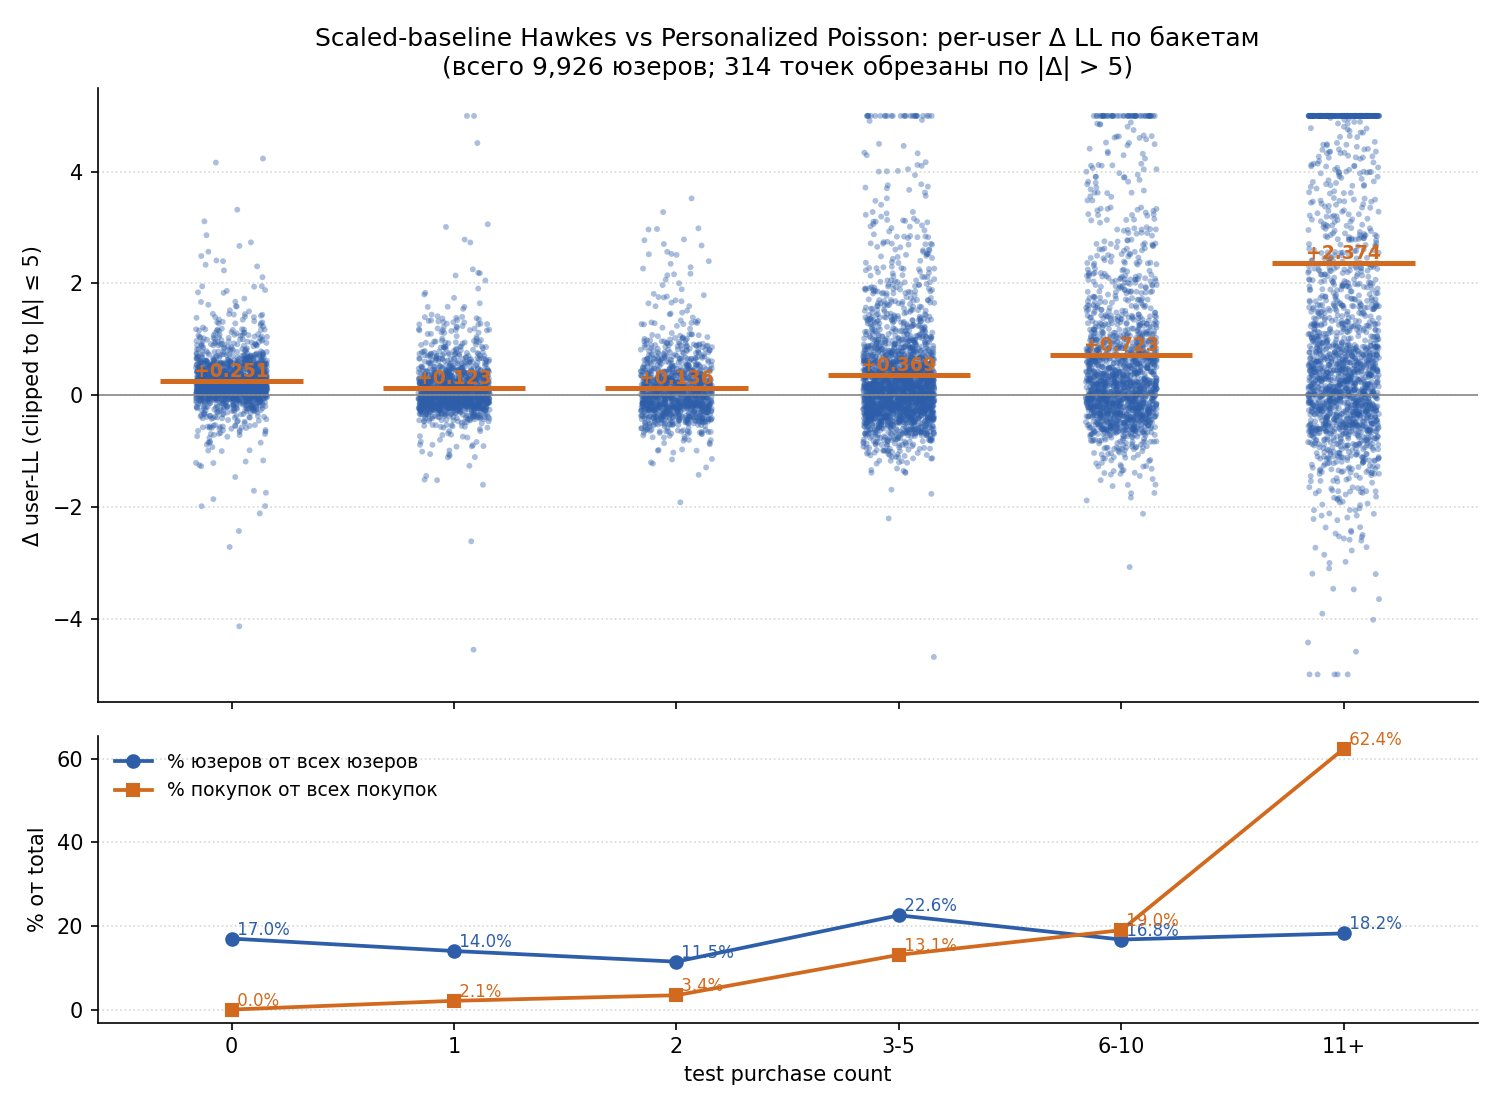
\includegraphics[width=0.85\textwidth]{images/fig10_delta_ll_vs_test_purchases_personalized_to_hawkes.jpg}
\caption{Per-user delta-LL: Personalized → Scaled Hawkes}
\end{figure}


Mean / median delta-LL: \texttt{+0.71} / \texttt{+0.16} на пользователя. Это значит, что среднее улучшение скромное, но устойчивое - нет хвоста пользователей, на которых Hawkes резко проигрывает бейзлайну. Это критичное практическое свойство: модель надёжна на всей когорте.

\textbf{Регуляризация и выбор полураспадов.} Для модели на 11 параметрах с \texttt{\textasciitilde{}2M} строк train regularization-сетка $(\lambda _\alpha , \lambda _c) \in  \{0, 0.01, 0.1, 1, 10, 100\}^2$ показывает, что результат \textbf{не зависит от регуляризации в широком диапазоне}: размах test NLL по всей сетке составляет менее \texttt{0.0005}. Это согласуется с практическим правилом, что при \texttt{(n\_obs / n\_params) > 10\textasciicircum{}5} явная регуляризация почти не влияет на оптимум - данных достаточно, чтобы оценить параметры с малой дисперсией без помощи prior'а.

Выбор полураспадов - отдельный методический вопрос. Мы тестировали значения $\tau  \in  \{0.5, 1, 2, 3, 5, 7\}$ дня в комбинации с разным числом параллельных ядер. Главные наблюдения:

\begin{itemize}
  \item Один полураспад $\tau  = 1$ день даёт самый простой и быстрый фит, но теряет недельный «хвост» активности.
  \item Комбинация \texttt{(1, 3)} дня даёт оптимум по test NLL и сохраняет интерпретируемость двух разделённых масштабов памяти: «немедленный» (сегодня $\to$ завтра) и «среднесрочный» (3-дневная сессия).
  \item Дополнительный третий полураспад $\tau  = 7$ дней не улучшает скор: его профиль NLL почти плоский. Это значит, что longer-term память уже захвачена бейзлайном $b\_t \cdot  \mu _u$ через rolling-агрегацию.
  \item Полураспады меньше суток ($\tau  < 1$) теряют смысл для дневной агрегации: они не отличают «сегодня» от «вчера».
\end{itemize}


В дальнейшем в работе используется конфигурация \texttt{(1, 3)} дня для всех Хоукс-моделей.

\FloatBarrier
\subsection{Joint Hawkes как альтернативная параметризация}

Рядом со Scaled-baseline Hawkes мы вводим вторую Хоукс-параметризацию - \textbf{Joint Hawkes}, где per-user множители $\lambda _u$ и коэффициенты $\alpha $ обучаются \textbf{совместно} напрямую через MLE с явной L2-регуляризацией:

\[
\lambda_{u,t} \;=\; \lambda_u \cdot b_t \;+\; \alpha^{\top} z_{u,t}, \qquad \mathcal{L} \;=\; \mathrm{NLL}(y, \lambda) \;+\; \lambda_{\ell_2} \sum_u (\lambda_u - 1)^2 \;+\; \lambda_\alpha \|\alpha\|_2^2.
\]

Главные отличия от Scaled-baseline:

\begin{itemize}
  \item \textbf{Одностадийное обучение} - без отдельного EB-шага. Empirical-Bayes prior на $\mu _u$ заменён явным L2-prior'ом $(\lambda _u - 1)^2$, и оптимизатор учитывает его одновременно с Хоукс-частью.
  \item \textbf{$\lambda _u$ обучается напрямую}, а не наследуется зафиксированным из бейзлайна. Это даёт оптимизатору свободу «перекинуть» массу интенсивности между $\lambda _u$ и Хоукс-вкладом - Scaled-baseline такой возможности не имеет, потому что $\mu _u^{EB}$ зафиксирован.
\end{itemize}


Обучение - L-BFGS-B по $(n_{\text{users}} + n_\alpha ) \approx 10010$ параметрам; благодаря разреженности градиента сходится за \texttt{\textasciitilde{}400..600} итераций (\texttt{\textasciitilde{}60..120} секунд на CPU). По умолчанию фиксируем $\lambda _{\ell_2} = 1$ как «активный prior».

На главном \texttt{207d}-train Joint Hawkes даёт почти то же качество, что и Scaled-baseline (test NLL \texttt{0.3951} vs \texttt{0.3958}) - по NLL модели на полном объёме данных практически неотличимы. Но \textbf{структура регуляризации у них принципиально разная}, и за счёт этого на коротких train-окнах они выучивают разные закономерности и приходят к разным точкам в пространстве параметров. Это явление детально разбираем в Части II.

\FloatBarrier
\subsection{Бустинг и feature engineering}

Чтобы сравнение Хоукс-моделей с бустингом было объективным, бустинг мы тоже старались максимально вытянуть. Основной рычаг улучшения оказался со стороны \textbf{feature engineering}: из 5 исходных поведенческих счётчиков (\texttt{searches}, \texttt{cat\_to\_cart}, \texttt{cat\_to\_ord}, \texttt{to\_cart}, \texttt{to\_ord}) и нескольких производных каналов мы построили \textbf{141 фичу}, покрывающую историю, тренды, EMA, recency и funnel-ratio. Конкретный набор признаков можно сгруппировать:

\begin{itemize}
  \item \textbf{Календарные} (3): \texttt{dow}, \texttt{days\_seen}, \texttt{week\_idx}.
  \item \textbf{History по каждому source-каналу} (14 $\times$ 8 = 112): \texttt{*\_yesterday}, \texttt{*\_sum3}, \texttt{*\_sum7}, \texttt{*\_mean7}, \texttt{*\_active\_days7}, \texttt{*\_exp3}, \texttt{*\_last\_active}, \texttt{*\_days\_since\_last\_active}.
  \item \textbf{Агрегаты по заказам и активности}: \texttt{orders\_hist\_mean}, \texttt{carts\_hist\_mean}, \texttt{any\_activity\_sum7}, \texttt{any\_activity\_mean7} и т.п.
  \item \textbf{EMA}: \texttt{to\_ord\_ewm7}, \texttt{to\_ord\_ewm28}, \texttt{to\_ord\_ewm\_gap\_7\_28}, \texttt{to\_cart\_ewm7}, \texttt{to\_cart\_ewm28}, \texttt{any\_activity\_ewm7}, \texttt{any\_activity\_ewm28}.
  \item \textbf{Recency и funnel-ratio}: \texttt{days\_since\_last\_*}, \texttt{ord\_per\_cart\_7}, \texttt{search\_to\_cart\_rate\_7}, \texttt{search\_to\_ord\_rate\_7}, \texttt{cat\_to\_cart\_rate\_7}, \texttt{cat\_to\_ord\_rate\_7}.
\end{itemize}


В качестве модели используем \texttt{HistGradientBoostingRegressor} с Poisson loss. Финальные гиперпараметры: \texttt{max\_iter=200}, \texttt{max\_depth=5}, \texttt{learning\_rate=0.05}, \texttt{min\_samples\_leaf=40}, early stopping по held-out fraction. Со стороны гиперпараметров мы провели несколько точечных экспериментов (вариации глубины, learning rate, числа итераций), но заметного отклика по NLL они не дали - в итоге зафиксировали усреднённо-разумную конфигурацию без агрессивного тюнинга.

Test NLL бустинга - \texttt{0.3881}, что лучше Scaled-baseline Hawkes (\texttt{0.3958}). Выигрыш составляет \texttt{+3K..7K} в LL. Это означает две вещи. Во-первых, GBDT действительно ловит дополнительный сигнал, которого нет в Hawkes - главным образом нелинейные взаимодействия между фичами recency и активностью. Во-вторых, его абсолютная улучшайка относительно Hawkes мала по сравнению с разрывом между Hawkes и теоретическим saturated floor (\texttt{0.0862}): большая часть оставшегося потенциала - это внутренний шум данных.

В работе GBDT отмечается отдельным цветом - как \textbf{reference point}, дающий верхнюю планку качества. Цель - оценить, на каком расстоянии от этой планки находятся интерпретируемые Хоукс-модели.

\FloatBarrier
\subsection{Итоговая лестница моделей}

Соберём все рассмотренные модели в единую сводную картину. Получается лестница из шести вероятностных моделей плюс GBDT и теоретический saturated floor:

\begin{enumerate}
  \item \textbf{Global Poisson} - единая константа $\bar{\lambda}$ на весь датасет.
  \item \textbf{Rolling Poisson} - скользящее среднее дневного уровня, без персонализации.
  \item \textbf{Rolling Seasonal Poisson} - с поправкой на день недели.
  \item \textbf{Personalized Gamma-Poisson} - персонализация множителем $\mu _u$ на предыдущю модель через Байесовский вывод.
  \item \textbf{Scaled-baseline Hawkes} - Personalized GP с Хоукс-надстройкой.
  \item \textbf{Joint Hawkes} - совместная оптимизация $\lambda _u$ и $\alpha $ напрямую через MLE с L2-prior'ом (см. подсекцию выше).
  \item \textbf{GBDT} - control-модель на расширенном feature-engineering'е (см. предыдущую подсекцию).
\end{enumerate}


Каждый следующий уровень включает в себя структуру предыдущего и добавляет один концептуальный шаг.

Главный вывод: самый крупный единичный шаг - переход к \textbf{персонализации} (Gamma-Poisson, \texttt{-0.0480} в NLL). Все четыре «не персонализированных» бейзлайна на полной кривой почти не отличаются друг от друга, поскольку разброс между пользователями кратно превышает изменчивость во времени. Следующий заметный шаг - Хоукс-надстройка (\texttt{-0.0138} в NLL). Joint Hawkes даёт почти то же значение, что и Scaled-baseline, отличаясь от него на \texttt{-0.0007} в NLL - это уже на уровне численного шума. GBDT снимает ещё \texttt{-0.0070} в NLL, занимая верхнюю планку.

Численная таблица:


\begin{table}[ht]
\centering
\small
\begin{tabular}{rlrrr}
\toprule
Ступень & Модель & Test LL & NLL/n & $\Delta$ vs предыдущая (NLL) \\
\midrule
1 & Global Poisson & \texttt{-236458} & \texttt{0.4608} & - \\
2 & Rolling Poisson & \texttt{-234805} & \texttt{0.4576} & \texttt{-0.0032} \\
3 & Rolling Seasonal & \texttt{-234782} & \texttt{0.4576} & \texttt{-0.0000} \\
4 & Personalized Gamma-Poisson & \texttt{-210167} & \texttt{0.4096} & \texttt{-0.0480} \\
5 & Scaled-baseline Hawkes & \texttt{-203093} & \texttt{0.3958} & \texttt{-0.0138} \\
6 & Joint Hawkes ($\lambda _u + \alpha $) & \texttt{-202721} & \texttt{0.3951} & \texttt{-0.0007} \\
7 & GBDT (experimental) & \texttt{-199154} & \texttt{0.3881} & \texttt{-0.0070} \\
- & Saturated Poisson floor & \texttt{-44216} & \texttt{0.0862} & - \\
\bottomrule
\end{tabular}
\end{table}


Доля закрытого зазора между Global Poisson и saturated floor'ом, накопленная к Joint Hawkes, составляет \texttt{\textasciitilde{}18\%}; до GBDT - \texttt{\textasciitilde{}19\%}. Остающиеся \texttt{\textasciitilde{}80\%} - это внутренний шум данных, который не может быть закрыт никаким Пуассоновским предсказанием на текущих признаках.

Сводная картина моделей по per-observation NLL и LL/RMSE приведена на рис. 9 и 10.


\begin{figure}[ht]
\centering
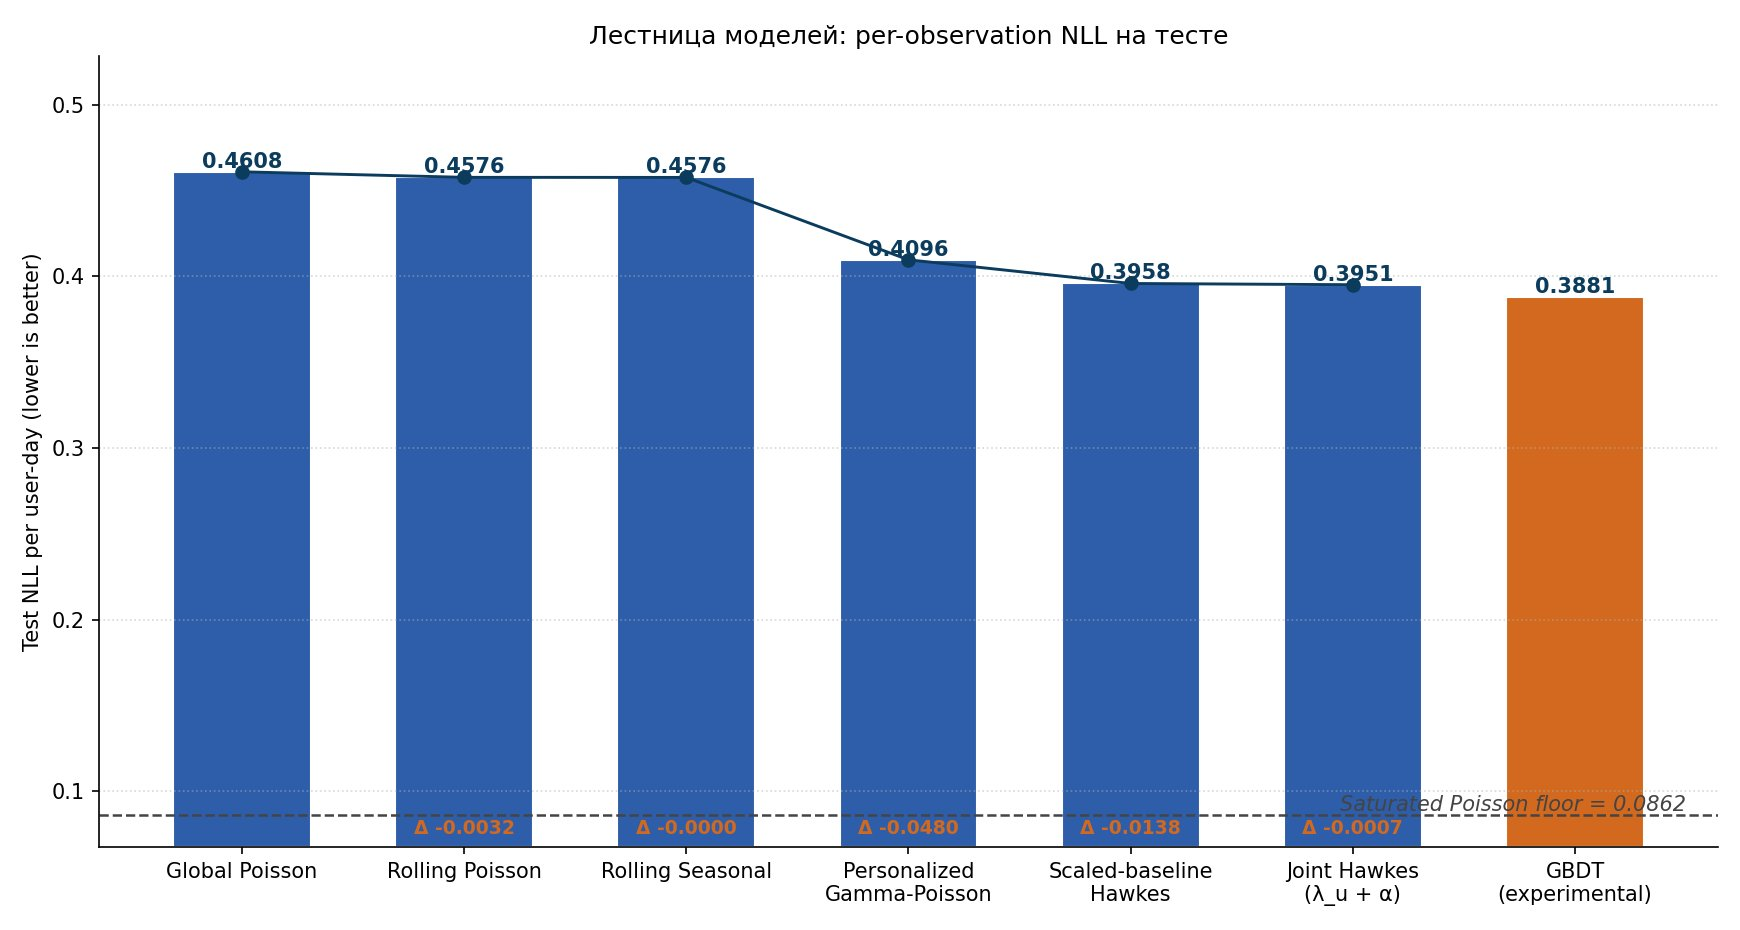
\includegraphics[width=0.85\textwidth]{images/fig11_test_nll_per_obs_ladder.jpg}
\caption{Per-observation NLL: лестница моделей}
\end{figure}


\begin{figure}[ht]
\centering
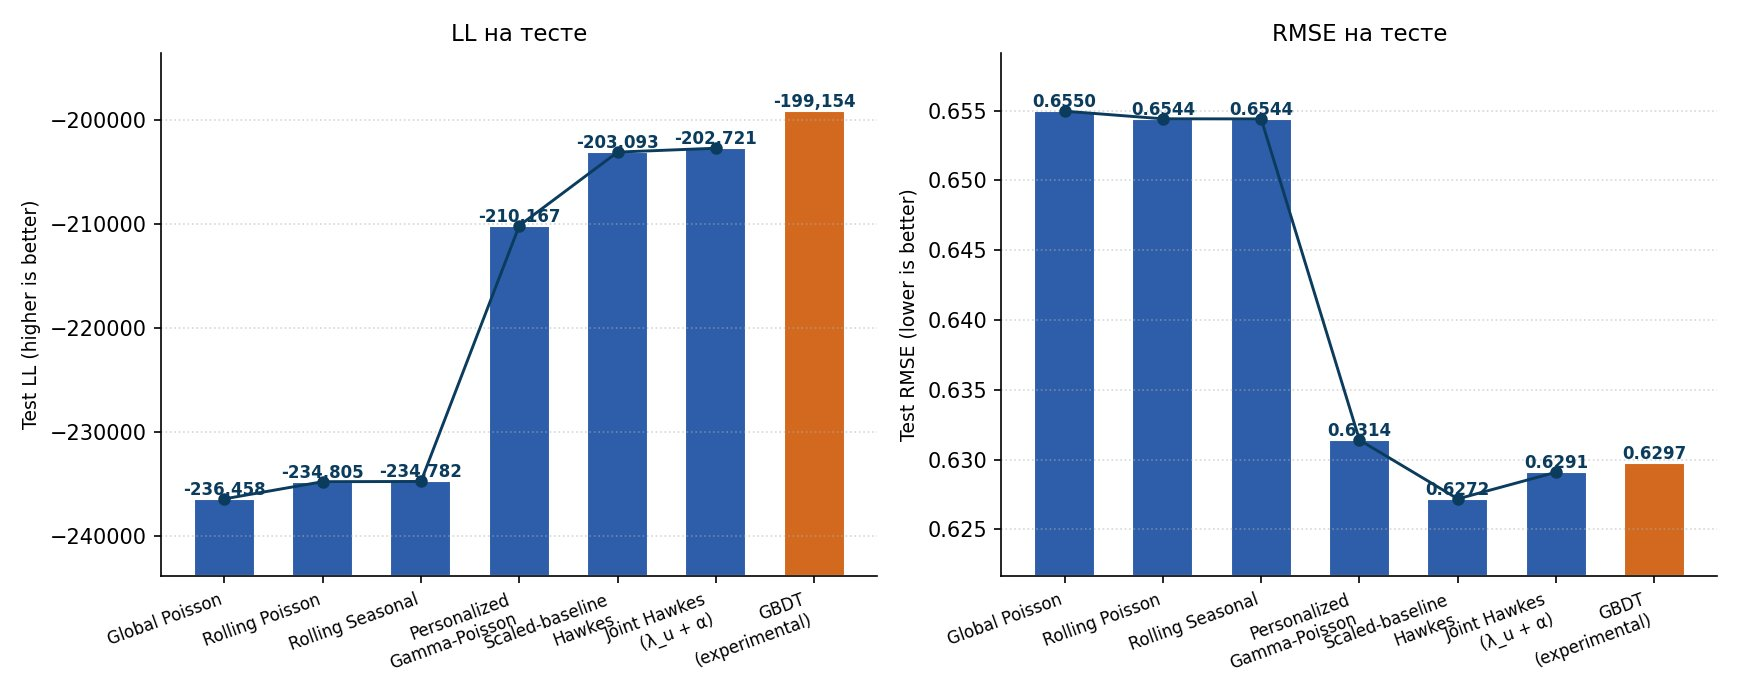
\includegraphics[width=0.85\textwidth]{images/fig12_test_ll_rmse_ladder.jpg}
\caption{Test LL и RMSE по моделям}
\end{figure}


Видно, что:

\begin{itemize}
  \item Крупный шаг по NLL даёт переход к персонализации.
  \item Хоукс-надстройка добавляет ещё стабильный шаг порядка \texttt{0.014} в NLL.
  \item Между Scaled-baseline и Joint Hawkes разница ничтожна (\texttt{0.0007} в NLL).
  \item GBDT обходит все вероятностные модели, но без интерпретируемой структуры.
\end{itemize}


LL-чарт повторяет ту же лестницу в абсолютных числах: переход к персонализации даёт скачок порядка \texttt{+24K} в LL, Хоукс-надстройка - ещё \texttt{+7K}, GBDT улучшает Joint Hawkes ещё на \texttt{+3.6K}. RMSE даёт более согласованную с NLL картину, монотонно убывая от бейзлайна к Hawkes (\texttt{0.655 → 0.627}); GBDT практически совпадает с Joint Hawkes по RMSE (\texttt{0.6297} vs \texttt{0.6291}).

Интересный диагностический график - scatter обученных per-user multiplier'ов: \texttt{m\_u} из Scaled-baseline Hawkes (где $m\_u = c \cdot  \mu _u^{EB}$) против \texttt{m\_u} из Joint Hawkes (где $m\_u = \lambda _u$ напрямую).


\begin{figure}[ht]
\centering
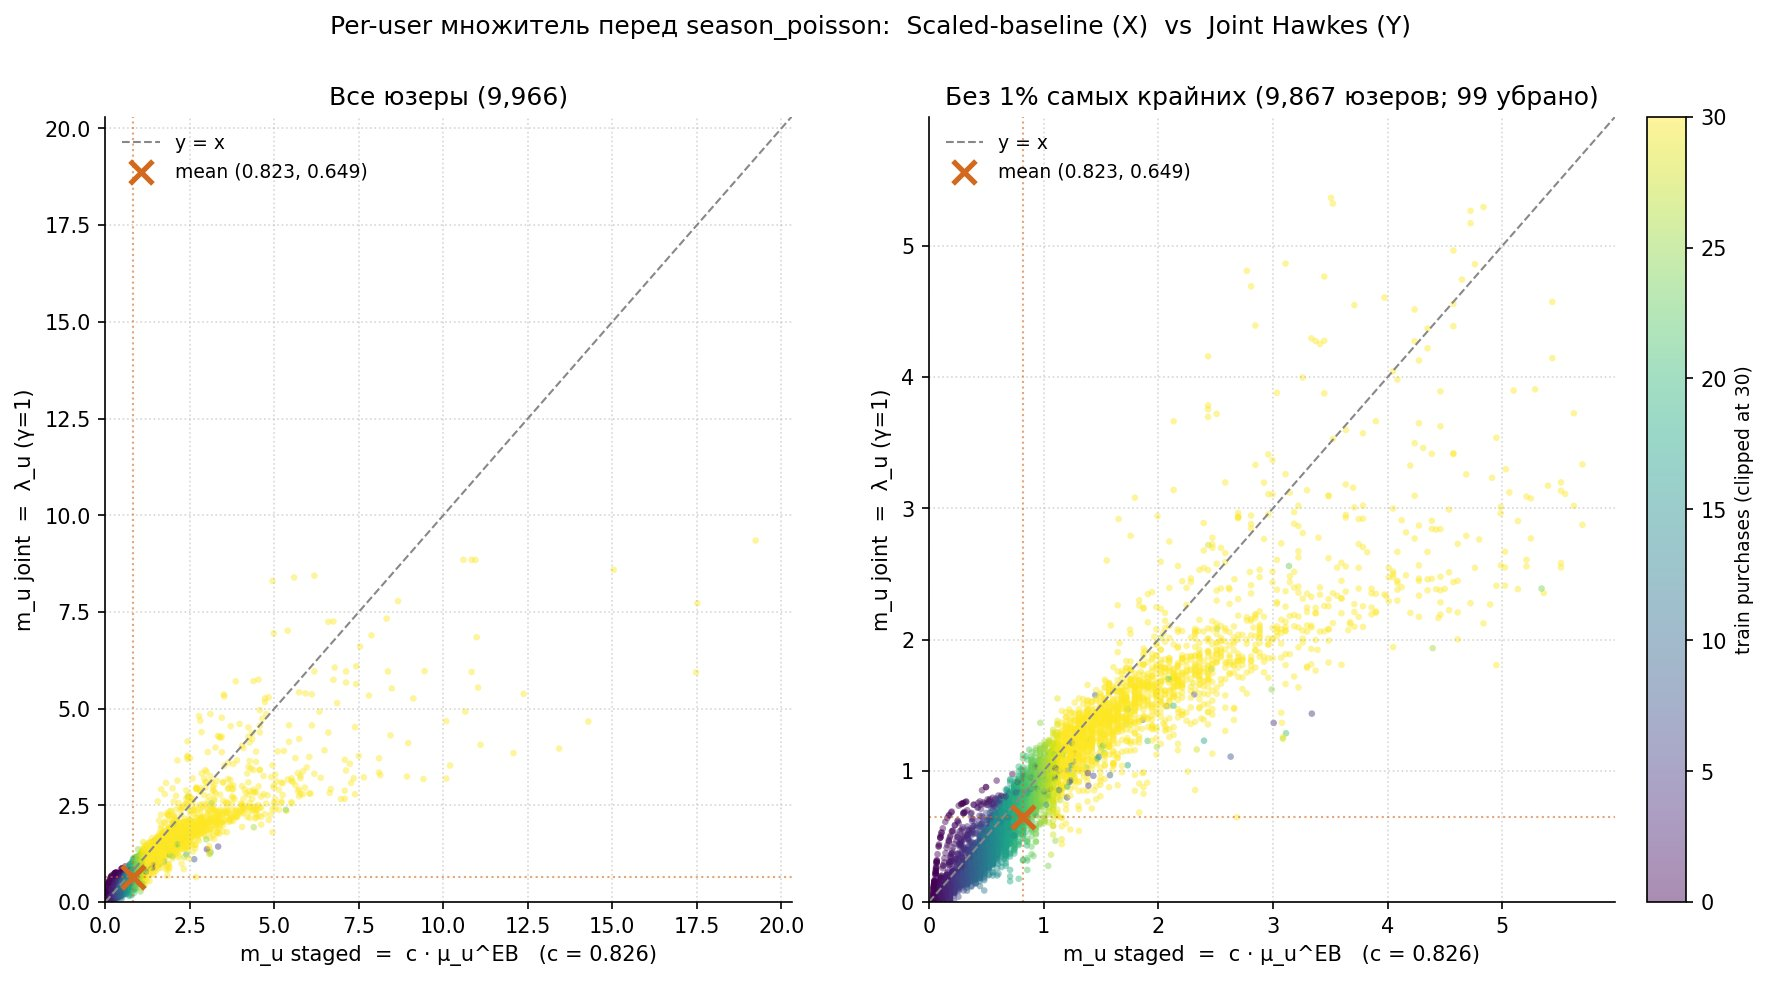
\includegraphics[width=0.85\textwidth]{images/fig13_multiplier_scatter.jpg}
\caption{Per-user m\_u: Scaled-baseline vs Joint Hawkes}
\end{figure}


Структурные эффекты:

\begin{itemize}
  \item \textbf{Средние значения} (красный крест): $m\_staged \approx  0.823$, $m\_joint \approx  0.649$. Joint в среднем занижает множитель сильнее, компенсируя это \textbf{примерно в 2 раза большим} $\|\alpha \|_2$ (\texttt{0.0324} vs \texttt{0.0161}).
  \item \textbf{Корреляция} \texttt{corr(m\_staged, m\_joint) = 0.85} - высокая, но не единица: модели договариваются о том, кто более активный, но конкретные значения отличаются.
  \item \textbf{Левый хвост} (юзеры с малым числом покупок) лежит \textbf{ниже диагонали}: для них Joint без явного EB-prior'а отпускает $\lambda _u$ в зону $\approx  0$, тогда как EB-shrunk база умножается на $c \approx  0.83$.
  \item \textbf{Активные пользователи} (правый хвост) тоже зачастую ниже диагонали: joint-фит снижает per-user multiplier, оставляя место большой Хоукс-надстройке.
\end{itemize}


Несмотря на эти разные декомпозиции, итоговый test NLL обоих моделей практически совпадает. Это и есть тот самый \textbf{$c-\alpha $ trade-off}: разные оценки $(m\_u, \alpha )$ дают почти одинаковую общую интенсивность. На уровне population-NLL модели неотличимы; на уровне внутренних параметров - существенно разные. Это наблюдение играет центральную роль в части III, где мы разворачиваем его в полноценный анализ identifiability через profile likelihood.

\clearpage
\section{Часть II. Поведение моделей на коротких train-окнах}

Все результаты Части I получены на \texttt{207}-дневном train. Возникает естественный вопрос: насколько эти выводы устойчивы к выбору train-окна? В индустриальных задачах часто доступны только короткие истории (\texttt{14..30} дней - например, в задачах быстрого онбординга новых сегментов или анализа A/B-эксперимента), и важно понять, какая параметризация Hawkes выживает на таких окнах.

\FloatBarrier
\subsection{Blockwise CV: 21-дневные блоки}

Первый эксперимент - blockwise cross-validation с непересекающимися 21-дневными блоками. Анализируемый период \texttt{2025-01-15..2025-09-30} бьётся на \texttt{13} блоков. В каждом блоке первые \texttt{14} дней используются как train, последние \texttt{7} - как test. Этот сплит несимметричный: ratio train/test = \texttt{2:1}, что соответствует характерной задаче коротких A/B-тестов, где данных для обучения мало. На каждом блоке независимо обучаются все шесть моделей лестницы плюс GBDT.


\begin{figure}[ht]
\centering
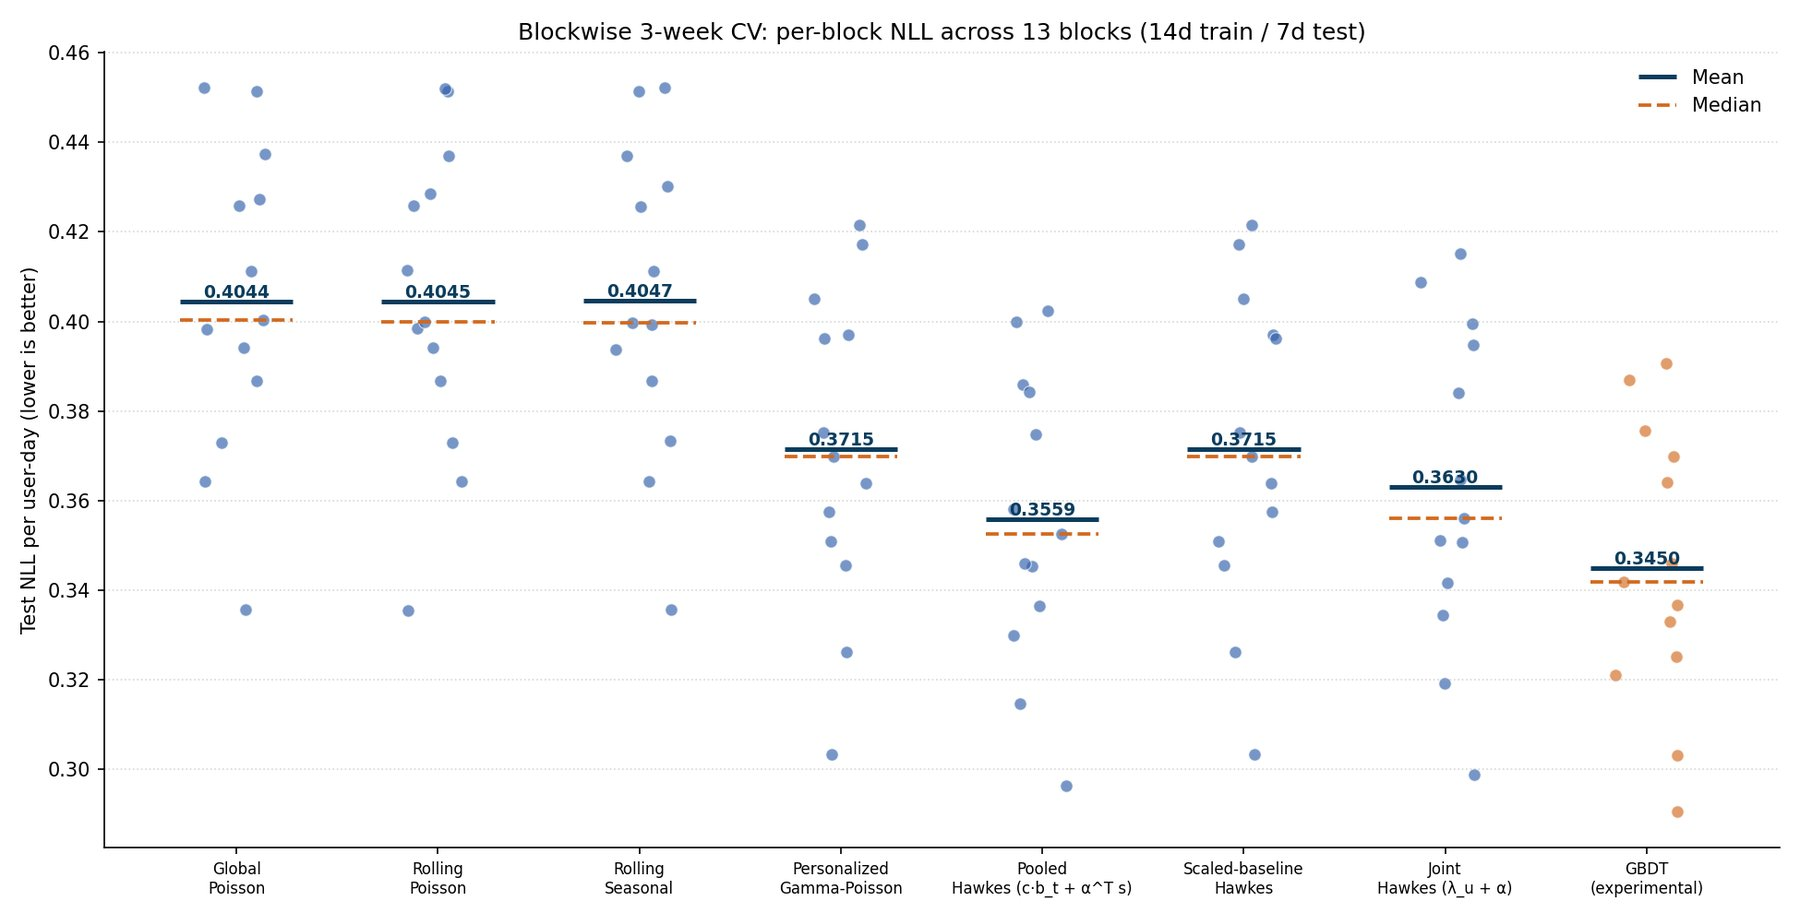
\includegraphics[width=0.85\textwidth]{images/fig14_cv_strip_plot.jpg}
\caption{Blockwise CV: per-block NLL}
\end{figure}


На коротких train (\texttt{14d}) картина меняется по сравнению с главным окном. Несколько ключевых наблюдений:

\begin{itemize}
  \item \textbf{Все «не персонализированные» бейзлайны} (Global, Rolling, Rolling Seasonal) дают практически одинаковый mean NLL \texttt{\textasciitilde{}0.404} и большой разброс по блокам (\texttt{0.34..0.45}). Они близки между собой, что и ожидаемо: рассчёт rolling-mean на 14 днях не сильно отличается от глобального среднего, а недельная сезонность на 14 днях оценивается шумно.
  \item \textbf{Personalized Gamma-Poisson} даёт mean NLL \texttt{\textasciitilde{}0.372} - заметное улучшение, но меньшее, чем на главном train (там было \texttt{\textasciitilde{}0.41}). Это связано с тем, что на 14 днях EB-prior сильнее доминирует - для большинства пользователей $Y\_u \approx  0..2$ покупок, и $\mu _u^{EB}$ лишь чуть отклоняется от prior'а.
  \item \textbf{Scaled-baseline Hawkes} даёт практически тот же mean NLL, что и Personalized GP - \texttt{\textasciitilde{}0.372}. Это указывает на вырождение, о котором речь дальше.
  \item \textbf{Joint Hawkes} даёт mean NLL \texttt{\textasciitilde{}0.363} - лучший среди вероятностных моделей, и заметно лучше Pers GP.
  \item \textbf{GBDT} остаётся лидером по абсолюту с mean NLL \texttt{\textasciitilde{}0.345}.
\end{itemize}


Дисперсия результатов по блокам велика для всех моделей. Это говорит о том, что на 14 днях существенную роль играет случайность выбора окна: блок с новогодним всплеском или без него даёт разные NLL даже у одной и той же модели.

\FloatBarrier
\subsection{Вырождение Scaled-baseline Hawkes}

Эффект вырождения Scaled-baseline Hawkes на 14d train особенно поучителен. Если посмотреть на обученные параметры на каждом блоке, видна следующая картина:

\begin{itemize}
  \item $\hat{c} \approx  1.00$ (зажат к prior'у \texttt{c = 1});
  \item $\|\alpha \|_2 \approx  0$ (все Хоукс-веса прижаты к нулю).
\end{itemize}


То есть модель \textbf{полностью теряет Хоукс-надстройку} и фактически сводится к Personalized GP. На уровне предсказательного качества это и подтверждается: их test NLL практически совпадают.

Причина - коллинеарность. На 14 днях \texttt{Y\_u} для большинства пользователей $\leq  2$, и EB-prior тянет $\mu _u^{EB}$ к среднему по когорте. Этот средний по когорте Hawkes-state \texttt{z\_\{u,j,t\}} пропорционален баесовскому уровню активности самого пользователя - то есть тому же сигналу, что $\mu _u^{EB} \cdot b\_t$. Линейный регрессор не может различить два почти коллинеарных сигнала и предпочитает оставить ровно один - бейзлайн-часть, поскольку именно её prior подталкивает \texttt{c → 1}.

Это и есть проявление известного из multivariate Хоукс-литературы эффекта [4]: на малом числе наблюдений диагональные компоненты влияния не идентифицируются и поглощаются фоновой интенсивностью. В нашем случае это происходит не на cross-channel диагонали (мы ещё не в cross-channel постановке), а на «временной» диагонали - между $\mu _u$ и self-history \texttt{z\_\{u, to\_ord, t\}} для целевого канала.

Вырождение мотивирует переход к другой форме обучения, которая бы не позволяла Хоукс-надстройке схлопнуться к нулю.

\FloatBarrier
\subsection{Joint Hawkes на коротких окнах}

Joint Hawkes (определение и обучение разобраны в Части I) построен так, что вместо двухступенчатого EB-prior'а на $\mu _u$ использует явную L2-регуляризацию per-user множителей $(\lambda _u - 1)^2$ напрямую при совместной оптимизации с $\alpha $. Это отличие, малозаметное на полном train (test NLL практически одинаковый со Scaled-baseline), оказывается решающим на коротких окнах.

Активный L2-prior удерживает $\lambda _u$ в окрестности единицы: оптимизатор не может «зажать» все $\lambda _u$ в ноль и переложить весь сигнал на Хоукс-часть (или наоборот). На \texttt{14d}-train Joint Hawkes \textbf{не вырождается}: $\|\alpha \|_2 \approx  0.04..0.05$ на всех \texttt{n} от 15 до 200 дней. То есть Хоукс-надстройка остаётся ненулевой и информативной даже там, где у Scaled-baseline она схлопывается до нуля.

По умолчанию используем $\lambda _{\ell_2} = 1$ как «активный prior». Чувствительность результата к этой константе подробно разбираем в Части III; здесь она фиксирована.

\FloatBarrier
\subsection{Train-length scan и crossover'ы}

Систематический анализ - sweep по длине train-окна $n \in  \{15, 21, 27, 36, 48, 63, 84, 114, 153, 198\}$ дней. На каждом значении \texttt{n} берётся \texttt{m} случайных интервалов из анализируемого периода (с фиксированным seed), и для каждого интервала строится разбиение \texttt{2n/3} train + \texttt{n/3} test. На каждом запуске обучаются все семь моделей. Это позволяет получить distribution test NLL для каждой пары \texttt{(модель, n)} и оценить как mean, так и дисперсию.

Сводный график mean test NLL по моделям от \texttt{n} - рис. 13.


\begin{figure}[ht]
\centering
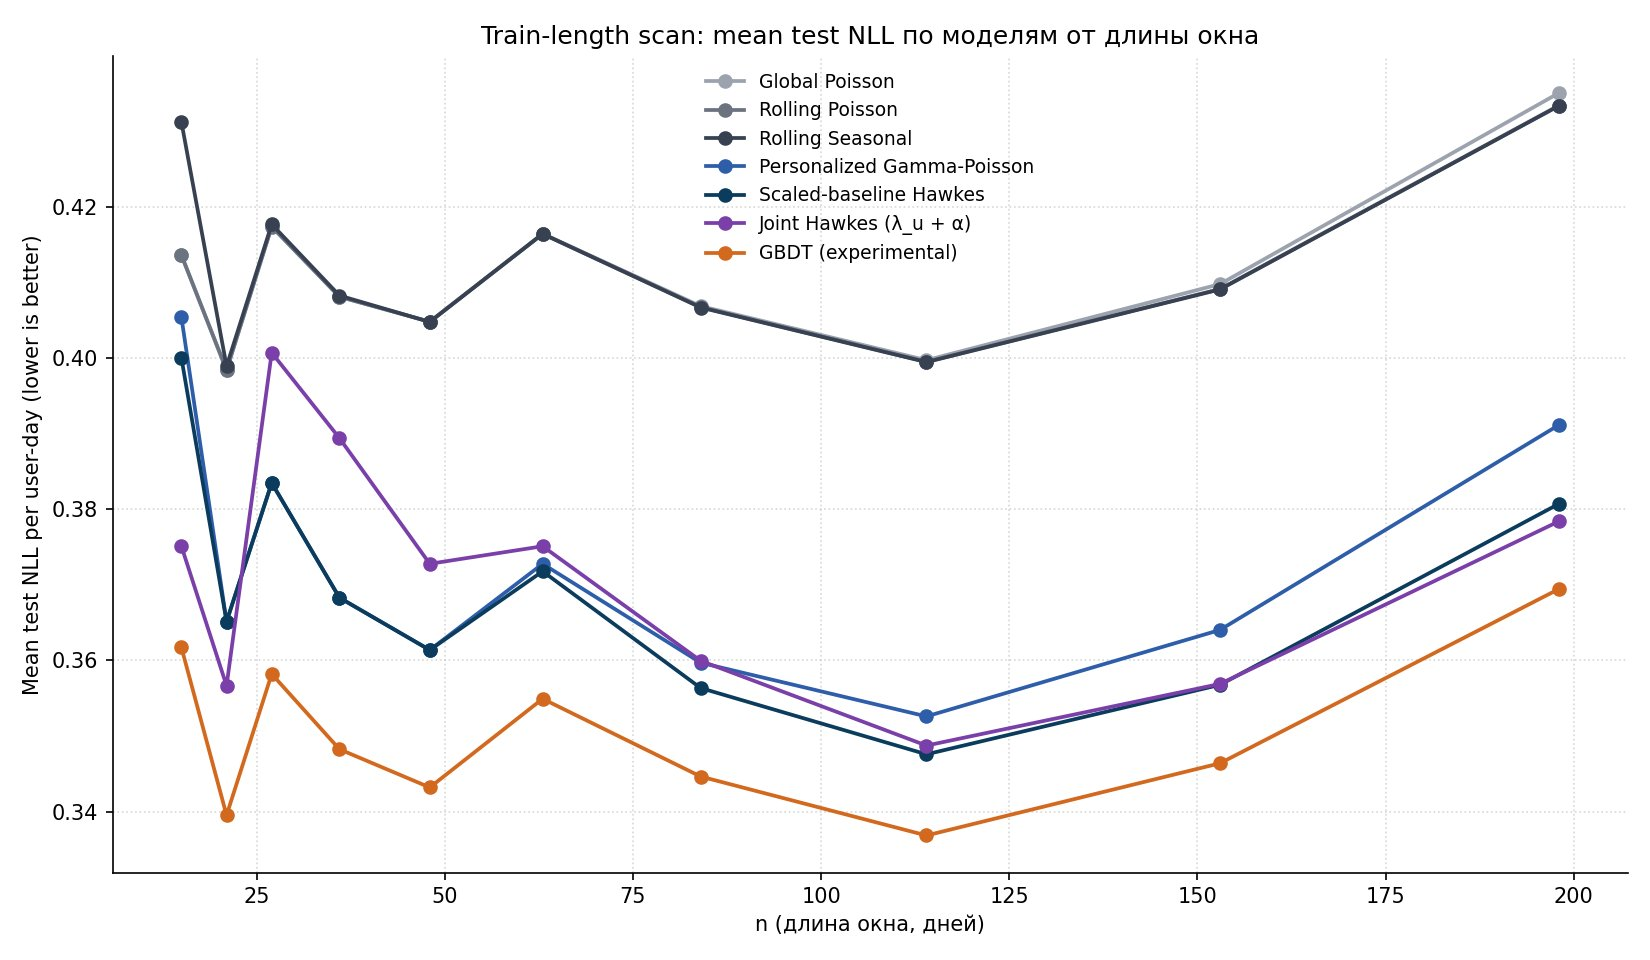
\includegraphics[width=0.85\textwidth]{images/fig15_mean_nll_vs_n_no_pooled.jpg}
\caption{Mean NLL по моделям от длины окна}
\end{figure}


Виден чёткий crossover между моделями:

\begin{itemize}
  \item На $n \leq  21$ Joint Hawkes слегка опережает Scaled-baseline и Personalized GP (зазор \texttt{\textasciitilde{}0.02..0.05} в NLL). Это та самая зона, где Scaled вырождается, а Joint удерживает Хоукс-сигнал.
  \item На $n \in  [27, 60]$ все три вероятностные модели сходятся в почти одну точку. Это переходная зона: Scaled постепенно начинает «находить» Хоукс-надстройку, но ещё не дотягивает до Joint.
  \item На $n \geq  100$ Scaled-baseline Hawkes и Joint Hawkes становятся почти одинаковыми и оба обходят Personalized GP на \texttt{\textasciitilde{}0.02} в NLL. Это зона «полной информации»: данных достаточно, чтобы любая из двух Хоукс-параметризаций сошлась к одному и тому же оптимуму.
\end{itemize}


GBDT остаётся лучшим в абсолюте на всех \texttt{n}, но \textbf{разрыв уменьшается с ростом \texttt{n}} - на длинных train probabilistic-модели догоняют бустинг. На \texttt{n = 198} день разрыв Joint Hawkes vs GBDT составляет \texttt{\textasciitilde{}0.009} в NLL против \texttt{\textasciitilde{}0.014} на \texttt{n = 15}.

Поведение нормы Хоукс-коэффициентов и среднего per-user multiplier'а от \texttt{n} - рис. 14 и 15.


\begin{figure}[H]
\centering
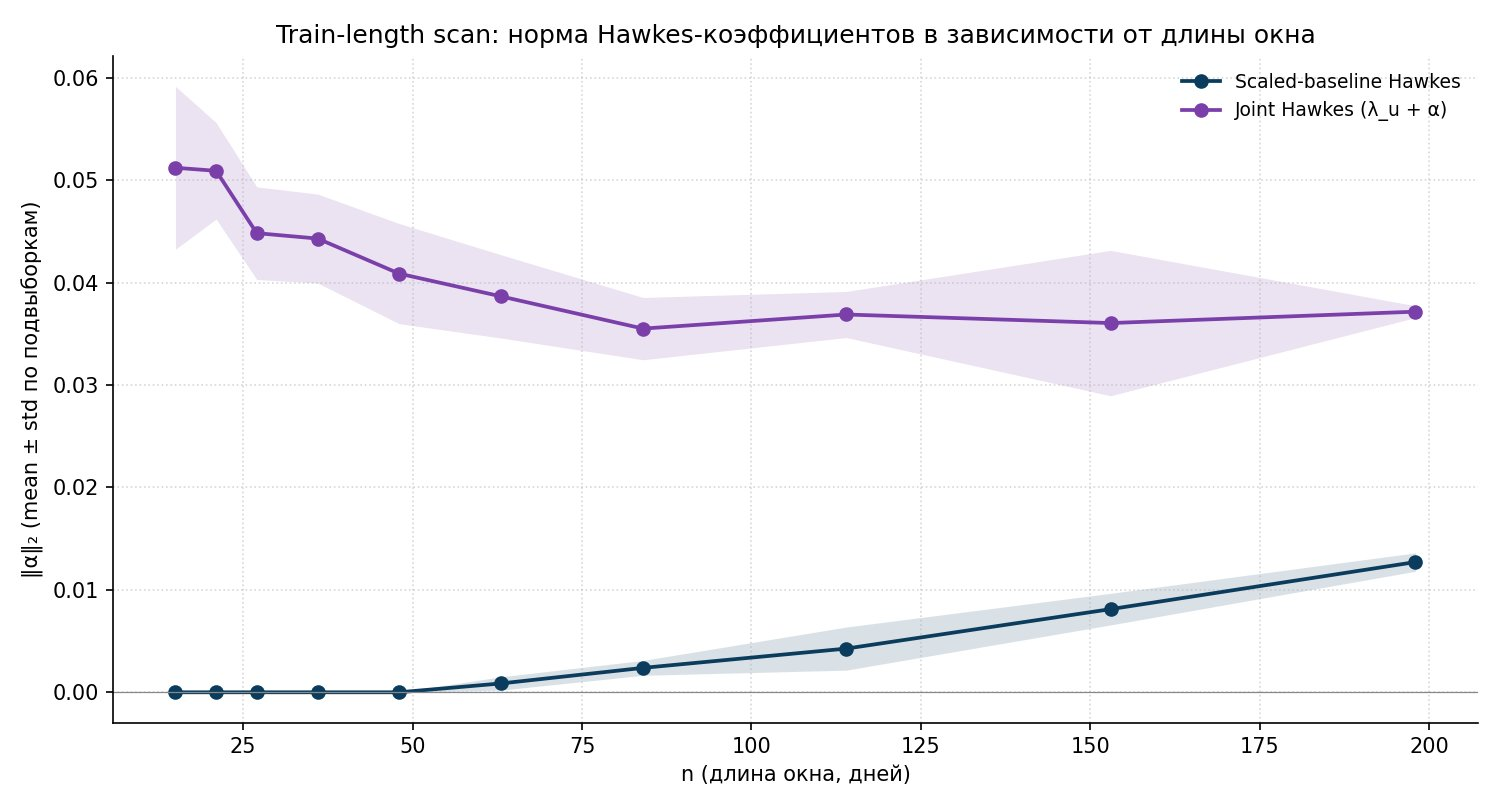
\includegraphics[width=0.85\textwidth]{images/fig16_alpha_norm_vs_n_no_pooled.jpg}
\caption{Норма $\|\alpha\|_2$ по моделям от длины окна}
\end{figure}


\begin{figure}[H]
\centering
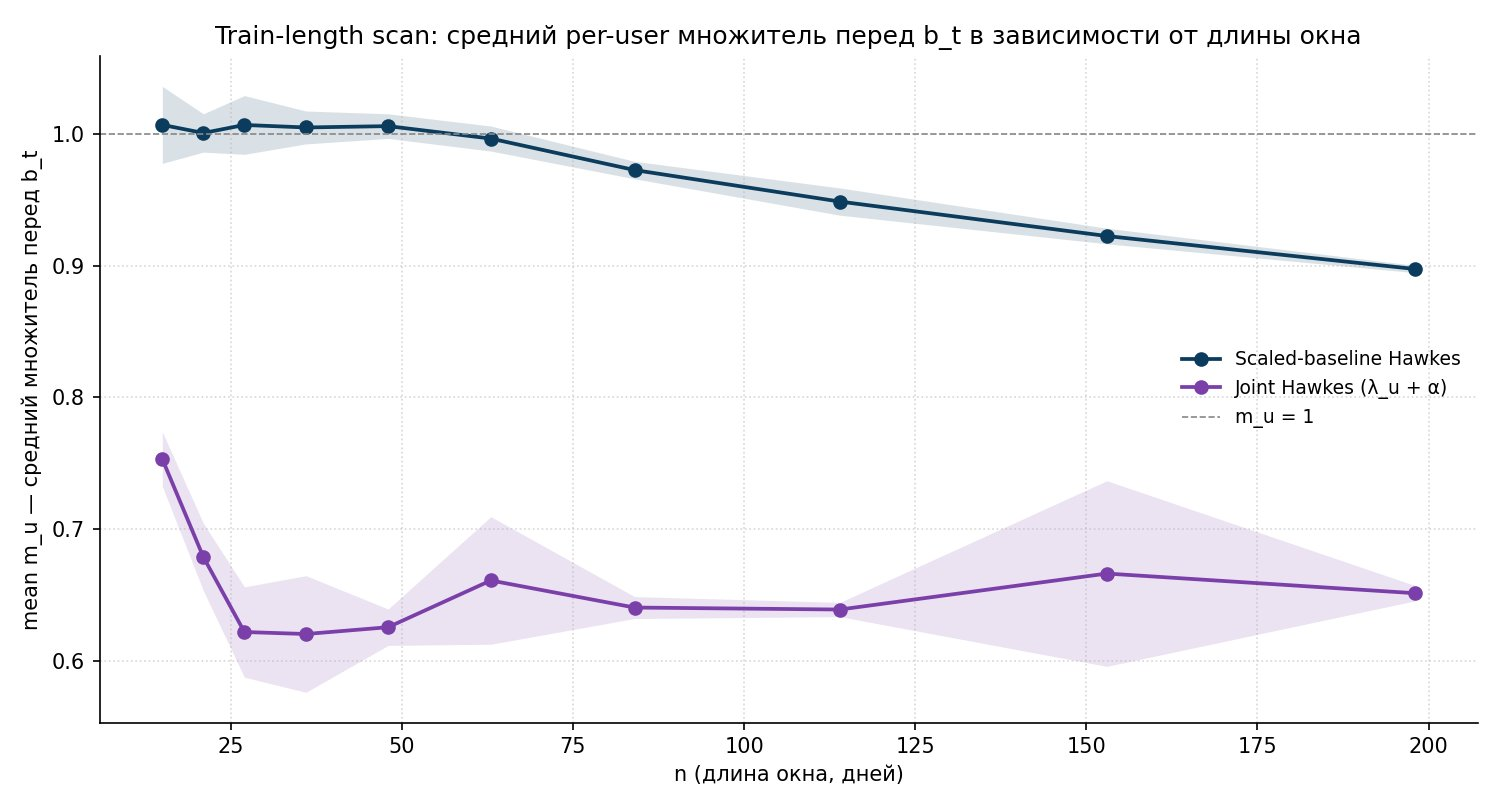
\includegraphics[width=0.85\textwidth]{images/fig17_m_u_mean_vs_n_no_pooled.jpg}
\caption{Средний per-user multiplier от длины окна}
\end{figure}

Здесь хорошо видно вырождение: для Scaled-baseline $\|\alpha \| = 0$ на всех $n \leq  50$ (плоское ноль), и только с $n \approx  80$ норма начинает расти. На \texttt{n = 198} норма достигает \texttt{\textasciitilde{}0.012}, что близко к значению \texttt{\textasciitilde{}0.016}, полученному на полном \texttt{207d}-train. У Joint Hawkes $\|\alpha \|$ стабилен (\texttt{\textasciitilde{}0.04..0.05}) с самого \texttt{n = 15}, медленно убывая к \texttt{\textasciitilde{}0.037} на больших \texttt{n}. Mean per-user multiplier $\lambda _u$ у Joint Hawkes держится \texttt{\textasciitilde{}0.65..0.75} независимо от \texttt{n}, что согласуется с активной L2-регуляризацией к единице.

Главный вывод этой части: \textbf{нет универсально лучшей Хоукс-параметризации}, выбор зависит от длины train. На коротких окнах работает Joint Hawkes с активной регуляризацией, на длинных оба Хоукс-варианта эквивалентны. Для индустриальной практики это означает, что в системе с переменной длиной обучающего окна (например, в continuous learning pipeline) имеет смысл использовать Joint Hawkes как default-вариант: он не теряет качества на длинных train и не вырождается на коротких.

\clearpage
\section{Часть III. Структура cross-channel Хоукс-матрицы}

В первой части мы рассматривали один target - \texttt{to\_ord} - и вектор $\alpha $ по нескольким source-каналам. В этой части переходим к \textbf{cross-channel постановке}: на каждый из трёх каналов воронки (\texttt{searches}, \texttt{to\_cart}, \texttt{to\_ord}) подгоняется собственная Хоукс-модель, у которой источниками возбуждения служат \textbf{все три канала} (включая сам себя). Получается интерпретируемая матрица $\alpha  \in  \mathbb{R}^{3\times 3}$ пар-канальных взаимодействий - диагональ описывает self-excitation каждого канала, off-diagonal - cross-channel влияние.

\FloatBarrier
\subsection{Cross-channel постановка и верификация}

Для каждой пары \texttt{(target, source)} Hawkes-state строится с тем же полураспадом 1 день, и оптимизация выполняется отдельно по каждому target'у. Модель для одного target'а:

\[
\lambda^{(k)}_{u,t} \;=\; c_k \cdot \mu_u^{\mathrm{EB},k} \cdot b_t^{(k)} \;+\; \sum_{j=1}^{3} \alpha_{kj} \cdot z_{u,j,t},
\]

где индекс \texttt{k} пробегает 3 канала. На главном \texttt{207d}-train у Scaled-baseline Hawkes получается матрица:


\begin{table}[ht]
\centering
\small
\begin{tabular}{lrrr}
\toprule
target ↓ \textbackslash{} source $\to$ & \texttt{searches} & \texttt{to\_cart} & \texttt{to\_ord} \\
\midrule
\texttt{searches} & \texttt{0.1269} & \texttt{0.0240} & \texttt{0} \\
\texttt{to\_cart} & \texttt{0.0103} & \texttt{0.0713} & \texttt{0} \\
\texttt{to\_ord} & \texttt{0.0030} & \texttt{0.0046} & \texttt{0.0194} \\
\bottomrule
\end{tabular}
\end{table}


Визуально (рис. 16):


\begin{figure}[ht]
\centering
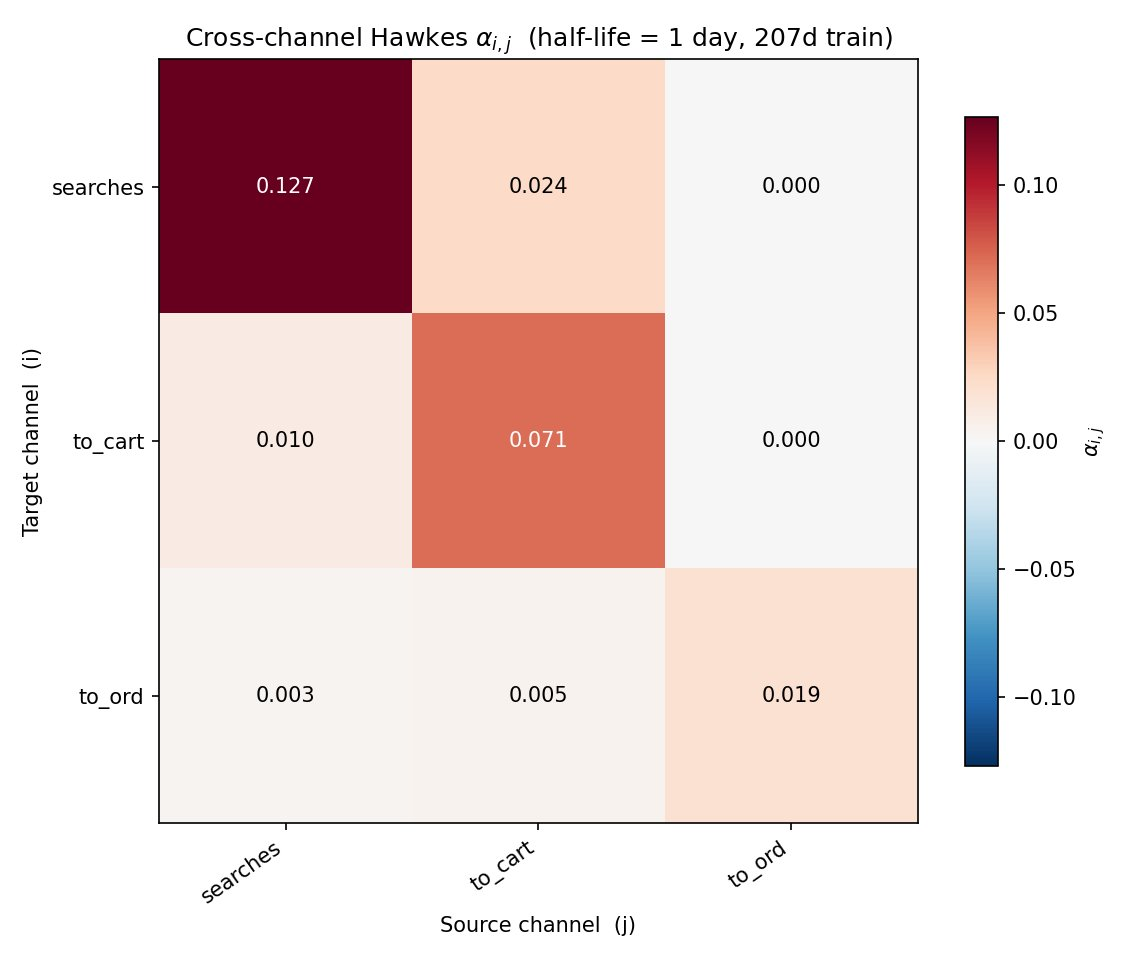
\includegraphics[width=0.7\textwidth]{images/fig18_alpha_heatmap.jpg}
\caption{Cross-channel α-матрица на главном train (Scaled-baseline)}
\end{figure}


Структура воронки видна сразу:

\begin{itemize}
  \item \textbf{Верхне-треугольная часть колонки \texttt{to\_ord} идентически нулевая}: после покупки нет краткосрочного Хоукс-сигнала на поиск или корзину. Это структурный нуль, который мы интерпретируем как отсутствие «обратного» возбуждения в воронке: купив товар, пользователь не идёт сразу искать ещё.
  \item \textbf{Off-diagonal funnel-связи \texttt{searches → cart → order}} различимы и положительны: например, $\alpha [to\_cart \leftarrow  searches] = 0.010$ и $\alpha [to\_ord \leftarrow  to\_cart] = 0.0046$. Это согласуется с физической воронкой: поиск повышает интенсивность добавления в корзину, корзина повышает интенсивность покупки.
  \item \textbf{Self-$\alpha$ $\alpha [to\_ord \leftarrow  to\_ord] = 0.019$} ненулевой, но небольшой. Этот коэффициент окажется главным героем последующих разделов: он плохо идентифицируем на коротких train и сильно зависит от регуляризации.
\end{itemize}


Прежде чем интерпретировать матрицу подробнее, стоит убедиться, что Хоукс-надстройка вообще полезна для каждого из трёх каналов (для \texttt{to\_ord} это уже показано в части I, но \texttt{searches} и \texttt{to\_cart} - новые target'ы). Сравнение test NLL Personalized GP без Hawkes vs Scaled Hawkes на трёх каналах - рис. 17.


\begin{figure}[H]
\centering
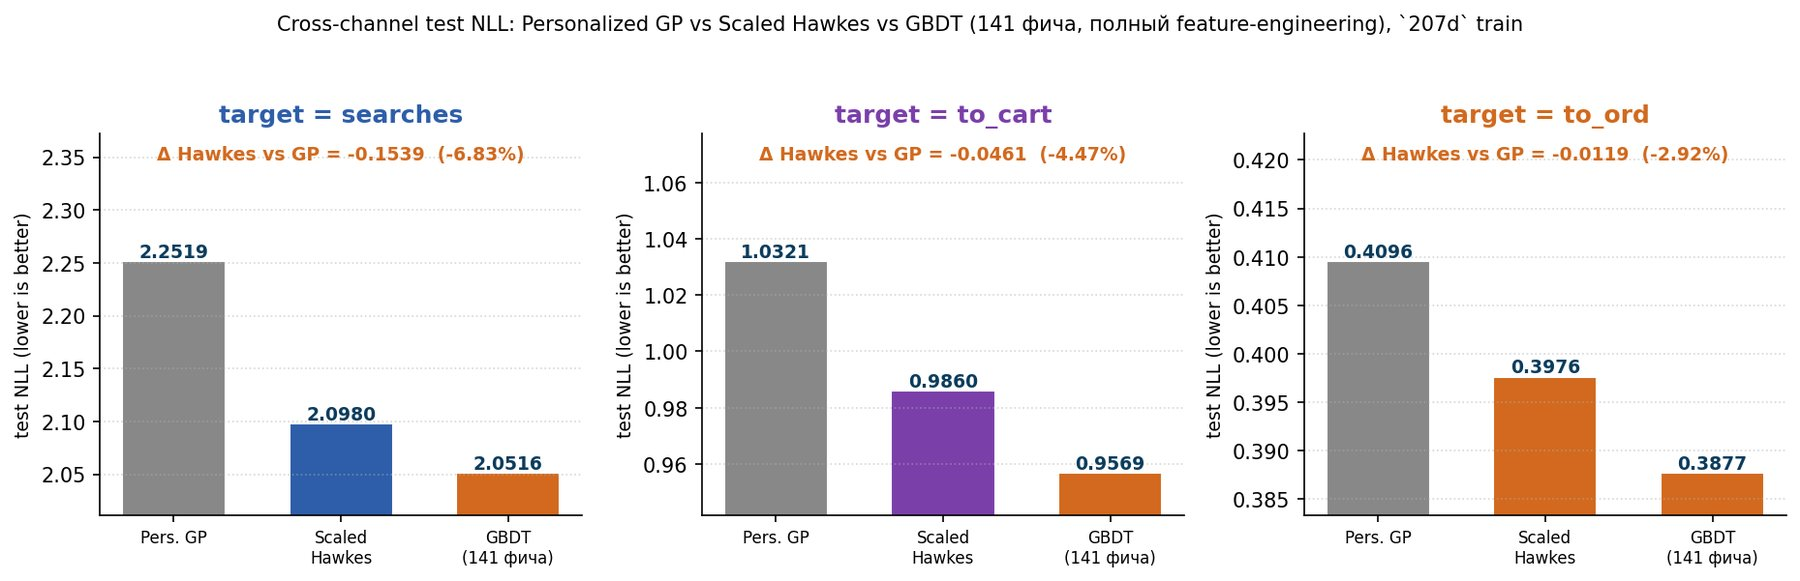
\includegraphics[width=0.7\textwidth]{images/fig19_baseline_vs_hawkes_nll.jpg}
\caption{Per-channel верификация: Pers GP vs Scaled Hawkes vs GBDT}
\end{figure}


Хоукс-надстройка улучшает бейзлайн на всех трёх каналах: на \texttt{searches} - \texttt{-6.83\%} от бейзлайна NLL, на \texttt{to\_cart} - \texttt{-4.47\%}, на \texttt{to\_ord} - \texttt{-2.92\%}. Относительное улучшение монотонно убывает по плотности target'а, что согласуется с интуицией: на разреженном \texttt{to\_ord} Хоукс-сигнал относительно baseline слабее.

На том же рисунке показан третий bar - GBDT на полном feature-engineering'е (141 фича) для каждого из 3 каналов. Бустинг обгоняет Hawkes на всех трёх каналах ещё на \texttt{2.21..2.95\%} от бейзлайна, давая верхнюю планку. При этом Hawkes закрывает \textbf{\texttt{54..77\%} суммарного gap'а} от Pers GP до GBDT - большую часть выжимаемого сигнала, ценой более простой структуры и интерпретируемости. Это та же картина trade-off, что и в части I, теперь воспроизведённая отдельно на каждом канале.

\FloatBarrier
\subsection{Чувствительность к регуляризации}

Структурно матрица $\alpha $ показывает интерпретируемые свойства, но bootstrap-анализ по 10 случайным \texttt{100d}-окнам обнаруживает важную нестабильность. Mean ± std по окнам для Scaled-baseline:


\begin{table}[ht]
\centering
\small
\begin{tabular}{lrrr}
\toprule
ячейка & mean $\alpha $ & std & CV \\
\midrule
\texttt{searches ← searches} & \texttt{0.0798} & \texttt{0.0058} & \texttt{7.2\%} \\
\texttt{searches ← to\_cart} & \texttt{0.0168} & \texttt{0.0026} & \texttt{15.5\%} \\
\texttt{to\_cart ← searches} & \texttt{0.0060} & \texttt{0.0009} & \texttt{15.6\%} \\
\texttt{to\_cart ← to\_cart} & \texttt{0.0347} & \texttt{0.0034} & \texttt{9.7\%} \\
\texttt{to\_ord ← searches} & \texttt{0.0011} & \texttt{0.0005} & \texttt{47.4\%} \\
\texttt{to\_ord ← to\_cart} & \texttt{0.0025} & \texttt{0.0009} & \texttt{36.2\%} \\
\textbf{\texttt{to\_ord ← to\_ord}} & \textbf{\texttt{0.0016}} & \textbf{\texttt{0.0024}} & \textbf{\texttt{148.3\%}} \\
\bottomrule
\end{tabular}
\end{table}


Off-diagonal funnel-связи стабильны ($CV \leq  16\%$ для частых пар, до \texttt{47\%} для редкого \texttt{to\_ord ← searches}), но \textbf{$\alpha [to\_ord \leftarrow  to\_ord]$ коллапсирует}: median $\approx$ \texttt{0}, в части окон значение зажимается к нулю. Это - та же история, что и в части II (вырождение Scaled-baseline на коротких train), теперь видимая в cross-channel постановке: EB-prior зажимает per-user multiplier к нулю для редко-активных пользователей, и у оптимизатора нет signal для self-$\alpha$ редкого target'а.

Переход к Joint Hawkes с активной регуляризацией решает эту проблему. На том же bootstrap'е Joint Hawkes с $\lambda _{\ell_2} = 1$ удерживает $\alpha [to\_ord \leftarrow  to\_ord] = 0.038$ с CV \texttt{14.7\%}. Если же отключить регуляризацию ($\lambda _{\ell_2} = 0$), self-$\alpha$ снова коллапсирует до \texttt{0.0002} с CV \texttt{316\%}. Сравнение трёх режимов - рис. 18.


\begin{figure}[ht]
\centering
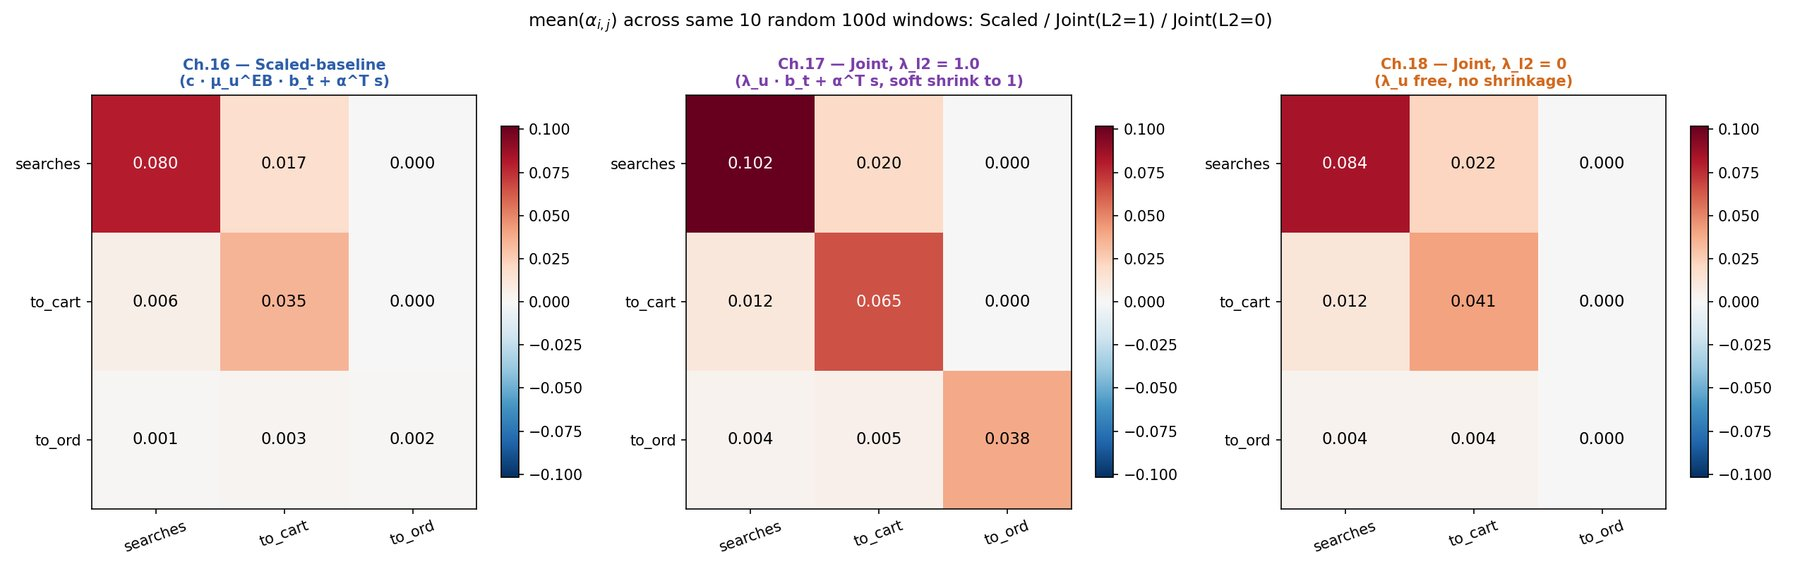
\includegraphics[width=0.85\textwidth]{images/fig20_alpha_compare_three_way.jpg}
\caption{Сравнение трёх режимов: Scaled vs Joint(λ\_l2=1) vs Joint(λ\_l2=0)}
\end{figure}


Из этого следует важный вывод: \textbf{коэффициенты cross-channel матрицы сильно зависят от регуляризации}, причём особенно сильно - диагональные. Off-diagonal элементы стабильны во всех трёх режимах. При этом регуляризация может быть \textbf{структурной} (как между Personalized GP с EB-регуляризацией и Joint Hawkes с L2-prior'ом к единице), либо \textbf{численной} (как внутри Joint Hawkes - $\lambda _{\ell_2} = 1$ vs $\lambda _{\ell_2} = 0$). Оба типа эквивалентны по своему влиянию на диагональ.

Чтобы понять, как именно регуляризация перераспределяет внутреннюю структуру модели, проведён sweep по $\lambda _{\ell_2} \in  \{0, 0.01, 0.05, 0.1, 0.3, 0.5, 1, 2, 5\}$ на главном \texttt{207d}-train для каждого из 3 target'ов. Поведение разложения интенсивности на бейзлайн-часть $\lambda _u \cdot  b\_t$ и Хоукс-часть $\alpha ^{\top} z$ показано на рис. 19.


\begin{figure}[ht]
\centering
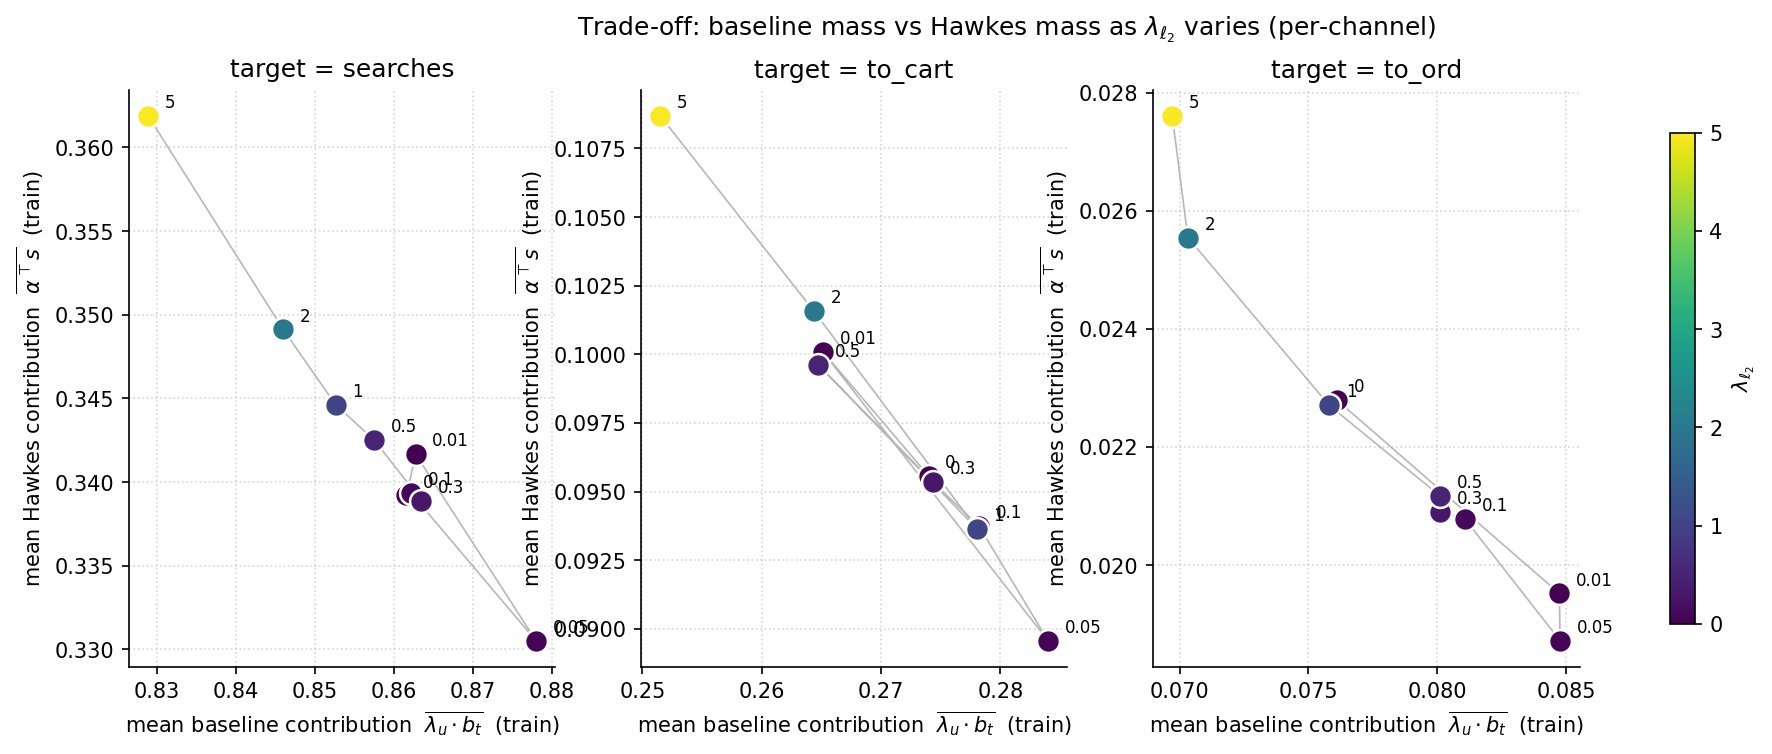
\includegraphics[width=0.85\textwidth]{images/fig21_tradeoff_cloud.jpg}
\caption{Trade-off: масса baseline vs Hawkes от λ\_l2}
\end{figure}


С ростом $\lambda _{\ell_2}$ оптимизатор зажимает $\lambda _u$ к \texttt{1}, и часть общей массы интенсивности \textbf{перетекает из бейзлайн-части $\lambda _u \cdot  b\_t$ в Хоукс-надстройку $\alpha ^{\top} z$} - на всех 3 каналах. Сильнее всего на редком \texttt{to\_ord}: при $\lambda _{\ell_2} = 0$ базовая часть составляет \texttt{0.085} в NLL, при $\lambda _{\ell_2} = 5$ - \texttt{0.069}, а Хоукс-часть растёт с \texttt{0.019} до \texttt{0.028}. То есть $\alpha $ явно выступает \textbf{компенсаторной переменной} относительно зажатия $\lambda _u$.

При этом test NLL \textbf{почти не меняется} по всей сетке $\lambda _{\ell_2}$ (рис. 20):


\begin{figure}[ht]
\centering
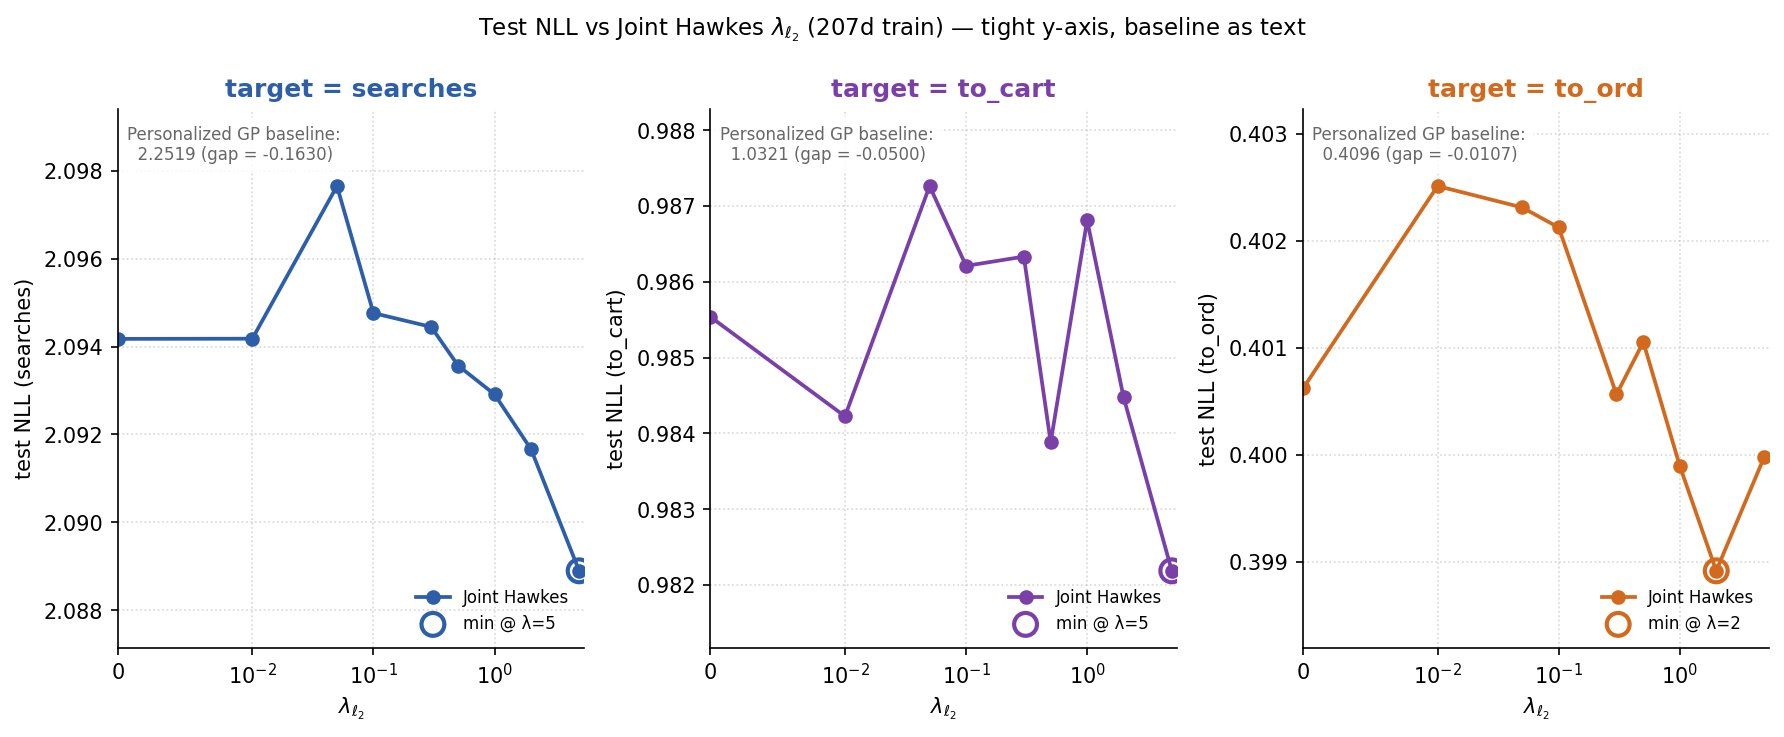
\includegraphics[width=0.85\textwidth]{images/fig22_test_nll_vs_lambda.jpg}
\caption{Test NLL от λ\_l2}
\end{figure}


Размах test NLL: \texttt{searches} $\approx$ \texttt{0.009}, \texttt{to\_cart} $\approx$ \texttt{0.005}, \texttt{to\_ord} $\approx$ \texttt{0.004}. Это значит, что \textbf{разные $\lambda _{\ell_2}$ дают существенно разные разложения $(\lambda _u, \alpha )$, но почти одинаковое predicted intensity на test}. Модель сверх-параметризована на уровне внутренних параметров, при том что её предсказательное качество устойчиво.

Разрешение $\alpha $ по $\lambda _{\ell_2}$ - рис. 21.


\begin{figure}[ht]
\centering
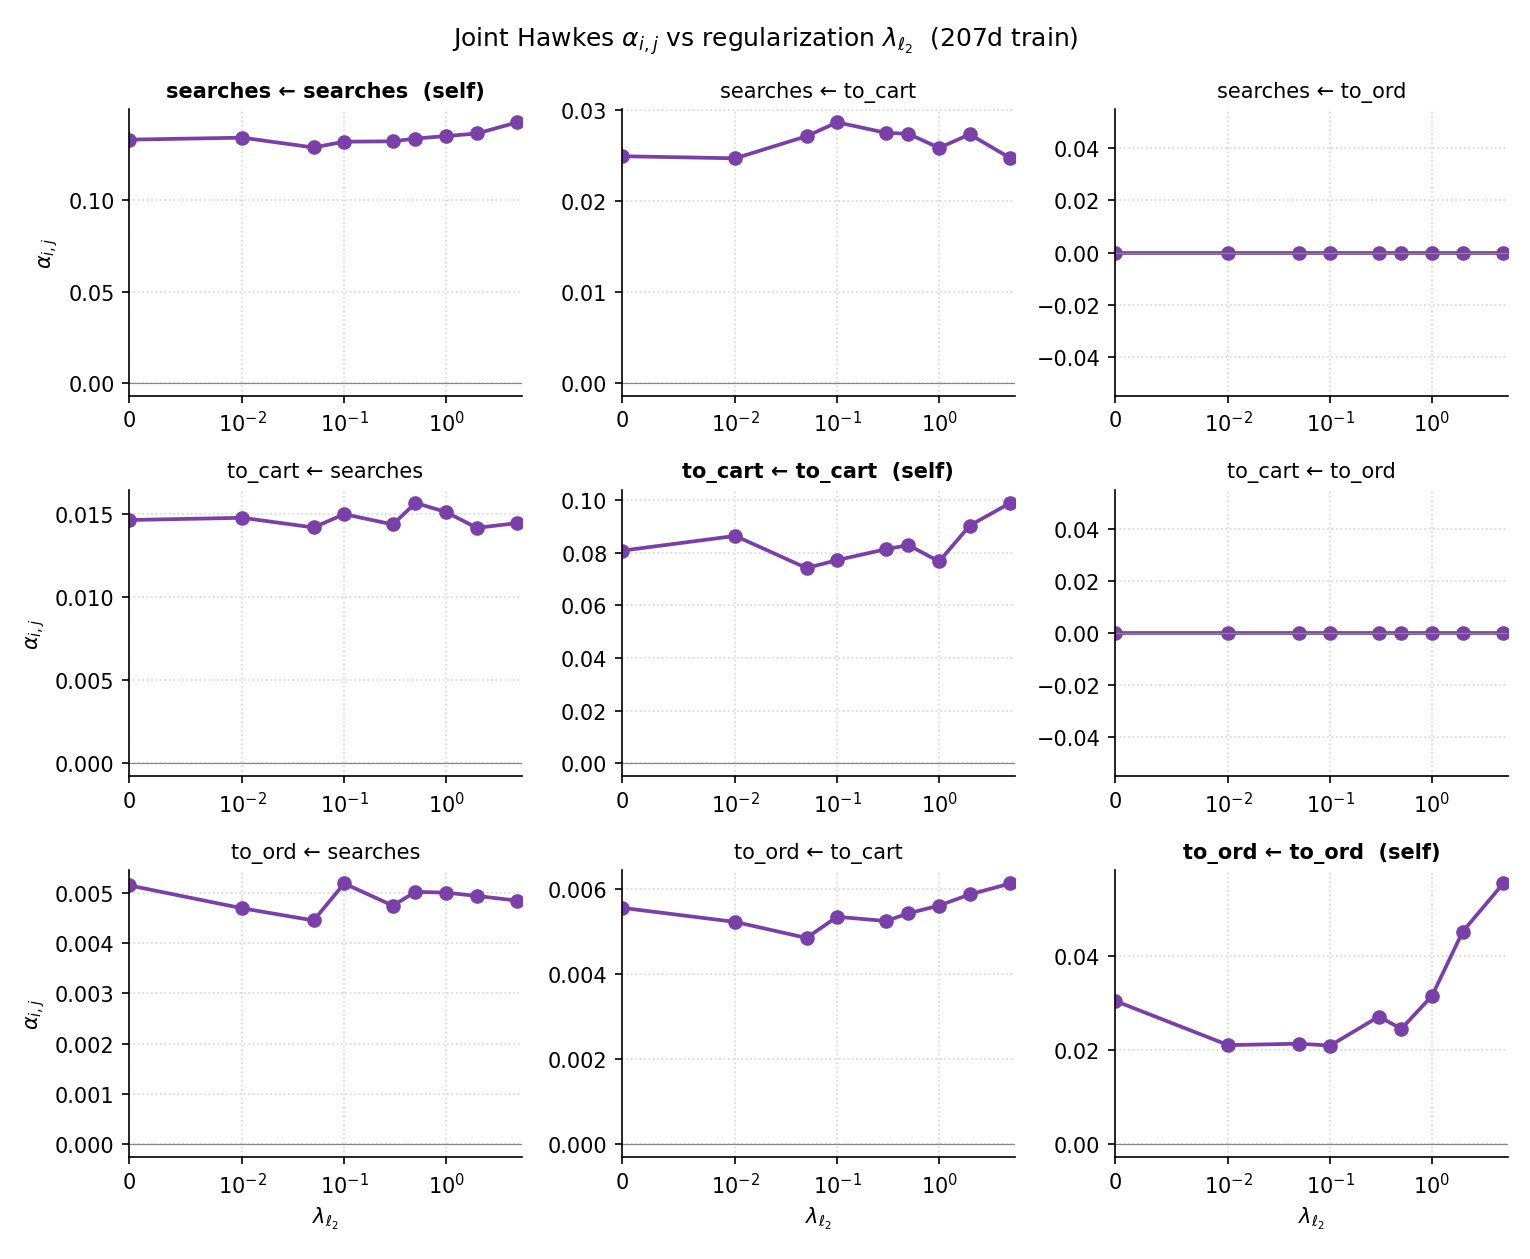
\includegraphics[width=0.85\textwidth]{images/fig23_alpha_vs_lambda_grid.jpg}
\caption{Зависимость α от λ\_l2 - 3×3 сетка}
\end{figure}


Картина характеристическая:

\begin{itemize}
  \item Колонка \texttt{to\_ord} - идентический ноль на всём grid'е (структурный результат).
  \item Off-diagonal funnel-связи устойчивы (\texttt{±2..10\%} по всему диапазону).
  \item $\alpha [searches \leftarrow  searches]$ устойчив (\texttt{±4\%}): \texttt{0.133 → 0.143}.
  \item $\alpha [to\_cart \leftarrow  to\_cart]$ умеренно меняется (\texttt{±13\%}): \texttt{0.081 → 0.099}.
  \item \textbf{$\alpha [to\_ord \leftarrow  to\_ord]$ сильно зависит от prior'а (\texttt{+82\%})}: \texttt{0.030 → 0.055}.
\end{itemize}


Внутренняя структура модели поэтому несимметрична: внедиагональные коэффициенты - это «коэффициенты данных», диагональные - особенно $\alpha [to\_ord \leftarrow  to\_ord]$ - это «коэффициенты prior'а». Этот вывод формализуется в следующем разделе через profile likelihood.

\FloatBarrier
\subsection{Profile likelihood и асимметрия диагонали/внедиагональных}

Чтобы напрямую измерить идентифицируемость каждого коэффициента, мы используем \textbf{profile likelihood}. Для каждой пары \texttt{(target, source)}:

\begin{enumerate}
  \item Сначала проводим cold-fit unfixed Joint Hawkes - получаем anchor $(\hat{\lambda}_u, \hat{\alpha})$.
  \item Строим pin-grid из 11 точек вокруг unfixed значения: $linspace(0, max(0.10, 2 \cdot  \hat{\alpha}_{\text{source}}), 11)$.
  \item Фиксируем $\alpha [target \leftarrow  source]$ на каждой точке grid'а; ре-оптимизируем $\lambda _u$ и оставшиеся 2 коэффициента $\alpha [target, \cdot ]$.
  \item Считаем train NLL и test NLL для каждой из 11 точек.
\end{enumerate}


Для устойчивости оптимизации используется warm-start sequential sweep: начинаем с точки grid'а, ближайшей к anchor'у, и постепенно расширяемся вверх и вниз; затем два polish-pass'а с re-anchor на текущий best. Это исключает дискретные скачки в profile NLL из-за плохой инициализации.

Полная картина 3$\times$3 для train NLL приведена на рис. 22, для test NLL - на рис. 23.


\begin{figure}[ht]
\centering
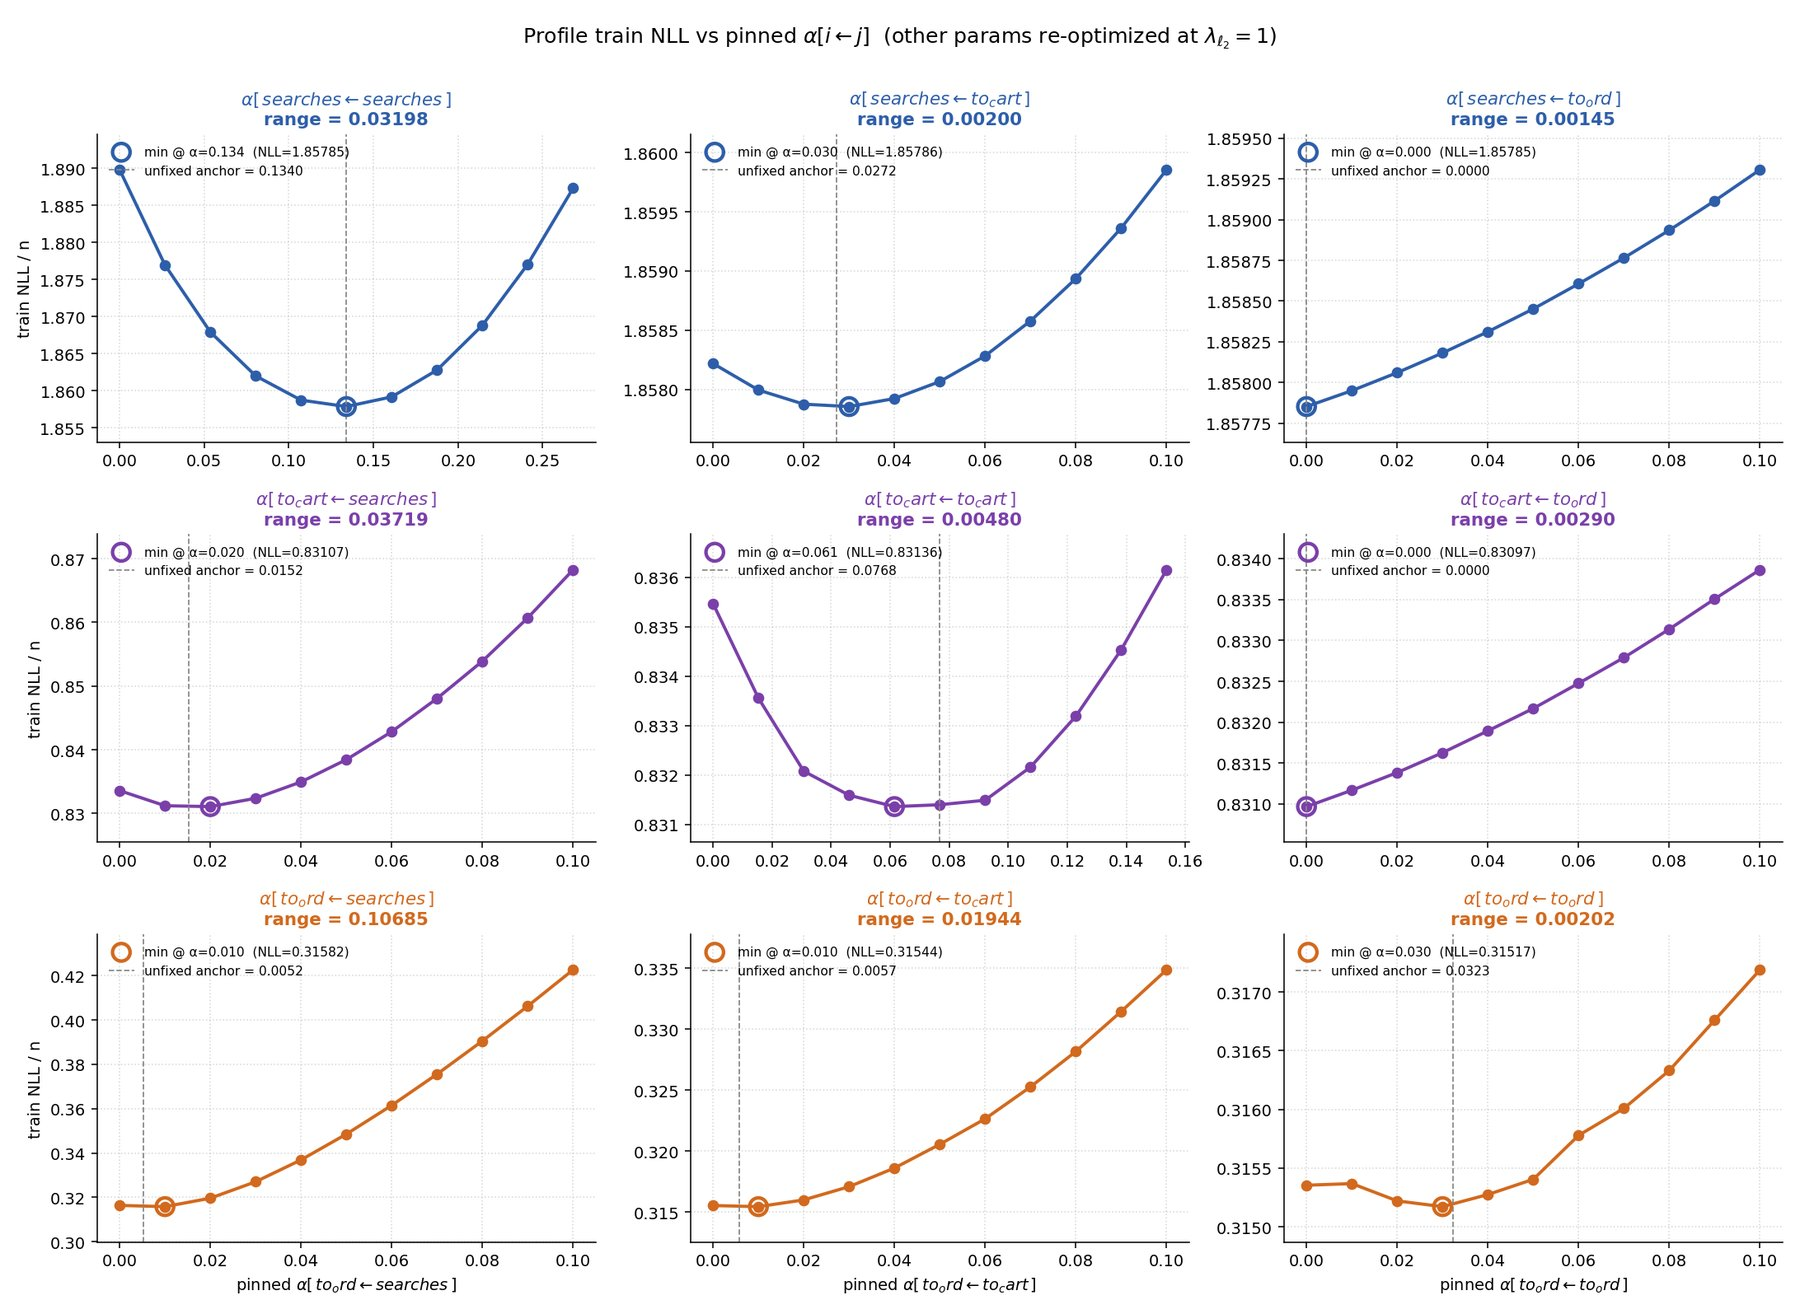
\includegraphics[width=0.85\textwidth]{images/fig24_train_nll_grid.jpg}
\caption{Train NLL profile по 9 коэффициентам}
\end{figure}


\begin{figure}[ht]
\centering
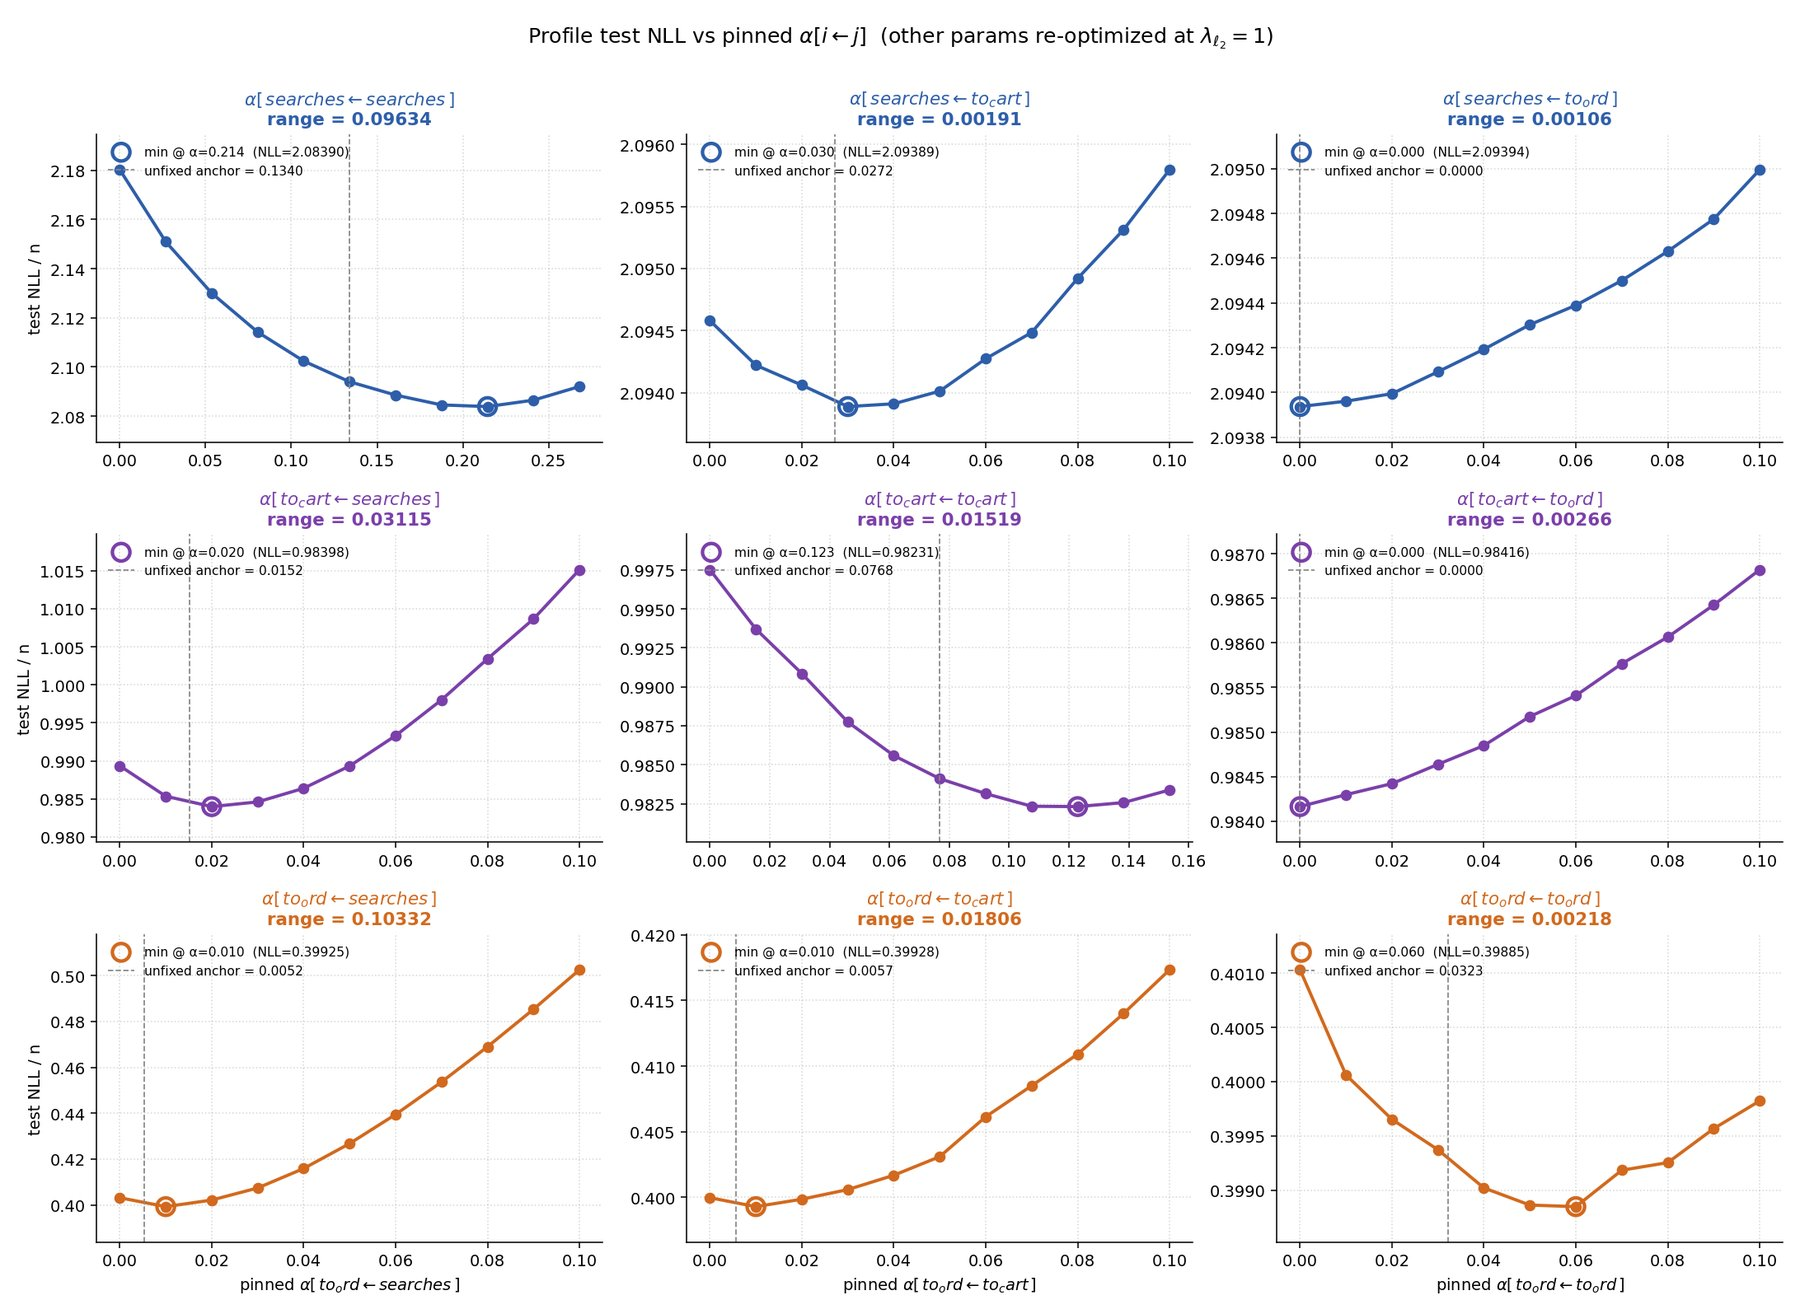
\includegraphics[width=0.85\textwidth]{images/fig25_test_nll_grid.jpg}
\caption{Test NLL profile по 9 коэффициентам}
\end{figure}


Топология profile'ей характеризуется тремя группами:

\begin{itemize}
  \item \textbf{Жёсткие коэффициенты} ($range NLL \geq  0.03$): \texttt{to\_ord ← searches} (range test NLL \texttt{0.103}), \texttt{searches ← searches} (\texttt{0.096}), \texttt{to\_cart ← searches} (\texttt{0.031}). Здесь данные \textbf{реально различают} значения коэффициента - profile NLL имеет ярко выраженный минимум.
  \item \textbf{Плоские коэффициенты} ($range NLL \leq  0.005$): вся колонка $\alpha [* \leftarrow  to\_ord]$ плюс $\alpha [searches \leftarrow  to\_cart]$ и \textbf{$\alpha [to\_ord \leftarrow  to\_ord]$} (range \texttt{0.002}). Данные на эти значения практически не реагируют - profile NLL почти константа.
  \item \textbf{Промежуточные}: \texttt{to\_ord ← to\_cart} (\texttt{0.018}), \texttt{to\_cart ← to\_cart} (\texttt{0.015}).
\end{itemize}


Топология не зависит от prior'а: control-эксперимент без регуляризации ($\lambda _{\ell_2} = 0$, $\lambda _\alpha  = 0$) даёт практически те же range'и (с расхождением во втором-третьем знаке). Это \textbf{структурный аргумент}: профили - это свойство геометрии данных, а не выбор регуляризации.

Особенно интересно, что диагональный $\alpha [to\_ord \leftarrow  to\_ord]$ оказался \textbf{плоским}, несмотря на то, что в линейном фите получает ненулевое значение \texttt{\textasciitilde{}0.03}. Это объясняется теоретически известной проблемой [4, 5]: history-state \texttt{z\textasciicircum{}\{(k)\}} диагонального канала имеет среднее

\[
\mathbb{E}[z_{u,t}^{(k)}] \;\propto\; \lambda_u^{(k)} \cdot b_t,
\]

- тот же сигнал, что и бейзлайн-часть $\lambda _u \cdot  b\_t$. Линейная комбинация двух почти коллинеарных регрессоров создаёт \textbf{ridge-подобный «жёлоб» в parameter space}: множество значений $(\lambda _u, \alpha _{kk})$ даёт почти одинаковую $\hat{\lambda}$. Для внедиагональных коэффициентов \texttt{z\textasciicircum{}\{(j)\}} относится к другому каналу, не коллинеарному бейзлайну, и коэффициент идентифицируется устойчиво.

В литературе эта же проблема обсуждается в двух подходах:

\begin{itemize}
  \item Bacry, Bompaire, Gaïffas, Muzy [4] предлагают \textbf{separate regularization} для диагональных (\texttt{ℓ\_1}-штраф) и внедиагональных (trace norm) элементов, именно потому, что диагональ absorbs baseline mass.
  \item Achab, Bacry, Gaïffas, Mastromatteo, Muzy [5] отказываются от MLE в пользу \textbf{integrated cumulants}, чтобы обойти diagonal/baseline non-identifiability на коротких выборках.
\end{itemize}


В нашей работе мы не используем эти методы напрямую - мы признаём диагональ слабо идентифицируемой и формализуем это через интервалы значений вместо точечной оценки (раздел 6.4).

Структурный смысл наблюдения: \textbf{в линейной additive Хоукс-форме с непустым бейзлайном неидентифицируемость диагонали - общее свойство, а не артефакт нашей конкретной модели}. Это согласуется с тем, что мы видим эмпирически: диагональные элементы дрейфуют под изменением регуляризации, внедиагональные - более стабильны.

Сравнение train и test profile'ей при этом неоднородно по структуре матрицы. Внедиагональные коэффициенты ведут себя стабильно: train и test profiles на них совпадают по топологии и положению минимума - данных хватает, чтобы оценка не была артефактом обучения. Диагональные же коэффициенты ведут себя иначе: на них train и test profiles \textbf{различаются заметно}, train склонен показывать более узкий и глубокий минимум, чем test, - то есть на диагонали модель легко переобучается под тренировочный сигнал. Это согласуется с тем выводом, что диагональ слабо идентифицируется на коротких выборках, а её точечная оценка зависит не столько от данных, сколько от регуляризатора.

\FloatBarrier
\subsection{Интервалы 10\%-gain и финальная матрица}

Из плоского profile NLL следует, что точечная оценка $\alpha [i, j]$ для плоских коэффициентов малоинформативна. Корректнее говорить \textbf{интервалом}: значение лежит где-то в широком диапазоне, и модель не различает точки внутри него.

Формализуем это так. Для каждой пары \texttt{(target, source)}:

\begin{itemize}
  \item \texttt{PG\_NLL(target)} - test NLL Personalized GP scaler'а (baseline без Hawkes);
  \item \texttt{min\_NLL} - минимум test NLL Joint Hawkes по 11 точкам сетки из раздела 6.3 (без регуляризации, чтобы исключить prior-эффекты);
  \item \texttt{gain = PG\_NLL - min\_NLL} - выигрыш Hawkes над baseline;
  \item \texttt{threshold = min\_NLL + 0.10 · gain}.
\end{itemize}


Допустимы такие $\alpha $, при которых модель сохраняет минимум \textbf{90\% выигрыша} над baseline. Из 11 точек профиля берётся наибольший contiguous диапазон вокруг argmin, где $test\_NLL \leq  threshold$. На границах - линейная интерполяция между соседними сеточными точками. $\alpha _lo$, $\alpha _hi$ - границы интервала, $\alpha _mid = (\alpha _lo + \alpha _hi) / 2$.


\begin{figure}[ht]
\centering
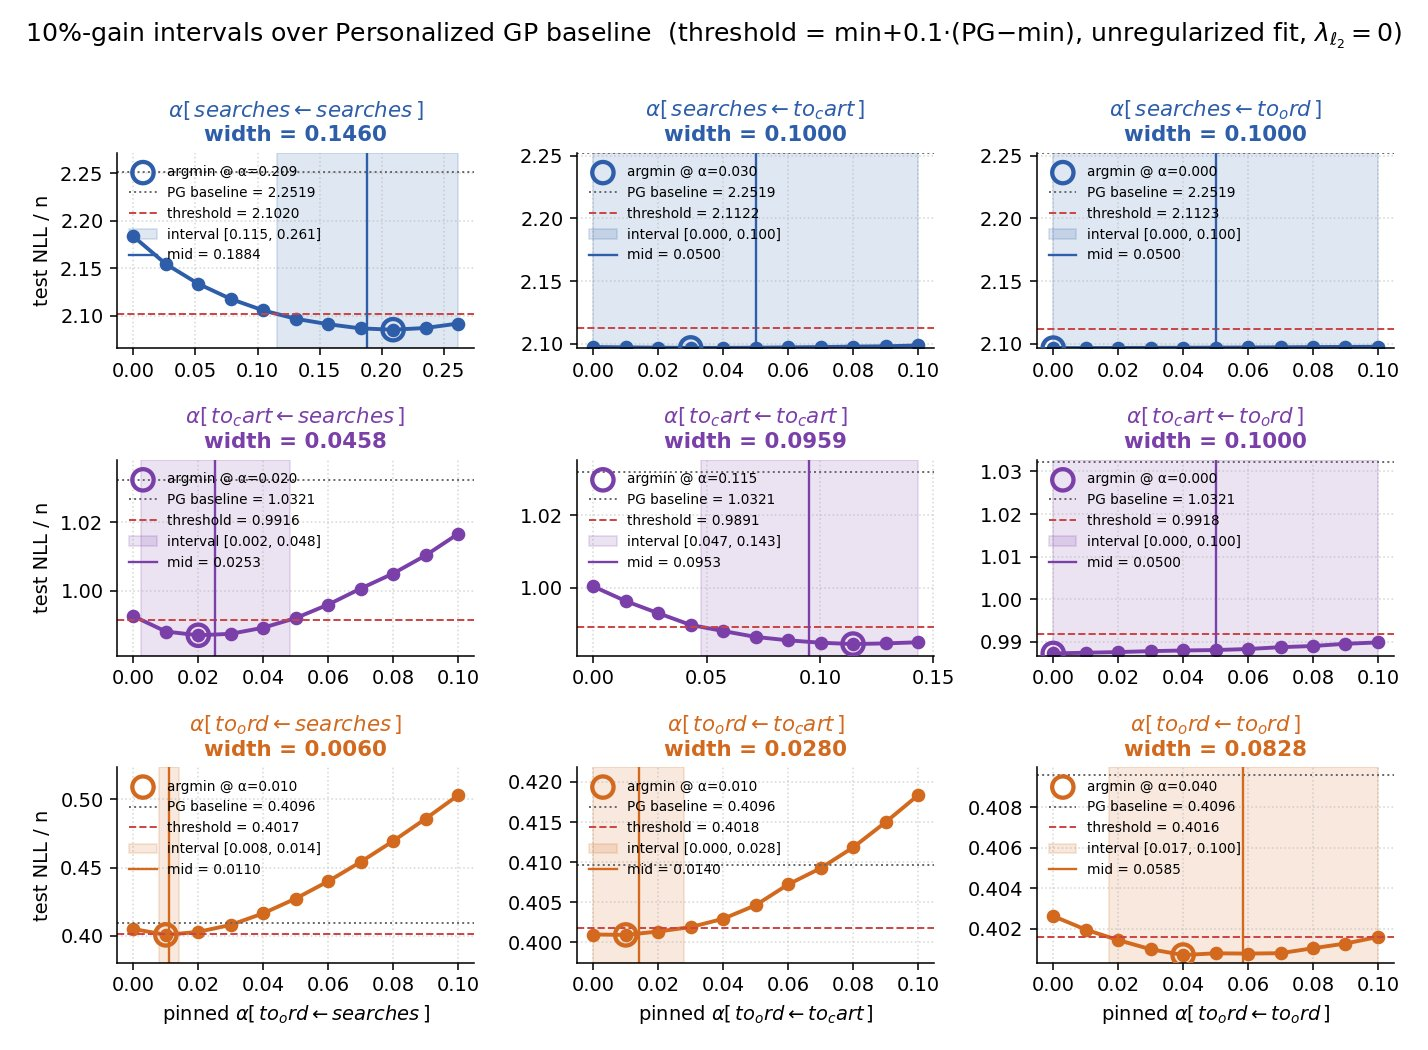
\includegraphics[width=0.85\textwidth]{images/fig26_intervals_grid.jpg}
\caption{Интервалы 10\%-gain для 9 коэффициентов}
\end{figure}


Численные результаты:


\begin{table}[ht]
\centering
\small
\begin{tabular}{lrrrr}
\toprule
target $\leftarrow$ source & $\alpha$\_lo & $\alpha$\_hi & \textbf{$\alpha$\_mid} & width \\
\midrule
\texttt{searches ← searches} & \texttt{0.115} & \texttt{0.261} & \textbf{\texttt{0.188}} & \texttt{0.146} \\
\texttt{to\_cart ← searches} & \texttt{0.002} & \texttt{0.048} & \textbf{\texttt{0.025}} & \texttt{0.046} \\
\texttt{to\_cart ← to\_cart} & \texttt{0.047} & \texttt{0.143} & \textbf{\texttt{0.095}} & \texttt{0.096} \\
\texttt{to\_ord ← searches} & \texttt{0.008} & \texttt{0.014} & \textbf{\texttt{0.011}} & \texttt{0.006} \\
\texttt{to\_ord ← to\_cart} & \texttt{0.000} & \texttt{0.028} & \textbf{\texttt{0.014}} & \texttt{0.028} \\
\texttt{to\_ord ← to\_ord} & \texttt{0.017} & \texttt{0.100} & \textbf{\texttt{0.059}} & \texttt{0.083} \\
\bottomrule
\end{tabular}
\end{table}


Три ячейки верхнего треугольника (\texttt{searches ← to\_cart}, \texttt{searches ← to\_ord}, \texttt{to\_cart ← to\_ord}) имеют плоские профили с $range \leq  0.003$ в NLL - данные на них не реагируют. \textbf{По convention воронки эти три коэффициента полагаем структурно нулевыми}: содержательно это означает, что в воронке \texttt{searches → cart → order} обратных краткосрочных эффектов нет.

Финальная матрица midpoint'ов (рис. 25):


\begin{figure}[ht]
\centering
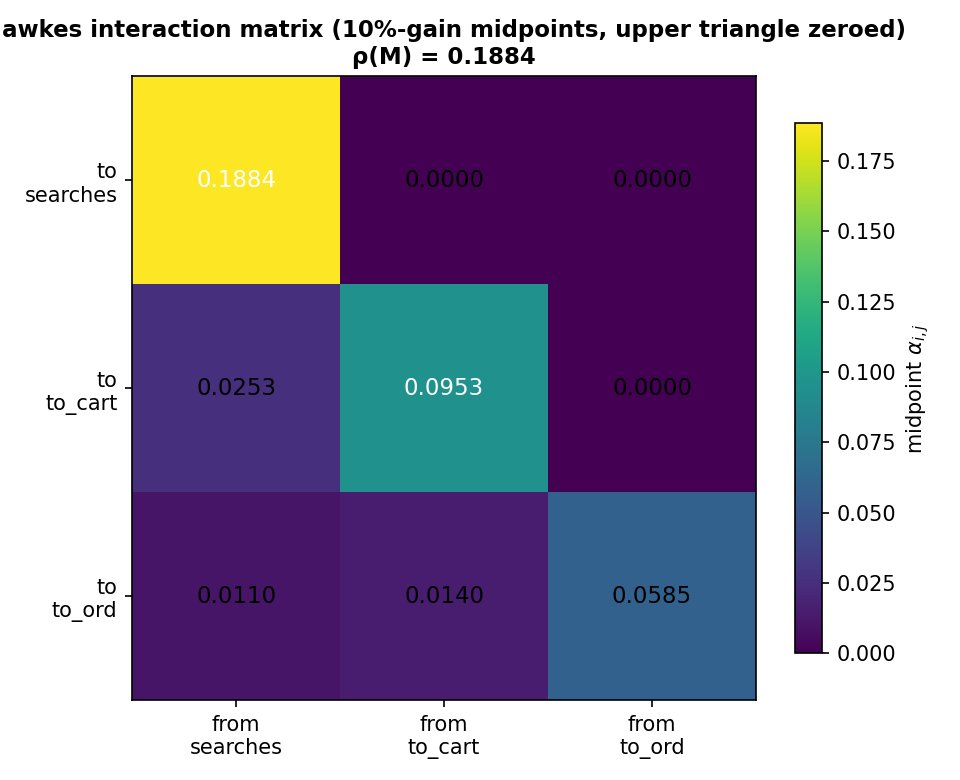
\includegraphics[width=0.85\textwidth]{images/fig27_midpoint_matrix.jpg}
\caption{Финальная Хоукс-матрица midpoint'ов}
\end{figure}



\begin{table}[ht]
\centering
\small
\begin{tabular}{lrrr}
\toprule
target ↓ \textbackslash{} source $\to$ & \texttt{searches} & \texttt{to\_cart} & \texttt{to\_ord} \\
\midrule
\texttt{searches} & \textbf{\texttt{0.188}} & \texttt{0} & \texttt{0} \\
\texttt{to\_cart} & \texttt{0.025} & \textbf{\texttt{0.095}} & \texttt{0} \\
\texttt{to\_ord} & \texttt{0.011} & \texttt{0.014} & \textbf{\texttt{0.059}} \\
\bottomrule
\end{tabular}
\end{table}


Матрица нижнетреугольная по convention funnel, поэтому собственные значения совпадают с диагональю: \texttt{|eigvals| = [0.059, 0.095, 0.188]}. Спектральный радиус $\rho (M) = 0.188$ сильно меньше единицы - Хоукс-процесс далёк от explosion-порога и описывает stable multivariate Hawkes.

Для сравнения: спектральный радиус point-mean матрицы от Scaled-baseline ch.12.4 был $\rho (\alpha _Scaled) \approx  0.082$, от Joint Hawkes c $\lambda _{\ell_2} = 1$ - $\rho  \approx  0.107$. То, что финальный midpoint-радиус \texttt{0.188} выше - естественное следствие выбора верхней границы 10\%-интервала вместо mean'а.

Это \textbf{финальный интерпретируемый результат cross-channel анализа}: 6-параметрическая нижнетреугольная матрица, описывающая стабильную self-exciting структуру воронки \texttt{searches → to\_cart → to\_ord} с явно нулевыми «обратными» рёбрами. Внутри широких 10\%-интервалов это один интерпретируемый midpoint'овый ответ - точечная оценка, к которой можно обращаться в дальнейших задачах (например, при оценке cross-channel эффектов A/B-теста).

\FloatBarrier
\subsection{Per-user визуализация работы моделей}

Чтобы понять различия Personalized GP и Joint Hawkes на уровне отдельных пользователей, мы строим для четырёх типичных юзеров timeline предсказанной интенсивности с фактическими покупками. Выборка пользователей сделана так:

\begin{itemize}
  \item \textbf{активный} (\texttt{612605}): \texttt{Y\_train = 321}, \texttt{Y\_test = 93}. Регулярная высокая активность.
  \item \textbf{малоактивный} (\texttt{238812}): \texttt{Y\_train = 6}, \texttt{Y\_test = 2}. Редкие изолированные покупки.
  \item \textbf{Joint Hawkes выигрывает} (\texttt{676128}): \texttt{Y\_train = 7}, \texttt{Y\_test = 97}, \texttt{ΔLL(JH - GP) = +151.7}. Скачок активности к концу окна.
  \item \textbf{Joint Hawkes проигрывает} (\texttt{47946}): \texttt{Y\_train = 899}, \texttt{Y\_test = 359}, \texttt{ΔLL = -134.8}. Сверхактивный пользователь с большой дневной дисперсией.
\end{itemize}


Траектории Personalized GP - рис. 26, Joint Hawkes - рис. 27.


\begin{figure}[ht]
\centering
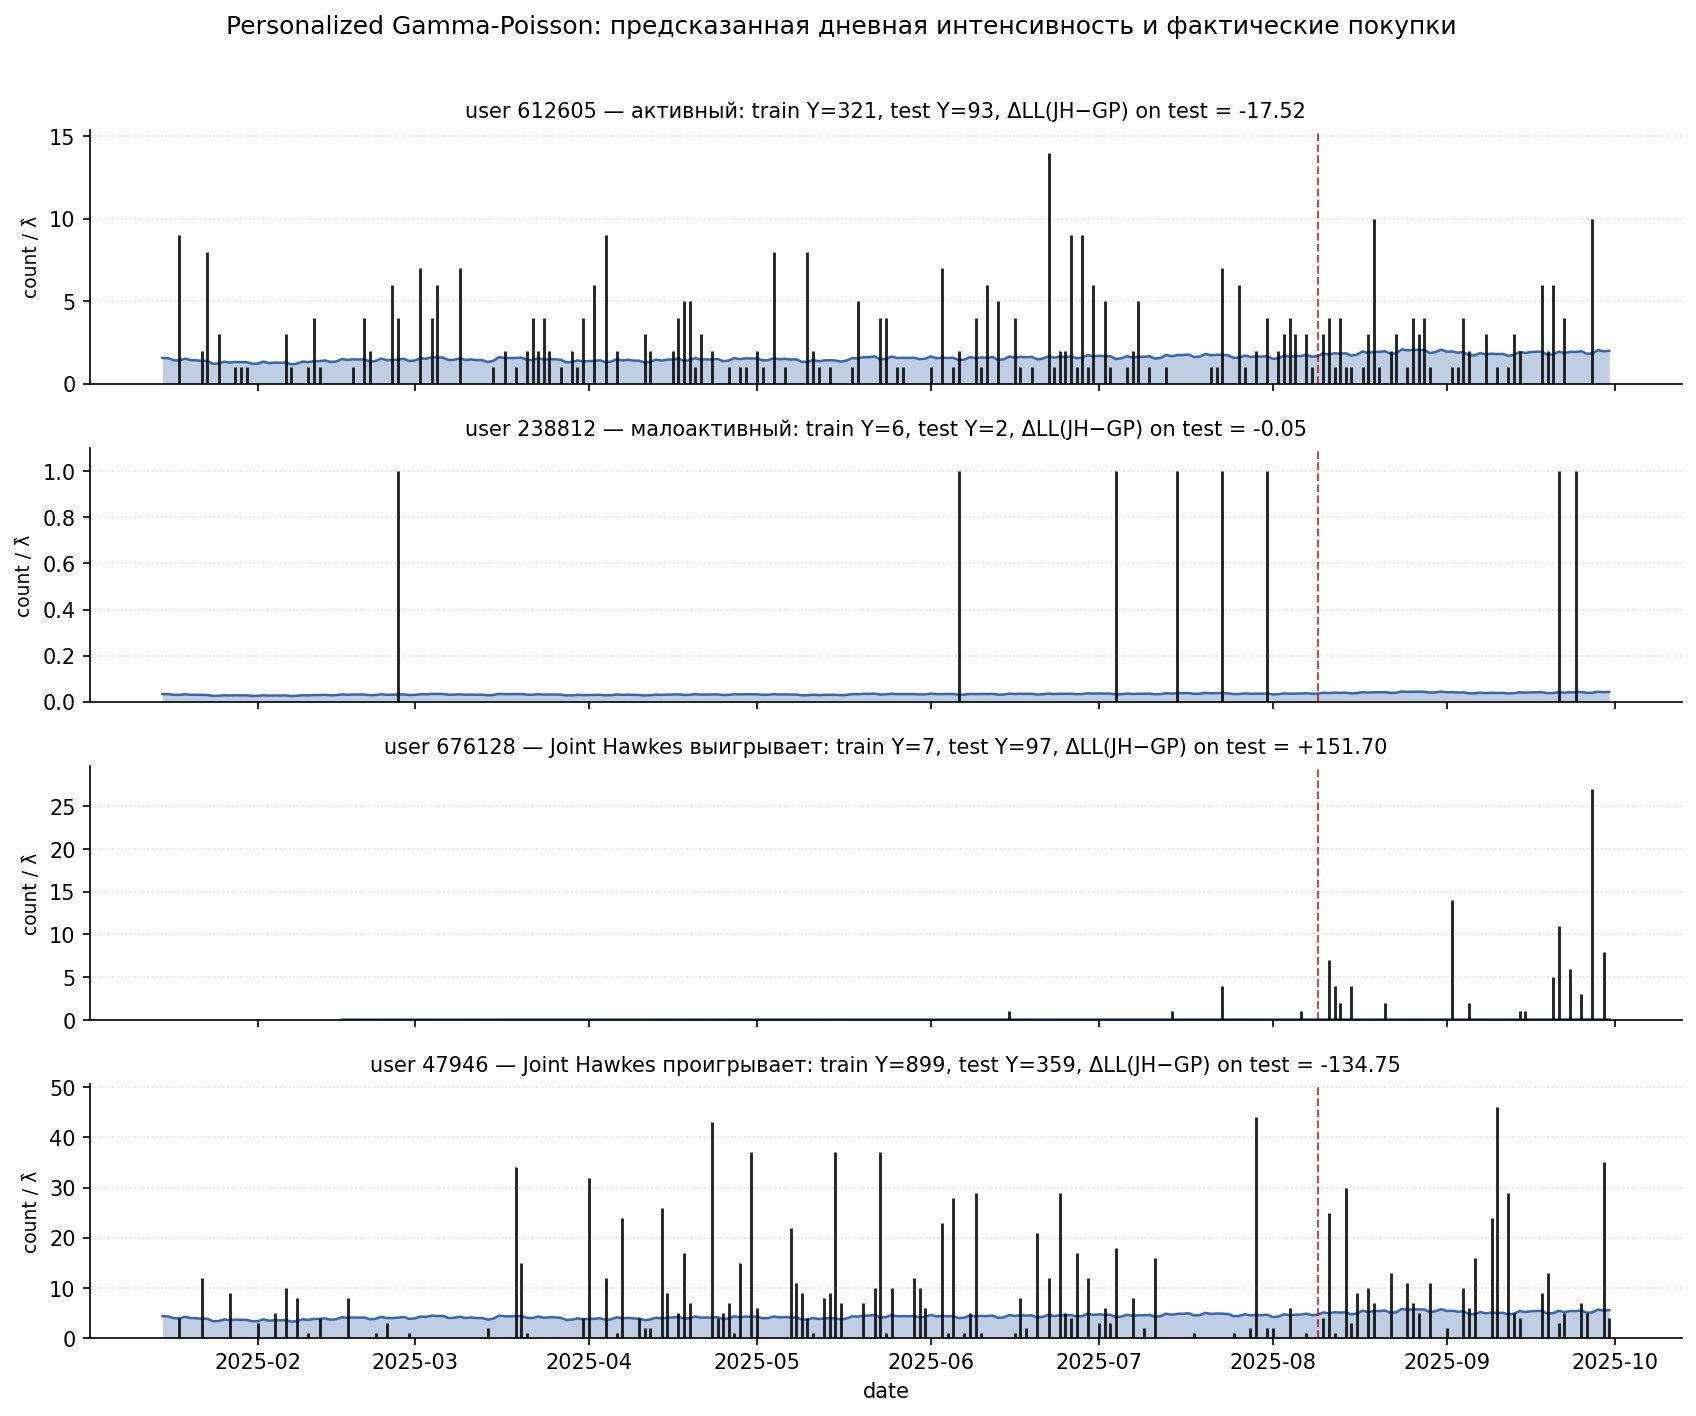
\includegraphics[width=0.85\textwidth]{images/fig28_personalized_gp_traces.jpg}
\caption{Personalized GP: traces 4 пользователей}
\end{figure}


\begin{figure}[ht]
\centering
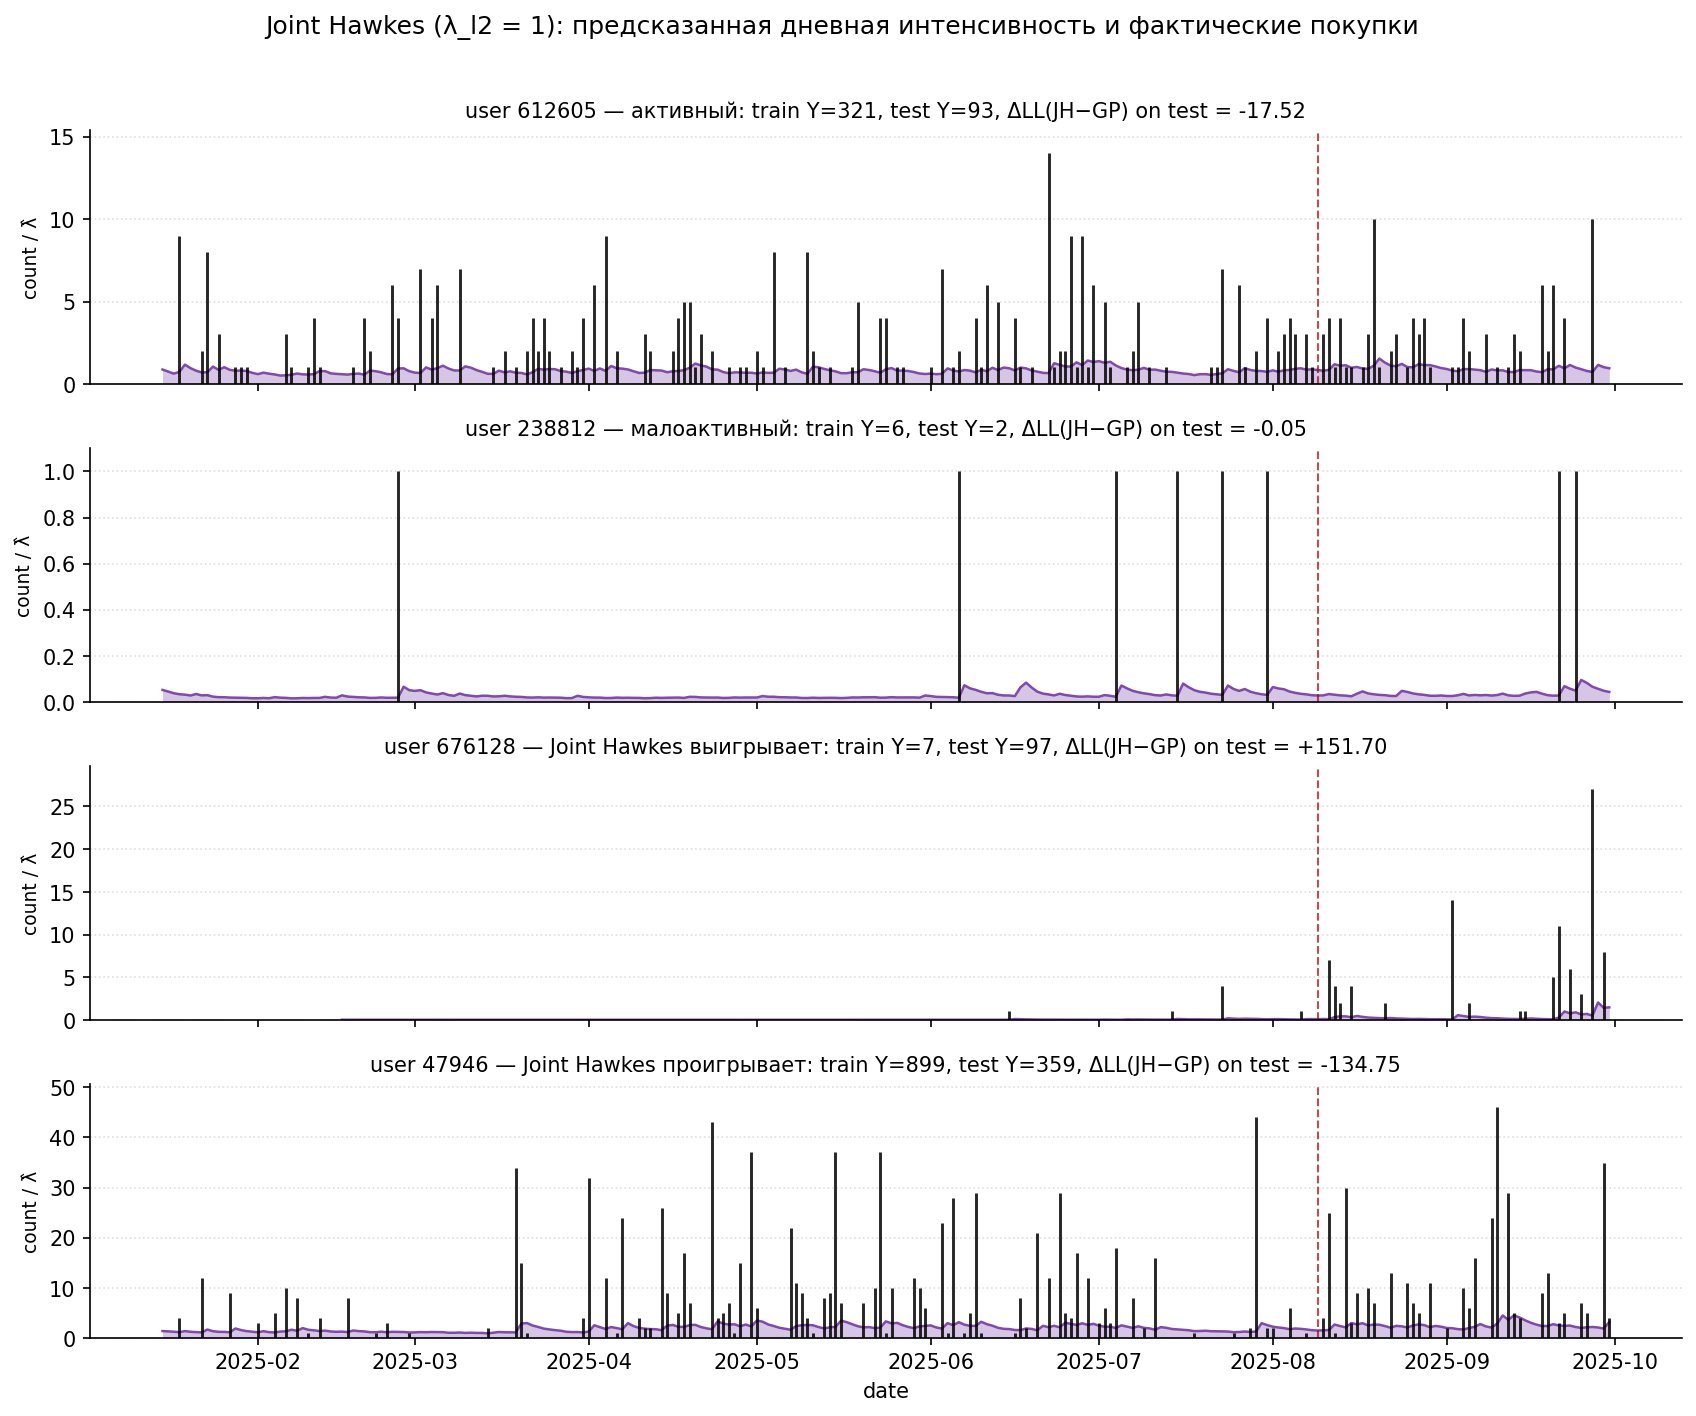
\includegraphics[width=0.85\textwidth]{images/fig29_joint_hawkes_traces.jpg}
\caption{Joint Hawkes: traces 4 пользователей}
\end{figure}


У Personalized GP интенсивность практически постоянна для каждого пользователя - модель оценивает один числовой уровень $\mu _u^{EB} \cdot  b\_t$ и его экстраполирует. Поправка от \texttt{b\_t} мала (±5\% внутри недели через Rolling Seasonal). У Joint Hawkes интенсивность \textbf{динамическая}: после каждого события $\hat{\lambda}$ экспоненциально подсвечивается и спадает к baseline с полураспадом 1-3 дня. Высота всплесков зависит от обученных $\alpha $-весов и непосредственно от текущего состояния \texttt{z\_\{u,t\}}.

Failure-modes двух моделей \textbf{дополняют друг друга}:

\begin{itemize}
  \item На малоактивном пользователе обе модели дают практически одинаковый средний уровень (\texttt{\textasciitilde{}0.04}), и разница $ΔLL \approx  −0.05$ пренебрежимо мала.
  \item На активном пользователе обе модели близки по среднему (\texttt{\textasciitilde{}1.5..2}/день), но Joint Hawkes пульсирует, иногда overshoots и теряет немного на test (\texttt{ΔLL = -17.5}).
  \item На пользователе с резким переходом режима (\texttt{676128}, мало покупок на train, всплеск на test) Joint Hawkes значительно выигрывает, потому что подхватывает начало роста через Hawkes-states: интенсивность поднимается до \texttt{5..10} в дни streak'ов. Pers GP остаётся flat у \texttt{\textasciitilde{}0.1} и платит большой NLL за каждый ненулевой день. \texttt{ΔLL = +151.7}.
  \item На сверхактивном пользователе с высокой дневной дисперсией (\texttt{47946}) Joint Hawkes overreacts на крупные одиночные дни (где \texttt{y = 30..45}), и его $\hat{\lambda}$ доходит до \texttt{20+}, тогда как на следующий день у пользователя часто только \texttt{2..3} покупки. Pers GP с более консервативным средним уровнем (\texttt{\textasciitilde{}4..5}) лучше согласуется. \texttt{ΔLL = -134.8}.
\end{itemize}


На уровне population-NLL разница между моделями скромная (\texttt{0.3958} vs \texttt{0.3951}), но per-user \texttt{ΔLL} распределена сильно неоднородно - \texttt{±150} для отдельных пользователей при mean'е $\approx  0$. Это означает, что \textbf{с точки зрения общего качества модели почти эквивалентны, но в индивидуальных предсказаниях они существенно различны}. Для бизнес-применения (например, ранжирование пользователей по ожидаемой выручке) это может быть важно: одна и та же population-метрика может скрывать разные паттерны ошибок.

\clearpage
\section{Заключение}

В работе исследовано применение процессов Хокса для предсказания дневной интенсивности покупок пользователя в e-commerce-сервисе на датасете из \texttt{\textasciitilde{}10K} пользователей за \texttt{\textasciitilde{}290} дней. Основные результаты сгруппированы по трём ветвям исследования.

\textbf{Бейзлайн и Хоукс-надстройка на полном train-test (часть I).} Построена последовательность из шести вероятностных моделей с переходом от Global Poisson к Joint Hawkes. Самый крупный единичный шаг по test NLL - переход к Personalized Gamma-Poisson через Empirical Bayes (\texttt{+24K} в LL / \texttt{-0.048} в NLL). Хоукс-надстройка над персонализированным бейзлайном даёт стабильное улучшение порядка \texttt{+7K} в LL / \texttt{-0.014} в NLL на каждом из трёх независимых каналов воронки (\texttt{searches}, \texttt{to\_cart}, \texttt{to\_ord}). Контрольный GBDT на полном feature-engineering'е (141 фича) обходит Hawkes ещё на \texttt{2..3\%} от бейзлайна NLL, занимая верхнюю планку по качеству. При этом Hawkes закрывает \texttt{54..77\%} общего gap'а от Pers GP до GBDT при существенно меньшем числе параметров и сохранённой интерпретируемости. Анализ per-user delta-LL показывает, что Хоукс-надстройка работает равномерно по всем бакетам активности, в отличие от персонализации, которая даёт перекосы на средне-активных пользователях.

\textbf{Поведение на коротких train-окнах (часть II).} На коротких train (\texttt{14..50} дней) Scaled-baseline Hawkes \textbf{вырождается} в Personalized GP: оптимизатор не находит дополнительного сигнала для Хоукс-надстройки из-за коллинеарности EB-shrunk базы и редких target-событий. Joint Hawkes с активной L2-регуляризацией $(\lambda _u - 1)^2$ решает эту проблему: при том же предсказательном качестве на длинных train он не вырождается на коротких. Train-length scan по $n \in  [15, 200]$ дней демонстрирует чёткий crossover: на $n \leq  21$ лидирует Joint Hawkes, на $n \in  [27, 60]$ все модели сходятся, на $n \geq  100$ оба Хоукс-варианта эквивалентны и оба обходят Personalized GP. Для индустриальной практики это означает, что в системе с переменной длиной окна Joint Hawkes является более безопасным default-выбором.

\textbf{Структура cross-channel Хоукс-матрицы (часть III).} Cross-channel матрица $\alpha  \in  \mathbb{R}^{3\times 3}$ имеет интерпретируемую структуру: верхнетреугольные коэффициенты ($\alpha [searches \leftarrow  to\_cart]$, $\alpha [searches \leftarrow  to\_ord]$, $\alpha [to\_cart \leftarrow  to\_ord]$) идентически нулевые - отражают отсутствие краткосрочного «обратного» возбуждения в воронке. Off-diagonal funnel-связи \texttt{searches → cart → order} положительны и идентифицируемы стабильно ($CV \leq  16\%$ в bootstrap по 10$\times$100d-окнам). Диагональные коэффициенты - особенно $\alpha [to\_ord \leftarrow  to\_ord]$ - обладают принципиальной слабой идентифицируемостью: profile NLL почти плоский на широком диапазоне значений. Это структурное следствие коллинеарности history-state и baseline и согласуется с известными в литературе результатами по multivariate Hawkes [4, 5]. Sweep по силе L2-prior'а $\lambda _{\ell_2} \in  [0, 5]$ показывает, что регуляризация существенно перераспределяет массу между бейзлайн-частью $\lambda _u \cdot  b\_t$ и Хоукс-надстройкой $\alpha ^{\top} z$ (особенно на редком \texttt{to\_ord}), но \textbf{почти не влияет на predicted intensity на test} (range NLL $\leq$ \texttt{0.01}). На уровне внутренних параметров модель сверх-параметризована: множество разных $(\lambda _u, \alpha )$-решений даёт почти одинаковый скор. После формализации через 10\%-gain интервалы получена финальная нижнетреугольная матрица midpoint'ов со спектральным радиусом $\rho (M) = 0.188$, описывающая стабильный multivariate Хоукс-процесс.

\textbf{Практические выводы}. Хоукс-модель в виде Joint Hawkes с активной L2-регуляризацией пригодна для прогноза покупок в задачах с коротким и длинным train; она даёт хороший trade-off между предсказательным качеством и интерпретируемостью; cross-channel матрица $\alpha $ допускает прямую интерпретацию как структуру self-excitation воронки и может использоваться для анализа эффектов на конкретные каналы (например, при подведении итогов A/B-эксперимента с дополнительной декомпозицией эффекта). Tree-ensemble остаётся лучшим в абсолюте, но без структуры - выбор между Hawkes и GBDT определяется приоритетом интерпретируемости над skoring'ом. Per-user визуализация показывает, что даже при близких population-метриках Hawkes и Personalized GP дают существенно разные индивидуальные предсказания, и это нужно учитывать при downstream-применении модели.

\textbf{Направления дальнейшей работы}: расширение feature-set для Hawkes-states (включение более длинных полураспадов, категориальных контекстов или session-level фичей); исследование adaptive-регуляризации диагональных коэффициентов в духе раздельной L1/trace norm [4], или замена MLE на integrated cumulants [5]; применение модели к A/B-тестированию с явным cross-channel разложением эффекта; интеграция Хоукс-надстройки с нейросетевым кодером истории в духе RMTPP [3] или Neural Hawkes [7], как способ объединить интерпретируемость $\alpha$-матрицы с гибкостью deep representation'ов.


\begin{thebibliography}{99}

\bibitem{ref-1} Hawkes A. G. \textbf{Spectra of some self-exciting and mutually exciting point processes} // Biometrika. - 1971. - Vol. 58, No. 1. - P. 83-90.
\bibitem{ref-2} Bacry E., Mastromatteo I., Muzy J.-F. \textbf{Hawkes processes in finance} // Market Microstructure and Liquidity. - 2015. - Vol. 1, No. 1. - 1550005.
\bibitem{ref-3} Du N., Dai H., Trivedi R., Upadhyay U., Gomez-Rodriguez M., Song L. \textbf{Recurrent marked temporal point processes: Embedding event history to vector} // Proceedings of KDD. - 2016. - P. 1555-1564.
\bibitem{ref-4} Bacry E., Bompaire M., Gaïffas S., Muzy J.-F. \textbf{Sparse and low-rank multivariate Hawkes processes} // Journal of Machine Learning Research. - 2020. - Vol. 21, No. 50. - P. 1-32.
\bibitem{ref-5} Achab M., Bacry E., Gaïffas S., Mastromatteo I., Muzy J.-F. \textbf{Uncovering causality from multivariate Hawkes integrated cumulants} // Journal of Machine Learning Research. - 2018. - Vol. 18, No. 192. - P. 1-28.
\bibitem{ref-6} Fader P. S., Hardie B. G. S., Lee K. L. \textbf{RFM and CLV: Using iso-value curves for customer base analysis} // Journal of Marketing Research. - 2005. - Vol. 42, No. 4. - P. 415-430.
\bibitem{ref-7} Mei H., Eisner J. \textbf{The neural Hawkes process: A neurally self-modulating multivariate point process} // Advances in Neural Information Processing Systems. - 2017. - Vol. 30. - P. 6754-6764.
\bibitem{ref-8} Friedman J. H. \textbf{Greedy function approximation: A gradient boosting machine} // The Annals of Statistics. - 2001. - Vol. 29, No. 5. - P. 1189-1232.

\end{thebibliography}
\end{document}
